%%%%%%%%%%%%%%%%%%%%%%%%%%%%%%%%%%%%%%%%%%%%%%%%%%%%%%%%%%%%%%%%%%%%%%%%%%%%%%%%
%2345678901234567890123456789012345678901234567890123456789012345678901234567890
%        1         2         3         4         5         6         7         8

\documentclass[letterpaper, 10 pt, conference]{ieeeconf}  % Comment this line out if you need a4paper

%\documentclass[a4paper, 10pt, conference]{ieeeconf}      % Use this line for a4 paper

\IEEEoverridecommandlockouts                              % This command is only needed if 
                                                          % you want to use the \thanks command

\overrideIEEEmargins                                      % Needed to meet printer requirements.

%In case you encounter the following error:
%Error 1010 The PDF file may be corrupt (unable to open PDF file) OR
%Error 1000 An error occurred while parsing a contents stream. Unable to analyze the PDF file.
%This is a known problem with pdfLaTeX conversion filter. The file cannot be opened with acrobat reader
%Please use one of the alternatives below to circumvent this error by uncommenting one or the other
%\pdfobjcompresslevel=0
%\pdfminorversion=4

% See the \addtolength command later in the file to balance the column lengths
% on the last page of the document

% The following packages can be found on http:\\www.ctan.org
\usepackage{graphics} % for pdf, bitmapped graphics files
\usepackage{epsfig} % for postscript graphics files
% \usepackage{mathptmx} % assumes new font selection scheme installed
\usepackage{times} % assumes new font selection scheme installed
\usepackage{amsmath} % assumes amsmath package installed
\usepackage{amssymb}  % assumes amsmath package installed
\usepackage[ruled,vlined,linesnumbered]{algorithm2e}
\SetAlgoSkip{}
\usepackage{hyperref}
\usepackage{bm}
\usepackage{gensymb}
\usepackage{caption}
\captionsetup[table]{position=bottom}   %% or below
\usepackage{subcaption}
\usepackage{xcolor}
\usepackage{svg}
\usepackage{wrapfig}
% \usepackage{algorithm,algorithmicx,algpseudocode}
\usepackage{algpseudocode}
\usepackage{booktabs}
\usepackage{threeparttable}
\usepackage{array} % <-- new
\newcolumntype{C}[1]{>{\centering\arraybackslash}p{#1}} % <-- ne
\newtheorem{theorem}{Theorem}
\newtheorem{corollary}{Corollary}[theorem]
\newtheorem{lemma}[theorem]{Lemma}
\newtheorem{definition}{Definition}
\newtheorem{problem}{Problem}
\DeclareMathOperator{\interior}{int}
\DeclareMathOperator{\diag}{diag}

%\setlength{\textfloatsep}{5pt}
%\renewcommand{\baselinestretch}{1}

\newcommand{\R}{\mathbb{R}}
\newcommand{\Ncal}{\mathcal{N}}
\newcommand{\by}{\mathbf{y}}
\newcommand{\bx}{\mathbf{x}}
\newcommand{\bz}{\mathbf{z}}
\newcommand{\bW}{\mathbf{W}}
\newcommand{\bb}{\mathbf{b}}
\newcommand{\btheta}{\mathbf{\theta}}
\newcommand{\bTheta}{\mathbf{\Theta}}
\newcommand{\blambda}{\mathbf{\lambda}}
\newcommand{\bLambda}{\mathbf{\Lambda}}
\newcommand{\ba}{\mathbf{a}}
\newcommand{\bA}{\mathbf{A}}
\newcommand{\bC}{\mathbf{C}}
\newcommand{\bd}{\mathbf{d}}
\newcommand{\bdelta}{\mathbf{\delta}}
\newcommand\scalemath[2]{\scalebox{#1}{\mbox{\ensuremath{\displaystyle #2}}}}

\newenvironment{rcases}
  {\left.\begin{aligned}}
  {\end{aligned}\right\rbrace}

\title{\LARGE \bf
Reachable Polyhedral Marching (RPM): An Exact Analysis Tool for Deep-Learned Control Systems}

\author{Joseph A. Vincent$^{1}$ and Mac Schwager$^{1}$% <-this % stops a space
\thanks{$^{1}$Department of Aeronautics and Astronautics, Stanford University, Stanford, CA 94305, USA, {\texttt\small \{josephav, schwager\}@stanford.edu}}
\thanks{The first author was supported in part by a Dwight D. Eisenhower Transportation Fellowship. This work was sported in part by ONR grant N00014-23-1-2354. The NASA University Leadership Initiative (grant \#80NSSC20M0163) provided funds to assist the authors with their research, but this article solely reflects the opinions and conclusions of its authors and not any NASA entity. We are grateful for this support.}%
\thanks{Code: \href{https://github.com/StanfordMSL/Neural-Network-Reach}{\text{https://github.com/StanfordMSL/Neural-Network-Reach}}.}
}

\begin{document}

\maketitle
\thispagestyle{plain}
% \pagestyle{empty}
\pagestyle{plain}

%%%%%%%%%%%%%%%%%%%%%%%%%%%%%%%%%%%%%%%%%%%%%%%%%%
%%%%%%%%%%%%%%%%%%%%%%%%%%%%%%%%%%%%%%%%%%%%%%%%%%
\begin{abstract} \label{Abstract}
Neural networks are increasingly used in robotics as policies, state transition models, state estimation models, or all of the above.
With these components being learned from data, it is important to be able to analyze what behaviors were learned and how this affects closed-loop performance.
In this paper we take steps toward this goal by developing methods for computing control invariant sets and regions of attraction (ROAs) of dynamical systems represented as neural networks.
We focus our attention on feedforward neural networks with the rectified linear unit (ReLU) activation, which are known to implement continuous piecewise-affine (PWA) functions.
We describe the Reachable Polyhedral Marching (RPM) algorithm for enumerating the affine pieces of a neural network through an incremental connected walk.
We then use this algorithm to compute exact forward and backward reachable sets, from which we provide methods for computing control invariant sets and ROAs.
Our approach is unique in that we find these sets incrementally, without Lyapunov-based tools.
In our examples we demonstrate the ability of our approach to find non-convex control invariant sets and ROAs on tasks with learned van der Pol oscillator and pendulum models.
Further, we provide an accelerated algorithm for computing ROAs that leverages the incremental and connected enumeration of affine regions that RPM provides.
We show this acceleration to lead to a 15x speedup in our examples.
Finally, we apply our methods to find a set of states that are stabilized by an image-based controller for an aircraft runway control problem.
\end{abstract}

%%%%%%%%%%%%%%%%%%%%%%%%%
\section{Introduction}
%%%%%%%%%%%%%%%%%%%%%%%%%
\label{Sec:Introduction}
\subsection{Overview}

In this paper we describe the Reachable Polyhedral Marching (RPM) algorithm for enumerating the affine regions of neural networks with rectified linear unit (ReLU) activation.
This algorithm can then be leveraged to compute forward and backward reachable sets of neural networks.
Our algorithm provides a building block for proving safety properties for autonomous systems with learned perception, dynamics, or control components in the loop.  
Specifically, given a set in the input space, RPM computes the set of all corresponding outputs. 
Similarly, given a set of outputs, RPM computes the set of all corresponding inputs under the ReLU network.  
We use these capabilities to compute control invariant sets and regions of attraction (ROAs) for dynamical systems represented as neural networks.
Computing these sets helps roboticists (i) verify whether safety specifications on the robot state are met, (ii) identify states that will converge to some desirable equilibria, and (iii) identify regions in the state space for which a system can be controlled.
Identification of these sets is an important part of the control design process, as directly synthesizing control policies that meet invariance constraints by construction is challenging \cite{blanchini2008set}.
If a constraint is not met, the reachable or invariant sets computed give insight into which states lead to violation of the constraints, informing targeted policy improvements.

% Forward and backward reachable sets are often used in robotics to assess safety. 
% When a robot has a goal set of states to reach and an unsafe set of states to avoid, finding a forward reachable set can determine whether a set of initial states will reach the goal set and avoid the unsafe set. 
% Conversely, finding backward reachable sets of the goal and unsafe sets can determine which initial states will reach the goal and which will lead to the unsafe set. 

% While forward and backward reachable sets are useful to assess safety, the cost of computing these sets scales poorly with the number of time steps into the future or past. 
% For longer time horizons it is often more feasible to search for \textit{invariant sets}. 
% An invariant set is a set of states such that all trajectories starting within the set never leave the set.
% When all trajectories in an invariant set asymptotically converge to an equilibrium, the set is called an invariant \textit{region of attraction} (ROA).



\begin{figure}[!t]
    % \setlength\abovecaptionskip{-0.2\baselineskip}
  % \setlength\belowcaptionskip{-1.5\baselineskip}
  \centering
%   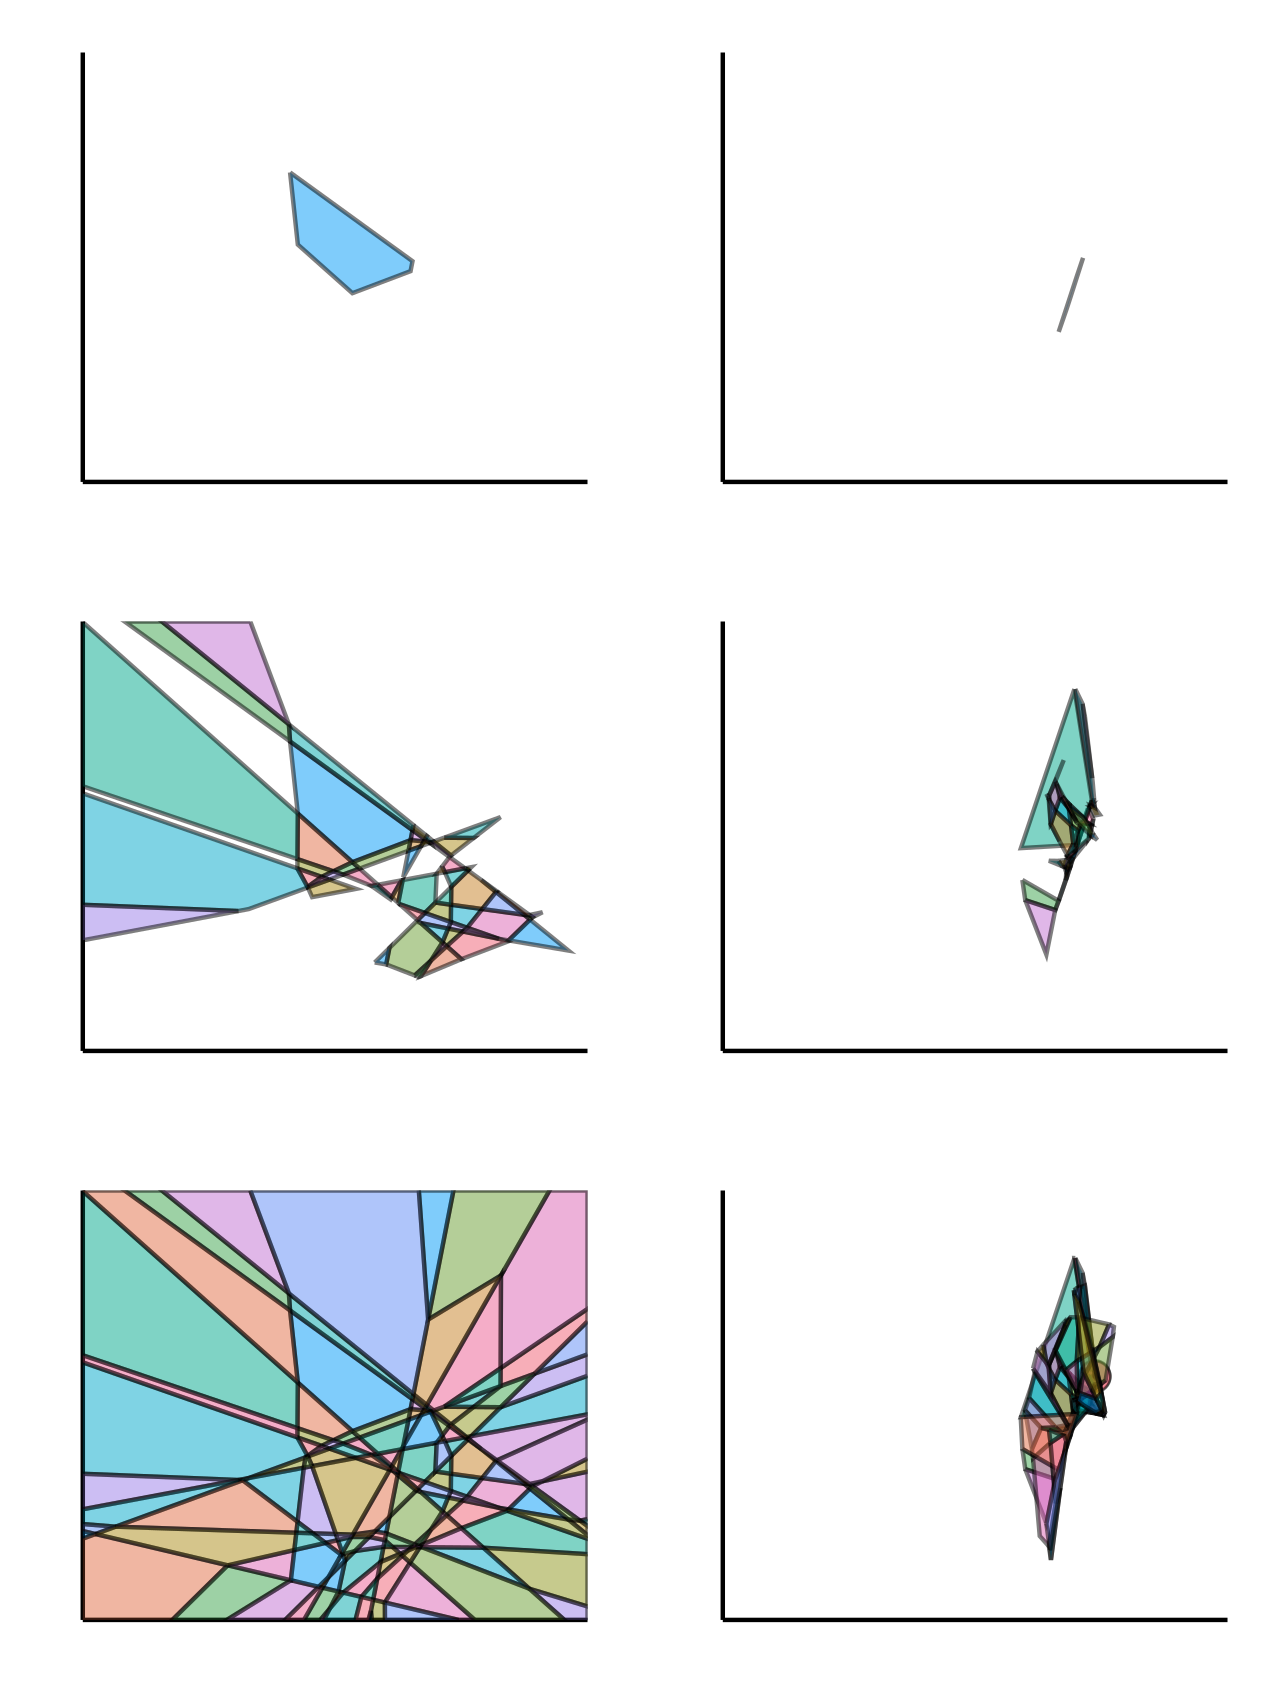
\includegraphics[width=\columnwidth]{figs/figure_1.png}
  % \includesvg[width=\columnwidth]{figs/figure_1.svg}
  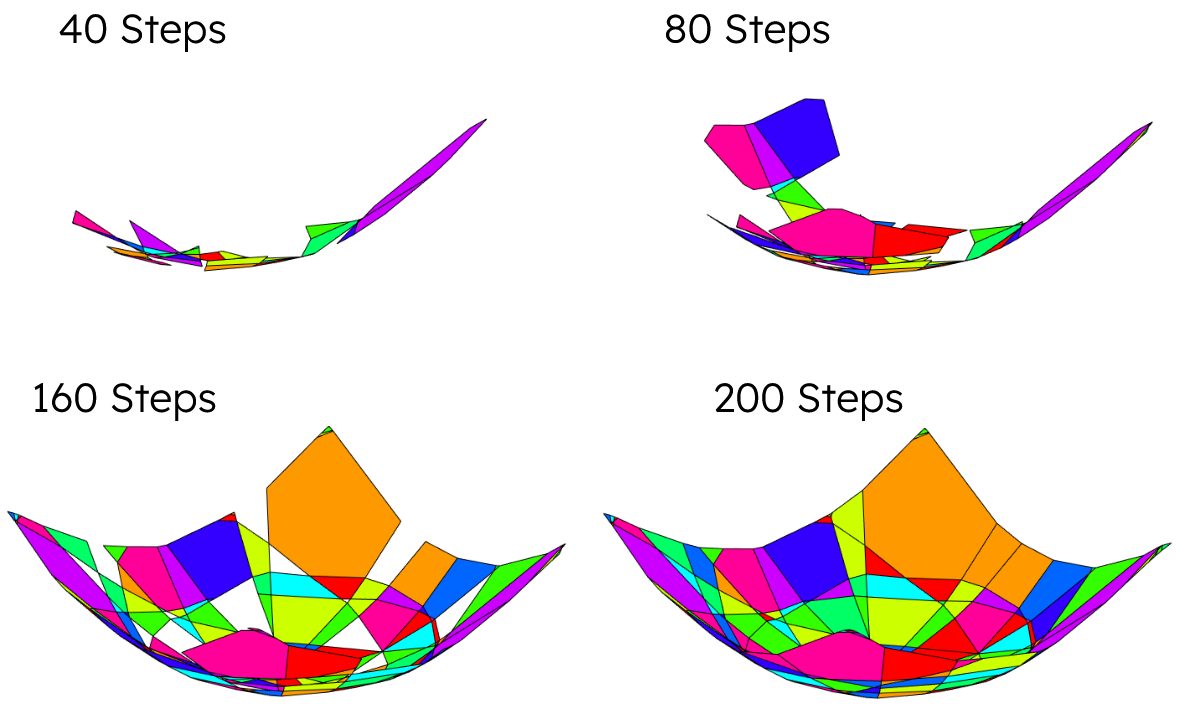
\includegraphics[width=0.85\columnwidth]{figs/figure_1_nobox.png}
  \caption{RPM's incremental enumeration of each affine region in a ReLU network. In this case the ReLU network was trained to approximate a quadratic function. Each new affine region enumerated is connected to a previous region.}
  \label{fig:cell_enum}
\end{figure}

It is well known that ReLU networks implement continuous piecewise-affine (PWA) functions, that is, the input space for a ReLU network can be tessellated into polyhedra, and over each polyhedron the neural network is affine. 
The RPM algorithm explicitly finds this equivalent PWA representation for a given ReLU network. 
Figure \ref{fig:cell_enum} illustrates how RPM incrementally solves for this representation. 
The algorithm incrementally enumerates the polyhedra and affine pieces of the PWA function by solving a series of Linear Programs (LPs), and following analytical edge flipping rules to determine neighboring polyhedra. 
The algorithm starts with an initial polyhedron, then solves for its neighboring polyhedra, then neighbors of neighbors, etc., until the desired input set is tessellated. 
In this way, our method is geometrically similar to fast marching methods in optimal control \cite{HJBFastMarching}, path planning \cite{PlanningFastMarching,FMT}, and graphics \cite{FastMarchingCubes,lei2020analytic}. 

We then use methods for PWA reachability to compute forward and backward reachable sets for each polyhedron and associated affine function. 
Computing forward and backward reachable sets allows us to search for and construct control invariant sets and ROAs without Lyapunov tools.
Finally, we also propose an accelerated backward reachability procedure that leverages the connected enumeration of the RPM algorithm to restrict the number of polyhedra the algorithm searches over.
We show that this accelerated procedure is guaranteed to enumerate the entire backward reachable set in the case that the deep network is a homeomorphism (a continuous bijection with continuous inverse).  
Checking this condition is simple, and represents a novel general procedure for examining the invertibility of neural networks whose hidden layers are not invertible themselves.

% While deep learning holds immense promise for expanding the capabilities, flexibility, and adaptability of robotic systems, currently there exists no practical method for verifying dynamic safety properties (such as stability, persistent feasibility, or forward invariance) of robotic systems with learned components.  Developing such safety verification tools is crucial if robots with learned components are to be used in safety critical applications, such as autonomous cars, aircraft, manufacturing, or search and rescue.

\subsection{Existing Work}
Most existing algorithms that compute exact reachable sets of neural networks iterate through the network layer-by-layer \cite{xiang2017reachable,nnv,yang2020reachability}. 
The layer-by-layer approaches obtain the entire reachable set at once at the end of the computation, rather than revealing the reachable set piece by piece throughout the computation. 
Consequently, if the computation must end early due to memory constraints or a computer fault, no usable result is obtained. 
In contrast, RPM builds the reachable set one polyhedron at a time, leading to a partial, but still potentially useful result if computation is halted before the algorithm runs to completion. 
% Incremental computation is better suited to finding counterexamples to safety properties and terminating early, as well as providing a more memory efficient approach where a region of the reachable set already computed can be saved externally to free up memory for remaining computation. 

\textcolor{black}{The authors of \cite{nnenum} also propose an incremental approach to visiting each affine region in a ReLU network.}
The difference between this tool and our RPM algorithm is that RPM enumerates affine regions of the neural network in a connected walk; each new region that is revealed is connected to a previous region. 
In contrast, the algorithm used in \cite{nnenum} does not have this property; whether a new region is connected to a previous one is unknown by the algorithm.
In Section \ref{Sec:ROA} we show how the connected enumeration property leads to an accelerated algorithm for computing ROAs.
Another way to conceptualize this difference between RPM and \cite{nnenum} is that RPM can also return the graph that describes which affine regions neighbor one another. \textcolor{black}{This feature is enabled by RPM's unique property of removing redundant constraints in the input-space polyhedra, resulting in the minimal description of each affine region.}

% The set of polyhedra and associated affine maps produced by our algorithm is an explicit piecewise-affine (PWA) representation of the ReLU network.  Aside from computing reachable sets, this explicit PWA representation provides useful insights such as the number of affine regions and the rank of each affine map.  Dynamical systems with PWA dynamics, known as hybrid systems, are well studied. Hence, using our method to translate a ReLU network to a PWA function, control design and analysis tools from the hybrid systems literature  \cite{invariant} can be immediately applied to dynamics with ReLU components. 

% A key challenge in verifying the safety of robots with learned components is that robots are dynamical systems, iterating their behavior over time in a feedback loop.  Existing neural network verification methods are inadequate, as they are typically not designed for iterative executions of the network in a feedback loop, are often limited to impractically small networks, and rarely consider backward reachability.  In contrast, our algorithm is designed to quickly determine reachable sets over multiple time steps into the future or the past.  Our algorithm could be used within a planning algorithm to determine, e.g., if a collision is imminent, or to perform offline verification to determine if unsafe states are reachable during execution.

 %Neural networks are increasingly used in both the modeling and control of dynamical systems. Neural networks have shown incredible potential for their usefulness in robotics, however, the realization of this potential to real-world and potentially safety-critical systems is dependent on a user's ability to verify the effectiveness and safety of these learned components. In recent years the field of neural network verification has emerged to address the problem of analyzing properties of neural networks over continuous input sets. For example, such properties may include desired input-output behavior of a learned controller, or whether a region of the state space is reachable for a learned dynamical system given a range of initial conditions.  Approaches to neural network verification can largely be characterized as reachability, optimization, and search approaches \cite{liu2019algorithms}. Reachability approaches are especially useful for analysis of learned dynamical systems. In this paper, we consider the problem of determining exact forward and backward reachable sets of a neural network given specified input and output sets, respectively. To this end we propose a novel reachability approach for the analysis of neural networks. 
 \subsection{Contributions and Organization}
\textcolor{black}{In \cite{VincentSchwagerICRA21RPM}, the RPM algorithm was introduced and demonstrated on multi-step reachability tasks. 
In contrast, the contributions of this paper are
\begin{itemize}
     \item \textcolor{black}{A formal proof of correctness for the RPM algorithm via} a theorem to analytically determine an \textcolor{black}{affine region} from its neighbor by flipping neuron activations in ReLU networks. 
     \item Application of PWA analysis tools to compute control invariant sets and regions of attraction for dynamical systems represented as ReLU networks.
     \item An accelerated exact backward reachability algorithm for ReLU networks \textcolor{black}{that does not require enumerating all affine regions}, leveraging a novel \textcolor{black}{approach} for checking the invertibility of the network.
\end{itemize}}


\textcolor{black}{Through these contributions,} we are able to compute intricate invariant sets that may be non-convex and even disconnected.
In numerical examples, we compute ROAs for a learned van der Pol oscillator, and show this computation enjoys a $15$x speedup because the learned dynamics are homeomorphic. 
We then pair RPM with the MPT3 \cite{MPT3} Matlab toolbox to find an a control invariant set for a learned torque-controlled pendulum. 
Finally, we apply our algorithm to find a set of states stabilized by an image-based airplane runway taxiing system, TaxiNet \cite{verify_gan}. 
The closed-loop system is PWA with ${\sim}250,000$ regions, orders of magnitude larger than PWA systems for which other nonlinear stability analysis approaches have been demonstrated.

The paper is organized as follows.
We give related work in Section \ref{Sec:RelatedWork} and give background and state the problem in Section \ref{Sec:Background}. 
Section \ref{Sec:PWA} describes the RPM algorithm and explains its derivation. 
In Section \ref{Sec:Reachability} we describe how RPM is used to perform forward and backward reachability computations for ReLU networks over multiple time steps. 
In Section \ref{Sec:ROA} we describe how RPM is leveraged to compute control invariant sets and ROAs. 
Finally, Section \ref{Sec:Examples} presents numerical results for computing control invariant sets and ROAs for learned dynamical systems and we offer conclusions in Section \ref{Sec:Conclusions}. 
% \textcolor{black}{
% In the Appendix we provide discussion and a numerical example of using RPM for the neural network verification problem as well as provide a proof for the correctness of the RPM algorithm.}

% Within the reachability approaches, there is a distinction between exact methods and overapproximate methods. Given a set of possible inputs, exact methods determine the image of the input set while overapproximate methods solve for an output set that is guaranteed to be a superset of the image of the input set. Overapproximate methods tend to scale better than exact methods, although sometimes the degree of overapproximation can be prohibitive. 

% Exact reachability approaches included [REF][REF]. The approach taken by these works is to apply layer-by-layer set manipulations to propagate the input set through the network. In contrast, our approach is not a layer-by-layer approach. As such, we expect the computational complexity to scale differently and thus expect there are some problems where our method is advantageous over existing methods.

%%%%%%%%%%%%%%%%%%%%%%%%%%
\section{Related Work} 
%%%%%%%%%%%%%%%%%%%%%%%%%%
\label{Sec:RelatedWork}
Though the analysis of neural networks is a young field, a broad literature has emerged to address varied questions related to interpretability, trustworthiness, and safety verification. Much work has been dedicated to characterizing the expressive potential of ReLU networks by studying how the number of affine regions scales with network depth and width \cite{bengio,Hanin_2019,understanding}. Other research includes encoding piecewise-affine (PWA) functions as ReLU networks \cite{fem,reverseengineering}, learning deep signed distance functions and extracting level sets \cite{lei2020analytic}, and learning neural network dynamics or controllers that satisfy stability conditions \cite{zico,jin2020neural}, which may be more broadly grouped with correct-by-construction training approaches \cite{art,lincolnlab}.

Spurred by pioneering methods such as Reluplex \cite{reluplex}, the field of neural network verification has emerged to address the problem of analyzing properties of neural networks over continuous input sets. A survey of the neural network verification literature is given by \cite{survey}. Reachability approaches are a subset of this literature and are especially useful for analysis of learned dynamical systems. 

Reachability methods can be categorized into overapproximate and exact methods. 
The reachable sets computed by overapproximate methods are guaranteed to capture all reachable states, but may also contain states that are unreachable.
Overapproximate methods often compute neuron-wise bounds either from interval arithmetic or symbolically \cite{maxsens,fastlip,reluval,neurify,crown, xiang2020reachable}. Optimization based approaches are also used to solve for bounds on a reachable output set in \cite{sherlock,alessio1,alessio2,proveable}. Other approaches include modeling the network as a hybrid system \cite{verisig}, abstracting the domain \cite{abstract}, and performing layer-by-layer operations on zonotopes \cite{AI2}.
Closed-loop forward reachability using overapproximate methods is investigated in \cite{julian2019reachability, everett, overt, entesari2023automated, meng2022learning, kochdumper2023open}
Closed-loop backward reachability using overapproximate methods is investigated in \cite{rober2023backward, zhang2023backward}.

Exact reachability methods have also been proposed, although to a lesser degree. 
These methods either iteratively refine the reachable set by applying layer-by-layer transformations \cite{xiang2017reachable,nnv,yang2020reachability}, or they solve for the explicit PWA representation and compute reachable sets from this \cite{nnenum, VincentSchwagerICRA21RPM}.
Similar layer-by-layer approaches have also been proposed to solve for the explicit PWA representation of a ReLU network \cite{robinson2020dissecting, hanin2019complexity, xu2022traversing}.

Our RPM algorithm is an exact method, meaning that there is no conservatism in the reachable sets computed by our algorithm.
Our algorithm inherits all the advantages of exact methods, but is unique in that it enumerates the reachable set in an incremental and connected walk.
This makes our high-level procedure similar to explicit model predictive control methods \cite{eMPC_book}. 
% One nice consequence of the incremental nature is that if our algorithm encounters a region with an unsafe input, it can return that result immediately without computing the entire reachable set. 
Finally, all intermediate polyhedra and affine map matrices of layer-by-layer methods must be stored in memory until the algorithm terminates, whereas with incremental methods, once a polyhedron-affine map pair is computed it can be sent to external memory and only a binary vector (the neuron activations) needs to be stored to continue the algorithm. 
This is especially useful because no method has been shown to accurately estimate the number of regions without explicit enumeration.
Unlike other incremental approaches, ours explores affine regions in a connected walk. As a point of distinction, this allows our algorithm to not only output the PWA representation, but for each affine region also output the neighboring affine regions.
% The eMPC problem is to explicitly define the PWA function implemented by a parametric linear or quadratic program (which is defined as a model predictive controller for a linear system). Methods to solve this problem also tend to be incremental in nature, determining the PWA representation one region at a time and traversing the input space by exploring neighboring regions.  

In this paper we demonstrate how RPM can be used not only for finite-time reachability, but also for computing control invariant sets and ROAs.
Computing these sets tends to be much harder than computing finite-time reachable sets, but the associated guarantees hold for all time. 
Few methods exist for computing invariant sets or ROAs for dynamical systems represented as neural networks, and most that do rely on an optimization-based search of a Lyapunov function. 
In \cite{ellip_roa}, the authors learn a quadratic Lyapunov function using semidefinite programming that results in an ellipsoidal ROA, a drawback of which is that ellipsoids are not very expressive sets. 
In contrast, nonconvex ROAs can be computed by \cite{richards2018lyapunov, chen2021learning, dai2021lyapunov}. 
These methods learn Lyapunov functions for a given dynamical system and verify the Lyapunov conditions either using samples and Lipschitz continuity or mixed integer programming. 
In \cite{control_inv_changliu}, an optimization and sampling-based approach for synthesizing control invariant sets is given, but as with searching for Lyapunov functions, it may fail in finding a control invariant set when one exists. 
All of these methods inherit the drawbacks of Lyapunov-style approaches wherein a valid Lyapunov function may not be found when one exists, and certifying the Lyapunov conditions is challenging.
In contrast to these methods, we explicitly solve for the PWA form of the dynamics, then find invariant sets using reachability methods. 
A reachability-based approach like ours can be more constructive and reliable than Lyapunov approaches, as we show in our experiments.
Lastly, a non-Lyapunov method is given in \cite{jouret2023safety}, where the focus is on continuous-time dynamical systems, whereas our focus is on discrete-time.


% \cite{ellip_roa,richards2018lyapunov,chen2021learning, dai2021lyapunov,control_inv_changliu,biswas, pwa_lyap, lmi_lyap}. Such methods search for a function parameterized as a deep network such that the function verifies the properties required for a Lyapunov function, leading to conclusions regarding stability, asymptotic convergence, and ROAs. However, these approaches typically only verify these Lyapunov function properties at a finite set of sample points in the state space. Some methods attempt to extend these properties to the whole state space by imposing smoothness properties or leveraging a deep network verification method. Also, finding a Lyapunov function for a system can be challenging, even if one exists. 

For PWA dynamics, there are specialized algorithms for computing ROAs based on convex optimization approaches for computing Lyapunov functions \cite{biswas, pwa_lyap, lmi_lyap, baldi2018reachable}, or reachability approaches \cite{MPT3,pwa_lygeros}. 
A drawback to the Lyapunov approaches for PWA dynamics is they can be too conservative and the standard approaches require the user to provide an invariant domain, which itself can be very challenging to find. 
Furthermore, in Section 7.2 of \cite{biswas}, motivating examples are given where a variety of Lyapunov approaches fail to find valid Lyapunov functions for very small PWA systems that are known to be stable. 

In contrast to Lyapunov approaches, the reachability approach requires an initial `seed' set of states that is a ROA and uses backward reachability to grow the size of the ROA.
Finding a seed ROA can be difficult for general nonlinear systems, but for PWA systems can be easily found due to the dynamics being locally linear.
Although reachability-based computation of invariant sets has been explored for PWA dynamical systems before \cite{pwa_lygeros}, a novelty in our work is pairing these methods with our RPM algorithm so that they can apply to dynamical systems represented as neural networks.
Our proposed method for finding ROAs of neural networks follows the backward reachability approach from the literature. 
In addition, we show that backward reachability may be sped up considerably when restricting RPM to enumerate a connected backward reachable set (a unique feature enabled by the connected walk of the algorithm).


%%%%%%%%%%%%%%%%%%%%%%%%%%%%%%%%%%%%%%%%%%%
\section{Background and Problem Statement}
%%%%%%%%%%%%%%%%%%%%%%%%%%%%%%%%%%%%%%%%%%%
\label{Sec:Background}
We begin by formalizing a model of a ReLU network, and defining various concepts related to polyhedra, PWA functions, and dynamical systems.
We then state the main problems we seek to address in this paper.
\subsection{ReLU Networks} \label{sec:relu_networks}
An $L$-layer feedforward neural network implements a function $\by = F_{\bTheta}(\bx)$, with the map $F_{\bTheta}: \R^{n} \rightarrow \R^{m}$ defined recursively by the iteration
\begin{align}
\label{Eq:NNBasic}
    \bz_{i} = \sigma_i(\bW_i \bz_{i-1} + \bb_i), \quad i = 1, \ldots, L
\end{align}
where $\bz_0 = \bx$ is the input, $\by = \bz_L$ is the output, and $\bz_i$ is the hidden layer output of the network at layer $i$.  The function $\sigma_i(\cdot)$ is the activation function at layer $i$, and $\bW_i\in\R^{l_i \times l_{i-1}}$ and $\bb_i\in\R^{l_i}$ are the weights and biases, respectively, where $l_i$ denotes the number of neurons in layer $i$. We assume $\sigma_{L}(\cdot)$ is an identity map and all hidden layer activations are ReLU,
\begin{align}
\label{Eq:ReLU}
    \sigma_i(\bz^\text{pre}_{i}) = [\max(0,z^\text{pre}_{i1}) \, \cdots \, \max(0,z^\text{pre}_{i l_i})]^\top,
\end{align}
where $\bz^\text{pre}_i = [z^\text{pre}_{i1} \, \cdots \, z^\text{pre}_{i l_i}]^\top = \bW_i\bz_{i-1} + \bb_i$ is the pre-activation hidden state at layer $i$. We can rewrite the iteration in (\ref{Eq:NNBasic}) in a homogeneous form
\begin{align}
\label{Eq:NNHomogeneous}
        \begin{bmatrix}
            \bz_i \\ 
            1
        \end{bmatrix}
            &= \sigma_i\Big(\bTheta_i \begin{bmatrix}
            \bz_{i-1} \\ 
            1
        \end{bmatrix}\Big),
\end{align}
where
\begin{subequations}
\begin{align}
\bTheta_i &= 
        \begin{bmatrix}
            \bW_i & \bb_i \\
            \mathbf{0}^\top & 1
        \end{bmatrix} \quad \text{for} \quad i = 1, \ldots, L-1, \label{Eq:ThetaDef} \\
\bTheta_L &= 
    \begin{bmatrix}
        \bW_L & \bb_L
    \end{bmatrix}. \label{Eq:ThetaLDef}
\end{align}
\end{subequations}
We define $\bTheta = (\bTheta_1, \ldots, \bTheta_L)$ as the tuple containing all the parameters that define the function $F_{\bTheta}(\cdot)$. 

Given an input $\bx$ to a ReLU network, every hidden neuron has an associated binary \textit{neuron activation} of zero or one, corresponding to whether the preactivation value is nonpositive or positive, respectively.\footnote{This choice is arbitrary. Some works use the opposite convention.} Specifically, the activation for neuron $j$ in layer $i$ is given by
\begin{align}
\label{Eq:AP}
    \lambda_{(ij)}(\bx) &= \begin{cases}
            1 \quad \text{for} \quad z^\text{pre}_{ij}(\bx) > 0 \\    
            0 \quad \text{for} \quad z^\text{pre}_{ij}(\bx) \le 0. 
                        \end{cases}
\end{align}
We define the activation pattern at layer $i$ as the binary vector $\blambda_{(i)}(\bx) = [\lambda_{(i1)}(\bx) \, \cdots \, \lambda_{(i l_i)}(\bx)]^\top$ and the activation pattern of the whole network as the tuple $\lambda(\bx) = (\blambda_{(1)}(\bx), \ldots, \blambda_{(L-1)}(\bx))$.  For a network with $N = \sum_{i = 1}^{L-1}l_i$ neurons there are $2^N$ possible combinations of neuron activations, however not all are realizable by the network due to inter-dependencies between neurons from layer to layer, as we will see later in the paper. Empirically, the number of activation patterns achievable by the network is better approximated by $N^{n}$ for input space with dimension $n$  \cite{hanin2019deep}. 

We can write equivalent expressions for the neural network function in terms of the activation pattern.  Define the diagonal activation matrix for layer $i$ as $\bLambda_{(i)}(\bx) = \text{diag}([\blambda_{(i)}(\bx)^\top \, 1]^\top)$, where a $1$ is appended at the end\footnote{Note that the homogeneous form adds a dummy neuron at each layer that is always active, since the last element of the hidden state is $1$ in homogeneous form, and thus always positive.} to match the dimensions of the homogeneous form in (\ref{Eq:NNHomogeneous}). Using the activation matrix, we can write the iteration defining the ReLU network from (\ref{Eq:NNHomogeneous}) as
\begin{align}
    \label{Eq:NNActivationDef}
    \begin{bmatrix}
    \bz_i\\
    1
    \end{bmatrix}
     = \bLambda_{(i)}(\bx)\bTheta_i\begin{bmatrix} \bz_{i-1}\\
    1
    \end{bmatrix}.
\end{align}
Finally, the map from input $\bx$ to the hidden layer preactivation $z_{ij}^\text{pre}$ can be written explicitly from the iteration (\ref{Eq:NNActivationDef}) as 
\begin{align}
\label{Eq:PreActExplicit}
    z_{ij}^\text{pre}(\bx) = \boldsymbol{\theta}_{ij}\Big(\prod_{l = 1}^{i-1}\bLambda_{(l)}(\bx)\bTheta_l\Big)\begin{bmatrix} \bx\\
    1
    \end{bmatrix},
\end{align}
where $\boldsymbol{\theta}_{ij}$ is the $j^{\text{th}}$ row of the matrix $\bTheta_i$. Similarly, the whole neural network function $\by = F_{\bTheta}(\bx)$ can be written explicitly as a map from $\bx$ to $\by$ as
\begin{align}
\label{Eq:NNExplicit}
    \by = \bTheta_L\Big(\prod_{i = 1}^{L-1}\bLambda_{(i)}(\bx)\bTheta_i\Big)\begin{bmatrix} \bx\\
    1
    \end{bmatrix}.
\end{align}
It is well known that in  (\ref{Eq:NNExplicit}), the output $\by$ is a continuous and PWA function of the input $\bx$ \cite{bengio,Hanin_2019,understanding}.  Next, we mathematically characterize PWA functions and give useful definitions.

\subsection{Polyhedra and PWA Functions}
\begin{definition}[(Convex) Polyhedron]
A convex polyhedron is a closed convex set $P \subset \mathbb{R}^n$ defined by a finite collection of $M$ halfspace constraints,
\[
P = \{\bx \mid \ba_i^\top \bx \le b_i, \quad i = 1, \ldots, M\},
\]
where $\ba_i,\bx \in \R^n$, $b_i \in \R$, and each $(\mathbf{a}_i, b_i)$ pair defines a halfspace constraint. Defining matrix $\mathbf{A} = [\mathbf{a}_1 \, \cdots \, \mathbf{a}_N]^\top$ and vector $\mathbf{b} = [b_1 \, \cdots \, b_N]^\top$, we can equivalently write
\begin{align*}
    P = \{\bx \mid \mathbf{Ax} \le \mathbf{b} \}. 
\end{align*}
We henceforth refer to convex polyhedra as just polyhedra. 
\end{definition}

The above representation of a polyhedron is known as the halfspace representation, or H-representation. 
% One can equivalently represent a polyhedron as the convex hull of a set of points and rays, known as the vertex representation, or V-representation, which we do not use in this paper. 
Note:
\begin{itemize}
\item A polyhedron can be bounded or unbounded.
\item A polyhedron can occupy a dimension less than the ambient dimension (if $(\mathbf{a}_i, b_i) = \alpha_{ij}(-\mathbf{a}_j, -b_j)$ for some pairs $(i,j)$ and some positive scalars $\alpha_{ij}$).
\item A polyhedron can be empty ($\nexists \bx$ such that $\mathbf{Ax} \le \mathbf{b}$).
\item Without loss of generality, the halfspace constraints for a polyhedron can be normalized so that $\|\ba_i\|\in \{0,1\}$ (by dividing the unnormalized parameters $\ba_i$ and $b_i$ by $\|\ba_i\|$), where $\|\cdot\|$ is the $\ell_2$ norm. $\|\ba\| = 0$ represents a degenerate constraint that is trivially satisfied if $b_i \ge 0$.
\item An H-representation of a polyhedron may have an arbitrary number of redundant constraints, which are constraints that are implied by other constraints. 
% Removing redundant constraints does not change the polyhedron.
\end{itemize}

\begin{definition}[Polyhedral Tessellation]\label{def:tessellation}
A polyhedral tessellation $\mathcal{P} = \{P_1, \ldots, P_N\}$ is a finite set of polyhedra that tessellate a set $\mathcal{X} \subset \mathbb{R}^n$. That is, $\cup_{i = 1}^NP_i = \mathcal{X}$ and $|P_i\cap P_j|_n = 0$, for all $i \not= j$, where $|\cdot|_n$ denotes the $n$-dimensional Euclidean volume of a set (the integral over the set with respect to the Lebesgue measure of dimension $n$). 
\end{definition}

Intuitively, the polyhedra in a tessellation together cover the set $\mathcal{X}$, and can only intersect with each other at shared faces, edges, vertices, etc. 
In the remainder of the paper when we refer to shared faces between neighboring polyhedra we mean the $n-1$ dimensional polyhedron given by the set intersection $P_i \cap P_j$.

\begin{definition}[Neighboring Polyhedra]
Two polyhedra, $P_i$ and $P_j$, are neighbors if their intersection has non-zero Euclidean volume in $n-1$ dimensions, that is, $|P_i \cap P_j|_{n-1} > 0$. 
\end{definition}

Intuitively, neighboring polyhedra are adjacent to one another in the tessellation, and share a common face. A polyhedral tessellation naturally induces a graph in which each node is a polyhedron and edges exist between neighboring polyhedra.

\begin{definition} [Piecewise Affine (PWA) Function] A PWA function is a function $F_{\text{PWA}}(\bx) : \mathbb{R}^{n} \rightarrow \mathbb{R}^{m}$ that is affine over each polyhdron in a polyhedral tessellation $\mathcal{P}$ of $\mathbb{R}^n$.  Specifically, $F_{\text{PWA}}(\bx)$ is defined as
\begin{align}
    F_{\text{PWA}}(\bx) = \mathbf{C}_k \bx + \mathbf{d}_k \ \ \ \forall \bx \in P_k \ \ \ \forall P_k \in \mathcal{P}, \label{eq:PWA}
\end{align}
where $\mathbf{C}_k \in \mathbb{R}^{m \times n}$, $\mathbf{d}_k \in \mathbb{R}^{m}$.
\end{definition}

Note that this requires a collection of tuples $\{(\mathbf{A}_1,\mathbf{b}_1, \mathbf{C}_1, \mathbf{d}_1), \ldots, (\mathbf{A}_N,\mathbf{b}_N, \mathbf{C}_N, \mathbf{d}_N)\}$, where $\mathbf{A}_k, \mathbf{b}_k$ define the polyhedron, and $\mathbf{C}_k, \mathbf{d}_k$ define the affine function over that polyhedron. 
% Here we consider only \emph{continuous} PWA functions, in which case the parameters are not independent, but must be such that each affine function continuously joins with the affine functions in each neighboring polyhedron.
We refer to the PWA representation in (\ref{eq:PWA}) as the \textit{explicit} PWA representation, as each affine map and polyhedron is written explicitly without specifying the relationship between them. 
There also exist other representations, such as the lattice representation \cite{lattice_orig,lattice_irred} and the, so called, canonical representation \cite{canonical, pwa_comp}. 
% Indeed, a ReLU network is also an example of a PWA representation in which the polyhedra and affine maps are implicitly contained in the neural network weights. 



\subsection{Dynamical Systems}
In this paper we are concerned with analyzing dynamical systems represented by ReLU networks.
Specifically, we consider the situations when the ReLU network represents the state transition function for a controlled (\ref{eq:controlled}) or autonomous (\ref{eq:uncontrolled}) dynamical system,
\begin{align}
    \bx_{t+1} &= F_{\bTheta}(\bx_t, \mathbf{u}_t) \label{eq:controlled} \\
    \bx_{t+1} &= F_{\bTheta}(\bx_t) \label{eq:uncontrolled}.
\end{align}
For notational convenience, in the remainder of the paper we drop the $\bTheta$ subscript from $F$.
We next define key concepts and state the overall problems that we seek to solve.

% Our goal in this paper is to transcribe the ReLU network function $\by = F_{\bTheta}(\bx)$ into its equivalent explicit PWA representation $\by = F_{\text{PWA}}(\bx)$, and then apply tools for PWA reachability analysis. 
\begin{definition}[$t$-Step Forward Reachable Set]
    Given an initial set of states $\mathcal{X}$ and a set of admissible control inputs $\mathcal{U}$, a $t$-step forward reachable set can be defined recursively,
    \begin{gather*}
    \mathcal{S}_0 = \mathcal{X} \\
        \mathcal{S}_{t} = \{\bx_{t} \mid \bx_{t} = F(\bx_{t-1}, \mathbf{u}_{t-1}),\\ \forall \bx_{t-1} \in \mathcal{S}_{t-1},\ \forall \mathbf{u}_{t-1} \in \mathcal{U}\}.
    \end{gather*}
\end{definition}

\begin{definition}[$t$-Step Backward Reachable Set]
    Given a final set of states $\mathcal{X}$ and a set of admissible control inputs $\mathcal{U}$, a $t$-step backward reachable set can be defined recursively,
    \begin{gather*}
    \mathcal{S}_0 = \mathcal{X} \\
        \mathcal{S}_{-t} = \{\bx_{-t} \mid \bx_{-t+1} = F(\bx_{-t}, \mathbf{u}_{-t}),\\ \forall \bx_{-t+1} \in \mathcal{S}_{-t+1},\ \forall \mathbf{u}_{-t} \in \mathcal{U}\}.
    \end{gather*}
\end{definition}

The ability to compute $t$-step forward and backward reachable sets will later enable us to compute control invariant sets and regions of attraction.
\begin{definition}[Control Invariant Set]
    Given a set of admissible control inputs $\mathcal{U}$, a control invariant set is a set of states for which there exists a sequence of control inputs such that the system state remains in the set for all time.
    If $\mathcal{S}$ is a control invariant set, then 
    \begin{gather*}
        \bx_0 \in \mathcal{S} \implies \exists \mathbf{u}_0, \ldots, \mathbf{u}_{t-1} \in \mathcal{U} \text{  s.t.  } \bx_t \in \mathcal{S} \quad \forall t \in \mathbb{N}
    \end{gather*}
    where $\bx_t = F(\bx_{t-1}, \mathbf{u}_{t-1})$ and $\mathbb{N}$ is the natural numbers.
\end{definition}

\begin{definition}[(Invariant) Region of Attraction]
    Given an autonomous dynamical system $\bx_{t+1} = F(\bx_t)$, an invariant region of attraction (ROA) is a set of states that asymptotically converges to an equilibrium state ($\bx_{\text{eq}}$) and for which sequences of states remain for all time. 
    If $\mathcal{S}$ is an ROA, then
    \begin{align*}
        \bx_0 \in \mathcal{S} &\implies \bx_t \in \mathcal{S} \quad \forall t \in \mathbb{N} \\
        \bx_0 \in \mathcal{S} &\implies \lim_{t \rightarrow \infty} \bx_t = \bx_{\text{eq}}
    \end{align*}
    where $\bx_t = F(\bx_{t-1})$.
\end{definition}

% \textcolor{black}{
% Due to the self-referential nature of the invariance properties for control invariant sets and ROAs, these sets tend to be more difficult to compute than forward or backward reachable sets.}

In this paper we seek to solve the following problems.
\begin{problem}
Given a ReLU network $\by = F(\bx)$ and a polyhedral input set $\mathcal{X} \subset \mathbb{R}^n$, compute the forward reachable set $\mathcal{Y}$. Similarly, given a polyhedral output set $\mathcal{Y}\subset \mathbb{R}^m$ compute the backward reachable set $\mathcal{X}$.
\end{problem}
\begin{problem}
Given a ReLU network that implements a discrete-time dynamical system $\bx_{t+1} = F(\bx_t)$ and state domain $\mathcal{X}$, identify the existence of stable fixed-point equilibria $\bx_{eq}$ and compute associated ROAs.
\end{problem}
\begin{problem}
Given a ReLU network that implements a discrete-time dynamical system $\bx_{t+1} = F(\bx_t, \mathbf{u}_t)$, a state domain $\mathcal{X}$, and set of admissible inputs $\mathcal{U}$, compute a control invariant set (if one exists).
\end{problem}
\begin{problem}
Given a ReLU network that implements a function $\by = F(\bx)$, determine whether the network is a homeomorphism (bijection with continuous inverse).
\end{problem}
In the next section we describe the RPM algorithm for transcribing the ReLU network function $\by = F_{\bTheta}(\bx)$ into its equivalent explicit PWA representation $\by = F_{\text{PWA}}(\bx)$. We then address the solution of the above problems in the subsequent sections.

%Our algorithm transforms a ReLU network into its explicit PWA representation by computing a polyhedral complex, $\mathcal{P} = \{P_1, \ldots, P_k, \ldots, P_N\}$, and associated affine maps $(\mathbf{C}_k, \mathbf{d}_k)$. The forward or backward reachable sets can then be computed separately for each polyhedron-affine map pair (using well-known methods from linear reachability theory), with the union giving the desired result for the full ReLU network. 

% Reachability of non-polyhedral sets can be performed by taking the union of individual polyhedral reachability analyses.

%%%%%%%%%%%%%%%%%%%%%%%%%%%%%%%%%%%%%%%%%%%
\section{From ReLU Network to PWA Function}
%%%%%%%%%%%%%%%%%%%%%%%%%%%%%%%%%%%%%%%%%%%
\label{Sec:PWA}
First, we seek to construct the explicit PWA representation of a ReLU network. Our method enumerates each polyhedral region and its associated affine map directly from the ReLU network. In Sec.~\ref{Cells} we show how polyhedra and affine maps are computed from the activation pattern of a ReLU network. In Sec.~\ref{Essential} we show how polyhedral representations are reduced to a minimal form, which is used in Sec.~\ref{Neighbors} to determine neighboring polyhedra given a current polyhedron. This leads to a recursive procedure, that we call Reachable Polyhedral Marching (RPM), in which we explore an expanding front of polyhedra, ultimately giving the explicit PWA representation, as explained in Sec.~\ref{Cell Enumeration}.

\subsection{Determining Polyhedral Regions from Activation Patterns} 
\label{Cells}

We show here that the network activation pattern $\blambda(\bx)$ from (\ref{Eq:AP}) has a one-to-one correspondence with the regions of the polyhedral tessellation underlying the ReLU network. We show how to explicitly extract the half-space constraints defining the polyhedron from the activation pattern. 

Consider the expression for the preactivation value $z_{ij}^{\text{pre}}$ in (\ref{Eq:PreActExplicit}). We can re-write this equation as
\begin{align}
\label{Eq:PreActHyperplane}
    z_{ij}^{\text{pre}} = [\bar\ba_{ij}^\top \quad  -\bar b_{ij}]\begin{bmatrix}
        \bx\\
        1
    \end{bmatrix},
\end{align}
where
\begin{align}
\label{Eq:HalfspaceDef}
    [\bar\ba_{ij}^\top \quad -\bar b_{ij}] = \boldsymbol{\theta}_{ij}\Big(\prod_{l = 1}^{i-1}\bLambda_{(l)}(\bx)\bTheta_l\Big).
\end{align} 
The activation $\lambda_{(ij)}$ is decided by the test $z_{ij}^\text{pre} > 0$, which we can write as $\bar\ba_{ij}^\top\bx > \bar b_{ij}$, defining a halfspace constraint in the input space.  Specifically, we have the following cases,
\begin{align}
\label{Eq:HalfspaceCases}
    \begin{cases}
          \bar\ba_{ij}^{\top} \bx > \bar b_{ij} \quad \text{if} \quad  \lambda_{(ij)} = 1 \\    
          \bar\ba_{ij}^{\top} \bx \le \bar b_{ij} \quad \text{if} \quad  \lambda_{(ij)} = 0.
      \end{cases}
\end{align}
This defines a halfspace constraint, that may or may not be open (due to the strict `$>$' inequality). However, on the boundary $\bar\ba_{ij}^\top\bx = \bar b_{ij}$, we have $z_{ij}^{\text{pre}} = 0$ from (\ref{Eq:PreActHyperplane}), leading to the post activation hidden state $z_{ij} = \lambda_{(ij)}z_{ij}^{\text{pre}} = 0$. We see that the value of the activation $\lambda_{(ij)}$ is irrelevant on the boundary, as the post activation state evaluates to zero regardless. We can therefore replace the `$>$' with `$\ge$' in (\ref{Eq:HalfspaceCases}) without loss of generality. 

% we  define $\ba_{ij} = -\bar\ba_{ij}/\|\bar\ba_{ij}\|$ and $b_{ij} = -\bar b_{ij}/\|\bar\ba_{ij}\|$ when $\lambda_{(ij)} = 1$, and $\ba_{ij} = \bar\ba_{ij}/\|\bar\ba_{ij}\|$ and $b_{ij} = \bar b_{ij}/\|\bar\ba_{ij}\|$ when $\lambda_{(ij)} = 0$. Or more succinctly,
Finally, to obtain the standard normalized form for a halfspace constraint ($\ba_{ij}^\top \bx \le b_{ij}$), we define
\begin{subequations}
\begin{align}
    \ba_{ij} &= (1-2\lambda_{(ij)})\frac{\bar\ba_{ij}}{\|\bar\ba_{ij}\|} \\
    b_{ij} &= (1-2\lambda_{(ij)})\frac{\bar b_{ij}}{\|\bar\ba_{ij}\|},
\end{align}
\label{eq:normalize}
\end{subequations}
where, in the degenerate case when $\bar\ba_{ij} = \mathbf{0}$, we define $\ba_{ij} = \mathbf{0}$ and $b_{ij} = \bar b_{ij}$. Hence, we obtain one halfspace constraint $\ba_{ij}^\top \bx \le b_{ij}$ for each neuron activation state $\lambda_{(ij)}$.

Given a specific input $\bx$, we can then take the resulting activation pattern of the network $\lambda(\bx)$, and directly extract the halfspace constraints that apply at that activation state from (\ref{Eq:HalfspaceCases}). In fact, (\ref{Eq:HalfspaceDef}) shows that $(\ba_{ij}, b_{ij})$ are actually functions of the activation patterns at earlier layers in the network. Indeed, consider perturbing $\bx$ as $\bx' = \bx + \boldsymbol{\delta}$. The halfspace constraints $(\ba_{ij}, b_{ij})$ will remain fixed under this perturbation until $\bdelta$ is large enough to change the activation pattern of an earlier layer $\lambda_{(l)}$, $l<i$. Consider the set of all such perturbed input values $\bx$ that do not result in a change in any neuron activation. We have
\begin{align}
    \label{eq:hrep_2}
    \scalemath{0.94}{P_{\lambda} = \{\bx \mid \ba_{ij}^\top \bx \le b_{ij} \quad i = 1, \ldots, L-1, \, j = 1, \ldots, l_i\}}, 
\end{align}
which is a polyhedron. We see that for each activation pattern $\lambda$, there exists an associated polyhedron $P$ in the input space over which that activation pattern remains constant. The procedure for determining the polyhedron associated with an activation pattern is formalized in Algorithm \ref{Algo:ap_to_poly}. A unique activation pattern $\lambda_k$ can then be defined for each affine region $k$. To be clear, we refer to the activation pattern for region $k$ as $\lambda_k$, and use subscripts in parentheses to refer to the specific layer and neuron activation values. Lastly, for a fixed activation pattern, from (\ref{Eq:NNExplicit}) the ReLU network simplifies to the affine map $\by = \mathbf{C}_k \bx + \mathbf{d}_k$ where
\begin{align}
\label{eq:CdDef}
    \begin{bmatrix}
        \bC_k & \bd_k
    \end{bmatrix} &= 
    \bTheta_L\Big(\prod_{i = 1}^{L-1}\bLambda_{k,(i)}(\bx)\bTheta_i\Big).
\end{align}

\begin{algorithm}[h!]
\setlength\belowcaptionskip{-0.5\baselineskip}
\SetAlgoLined
\DontPrintSemicolon
 \KwIn{$\lambda$}
 \KwOut{$\bA, \bb$}
 $k \leftarrow 1$ \\
\For{$i = 1,\ldots,L-1$, $j = 1,\ldots,l_i$}{
$\Bar{\mathbf{a}}_{ij},\ \Bar{b}_{ij} \leftarrow$ (\ref{Eq:HalfspaceDef}) \\
$\mathbf{a}_{ij},\ b_{ij} \leftarrow$ (\ref{eq:normalize}) \\
$\bA[k,:],\ \bb[k] \leftarrow \mathbf{a}_{ij},\ b_{ij}$ \\
$k \leftarrow k+1$
}
\Return{$\bA, \bb$}
\caption{Polyhedron from Activation Pattern}
\label{Algo:ap_to_poly}
\end{algorithm}

%The activation pattern only changes if some $\hat{z}_{ij}$ switches from positive to nonpositive (or vice-versa). The region $P$ is thus given by a set of linear constraints, one for each neuron in the network.  The constraint for neuron $j$ in layer $i$ is

%where
%\begin{align}
%    \begin{bmatrix}
%        \mathbf{a}_{ij} & -b_{ij}
%    \end{bmatrix} =  
%    \tilde{\mathbf{W}}_i[j,:] \prod_{l=1}^{i-1} \tilde{\mathbf{W}}_l^P, \label{eq:ab}
%\end{align}
%and $\tilde{\mathbf{W}}_i[j,:]$ denotes the $j^{th}$ row of $\tilde{\mathbf{W}}_i$. Equation (\ref{eq:ab}) is similar to (\ref{eq:linear}) but instead simply gives the affine map parameters for a single neuron output. Strict inequalities are not present in (\ref{eq:constraints}) because the affine map $\by = \mathbf{C}^P\bx + \mathbf{d}^P$ holds over the interior and boundary of the set where the activation pattern is constant. Since $P$ is an intersection of halfspaces, the set is a polyhedron. A similar formulation is given in \cite{lei2020analytic} for finding the surface of an object for graphics rendering. Note that it is common for neurons to elicit the degenerate linear constraint $\mathbf{0}^{\top} \bx \le b$ for some $b \ge 0$, which is trivially satisfied for all $\bx \in P$. In addition, different neurons in the network can define equivalent constraints (perhaps scaled arbitrarily). To address these edge cases we introduce Definitions  \ref{def: normalize}, \ref{def: duplicate}, \ref{def: redundant} before describing our algorithm.  

% \begin{definition}[H-representation]
% The halfspace representation (H-representation) of a polyhedron is  
% \begin{align}
%     P_H = \{\bx \in \mathbb{R}^d \mid \mathbf{A} \bx \le \mathbf{b} \} \label{eq:hrep}
% \end{align}
% where $\mathbf{A}$ an $m \times d$ matrix and $\mathbf{b}$ an $m$-dimensional vector. Equality constraints may also be included if the set $P_H$ is of lower dimension than the ambient dimension. \label{def: hrep}
% \end{definition}

%\begin{definition}[Normalized Constraints]
%We can define a normalized constraint for the hyperplane $[\mathbf{a}_{ij} \ \ b_{ij}]$ associated with neuron $ij$ by defining
%\begin{subequations}
%\begin{align}
%    \tilde{\mathbf{a}}_{ij} &= (1-2AP_{ij})\frac{\mathbf{a}_{ij}}{\vert \vert \mathbf{a}_{ij} \vert \vert _2} \\
%    \tilde{b}_{ij} &= (1-2AP_{ij})\frac{b_{ij}}{\vert \vert \mathbf{a}_{ij} \vert \vert _2}
%\end{align}
%\label{eq:normalize}
%\end{subequations}
%In the case $\mathbf{a}_{ij} = \mathbf{0}$, then $\tilde{\mathbf{a}}_{ij} = \mathbf{0}$ and $\tilde{b}_{ij} = b_{ij}$. By performing this normalization we ensure that $\tilde{\mathbf{a}}_{ij}^{\top} \bx \le \tilde{b}_{ij}$ is valid given $AP_{ij}$ \label{def: normalize}
%\end{definition}

%%%%%%%%%%%%%%%%%%%%%%%%%%%%%%%%%%%%
\subsection{Finding Essential Constraints} \label{Essential}
%%%%%%%%%%%%%%%%%%%%%%%%%%%
As mentioned previously, a polyhedron may have redundant constraints. We find that many of the constraints for the polyhedron $P_k$ generated by $\lambda_k$ are either duplicates or redundant, and can thus be removed. We define more formally the concepts of duplicate and redundant constraints.
\begin{definition}[Duplicate Constraints]
A constraint $\mathbf{a}_j^{\top} \bx \le b_j$ is duplicate if there exists a scalar $\alpha > 0$ and a constraint $\mathbf{a}_i^{\top} \bx \le b_i$, $i<j$, such that $\alpha [\mathbf{a}^\top_j\ b_j] = [\mathbf{a}^\top_i\ b_i]$. \label{def: duplicate}
\end{definition}
\begin{definition}[Redundant \& Essential Constraints]
A constraint is redundant if the feasible set does not change upon its removal. An essential constraint is not redundant. \label{def: redundant}
\end{definition}

We next describe how to remove the redundant constraints in a H-representation, leaving only the essential halfspace constraints. We first normalize all constraints, remove any duplicate constraints, and consider the resulting  H-representation $\mathbf{A}\bx \le \mathbf{b}$. To determine if the remaining $i^{\text{th}}$ constraint is essential or redundant, we define a new set of constraints with the $i^{\text{th}}$ constraint removed,
\begin{subequations}
    \label{eq:pre-LP}
    \begin{align}
        \tilde{\mathbf{A}} = [\mathbf{a}_1 \ldots \mathbf{a}_{i-1}\ \mathbf{a}_{i+1} \ldots \mathbf{a}_M]^\top \\
         \tilde{\mathbf{b}} = [b_1 \ldots b_{i-1}\ b_{i+1} \ldots b_M]^\top,
    \end{align}
\end{subequations}
and solve the linear program
\begin{subequations}
    \label{eq:LP}
    \begin{align}
        \max_{\bx} \quad & \mathbf{a}^{\top}_i \bx\\
        \textrm{subject to} \quad & \tilde{\mathbf{A}}\bx \le \tilde{\mathbf{b}}.
    \end{align}
\end{subequations}
If the optimal objective value is less than or equal to $b_i$, constraint $i$ is redundant. 
Note, it is critical that any duplicate constraints are removed before this procedure. We formalize this procedure in Algorithm \ref{Algo:essential hrep}.
\begin{algorithm}[h!]
\SetAlgoLined
\DontPrintSemicolon
 \KwIn{$\lambda$}
 \KwOut{$\bA, \bb$}
 $\bA, \bb \leftarrow$ Algorithm \ref{Algo:ap_to_poly} \\
 $\bA, \bb \leftarrow$ remove duplicate constraints of $\bA, \bb$  \\
 $\tilde{\bA}, \tilde{\bb} \leftarrow$ $\bA, \bb$ \algorithmiccomment{make copy of $\bA, \bb$} \\
\For{$\ba_i, b_i \in \bA, \bb$}{
$\tilde{\bA}, \tilde{\bb} \leftarrow$ remove $\ba_i, b_i$ from $\tilde{\bA}, \tilde{\bb}$ \\
$p^* \leftarrow$ optimal objective value of (\ref{eq:LP})  \\
\If{$p^* > b_i$}
{add $\ba_i, b_i$ back to $\tilde{\bA}, \tilde{\bb}$}

}
$\bA, \bb \leftarrow \tilde{\bA}, \tilde{\bb}$ \\
\Return{$\bA, \bb$}
\caption{Essential H-representation}
\label{Algo:essential hrep}
\end{algorithm}

In the worst case, a single LP must be solved for each constraint to determine whether it is essential or redundant. However, heuristics exist to practically avoid this worst case complexity. For computational efficiency, Algorithm \ref{Algo:essential hrep} can be modified to first identify and remove a subset of redundant constraints using the bounding box heuristic \cite{morari}. We observe that this can result in identifying as many as $90\%$ of the redundant constraints. We find that other heuristics such as ray-shooting do not improve performance in our tests.



% One additional performance increase is taken advantage of when solving for essential constraints. The LPs for each constraint check are very similar and many solvers will experience speedup when the problem is edited instead of reinstantiated for each constraint query. The effect of this is significant, and empirically leads to enumerating essential constraints nearly twice as fast compared to reinstantiating the LP for each constraint. We use the GLPK open-source LP solver and the JuMP optimization package \cite{DunningHuchetteLubin2017} to solve LPs.

%%%%%%%%%%%%%%%%%%%%%%%%%%%%%%%%%%%%%%%%%%%%%%%%%%
%%%%%%%%%%%%%%%%%%%%%%%%%%%%%%%%%%%%%%%%%%%%%%%%%%
\begin{figure*}[t]
    \setlength\belowcaptionskip{-0.5\baselineskip}
     \centering
     \begin{subfigure}[b]{0.24\textwidth}
         \centering
         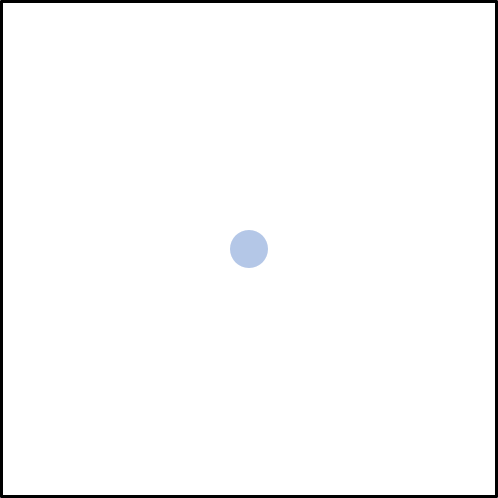
\includegraphics[width=\textwidth]{figs/rpm_1.png}
         \caption{}
     \end{subfigure}
     \hfill
     \begin{subfigure}[b]{0.24\textwidth}
         \centering
         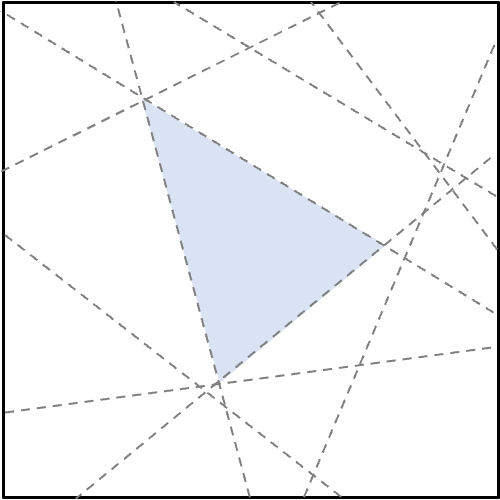
\includegraphics[width=\textwidth]{figs/rpm_2.png}
         \caption{}
     \end{subfigure}
     \hfill
     \begin{subfigure}[b]{0.24\textwidth}
         \centering
         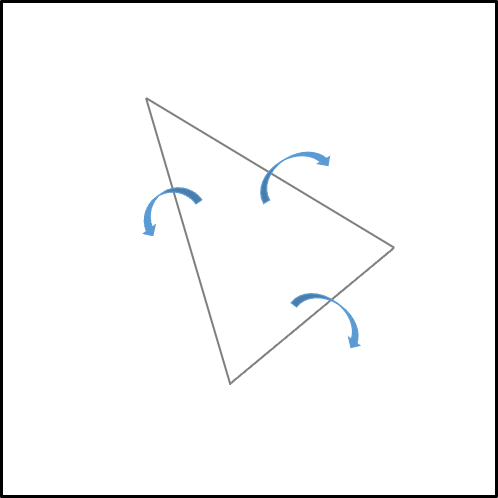
\includegraphics[width=\textwidth]{figs/rpm_3.png}
         \caption{}
     \end{subfigure}
     \hfill
     \begin{subfigure}[b]{0.24\textwidth}
         \centering
         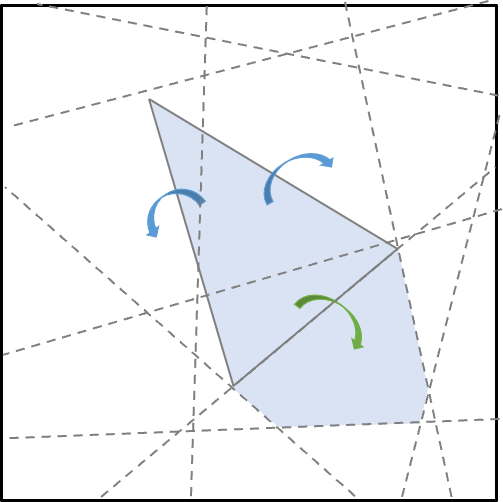
\includegraphics[width=\textwidth]{figs/rpm_4.png}
         \caption{}
     \end{subfigure}
        \caption{This figure illustrates the main steps of the RPM algorithm (Algorithm \ref{Algo:cell_enumeration}). (a) The algorithm is initialized with a point in the input space that is evaluated by the ReLU network to determine the activation pattern $\lambda$. (b) Then the polyhedron corresponding to $\lambda$ is computed using Algorithm \ref{Algo:ap_to_poly}. (c) Next, the essential constraints for the polyhedron, which in turn connect it to unexplored neighboring regions (indicated by blue arrows), are determined using Algorithm \ref{Algo:essential hrep}. (d) Then the activation pattern for a neighboring region (indicated by the green arrow) is found using Algorithm \ref{Algo:neighbor_ap}. The process then repeats by recursively exploring neighboring regions in this manner until the entire input set is explored.}
        \label{fig:alg_steps}
\end{figure*}

\subsection{Determining Neighboring Activation Patterns} \label{Neighbors}
Consider two neighboring polyhedra $P_k$ and $P_{k'}$ such that their shared face is identified by $\ba_\eta^\top \bx = b_\eta$ and $\ba_\eta^\top \bx \le b_\eta$ is an essential constraint for $P_k$, while $-\ba_\eta^\top \bx \le -b_\eta$ is an essential constraint for $P_{k'}$. We call $\ba_\eta^\top \bx \le b_\eta$ the neighbor constraint. Given the neuron activation pattern $\lambda$ for $P_k$, we next describe a procedure to find the activation pattern $\lambda'$ for $P_{k'}$, from which we can find the essential halfspace constraints from the procedure described in the previous section. This allows us to systematically generate all the activation patterns that are realizable by the network, and to obtain the polyhedra and affine maps associated with each of those activation patterns.  

Intuitively, to generate $\lambda_{k'}$ one ought to simply flip the activation of the neurons defining $\ba_\eta^\top \bx \le b_\eta$, and compute all the resulting new halfspace constraints from later layers in the network from (\ref{Eq:HalfspaceDef}). However, this intuitive procedure is incomplete because it does not correctly account for the influence that one neuron may have on other neurons in later layers. Flipping one neuron may lead to other neurons in later layers being flipped as well. To correctly determine the downstream effects of flipping a neuron, we provide a theorem for when neuron activations must be flipped.

\begin{theorem}[Neighboring Activation Patterns]
\label{thm: activation_flipping}
For a given region $P_k$, each neuron defines a hyperplane $\ba_{k,ij}^\top \bx = b_{k,ij}$, as given by (\ref{eq:normalize}). Suppose regions $P_k$ and $P_{k'}$ neighbor each other and are separated by $\ba_\eta^\top \bx = b_\eta$ where $P_{k} \subset \{\bx \mid \ba_\eta^\top \bx \le b_\eta \}$. Then,
\begin{enumerate}
    \item if $[\ba_{k,ij}^\top\quad  -b_{k,ij}] \neq \alpha[\ba_\eta^\top\quad -b_\eta]$ for some $\alpha \in \{0,1\}$, the activation of neuron $ij$ does not change, $\lambda_{k,ij} = \lambda_{k',ij}$.
    \item If $[\ba_{k,ij}^\top\quad  -b_{k,ij}] = \alpha[\ba_\eta^\top\quad -b_\eta]$ for some $\alpha \in \{0,1\}$, then $[\ba_{k',ij}^\top\quad  -b_{k',ij}] = \alpha[\ba_\eta^\top\quad -b_\eta]$ for some $\alpha \in \{-1,0\}$, and the activation $\lambda_{k',ij}$ should be set to ensure this holds.
\end{enumerate}
\end{theorem}

The proof for Theorem \ref{thm: activation_flipping} is in the Appendix. Then, the procedure to generate a neighboring activation pattern is defined in Algorithm \ref{Algo:neighbor_ap}. We present Algorithm \ref{Algo:neighbor_ap} in as simple a manner as possible, however, for a more efficient approach, one need not loop over all neurons in the network, but only those that meet condition 2) of Theorem \ref{thm: activation_flipping}.

% \begin{definition}[Type 1, 2, 3 neurons] \label{types}
% \textcolor{black}{Mac: Not formal enough, I think.  Let's discuss.} When identifying the activation pattern $\lambda'$ for a neighboring region $P'$ from a current region $P$, neurons whose halfspace constraints in $P$ define a non-empty boundary $P \cap P'$ are called \textit{Type 1}. Neurons with degenerate halfspace constraints in $P$, $\mathbf{0}^{\top} \bx \le b \ \forall \bx \in P$ where $b\ge 0$ are called \textit{Type 2}. All other neurons are \textit{Type 3}. 
% \end{definition}

% We find, in fact, that when flipping a neuron $\lambda_{(ij)}$ only Type 1 and Type 2 neurons in later layers $\lambbda_{kl}$, $k>i$, may be flipped as a result, according to the rules in the following theorem. \textcolor{black}{Mac: We need a formal theorem here, which is proved in the proof in the appendix.} 




\begin{algorithm}[!h]
\SetAlgoLined
\DontPrintSemicolon
 \KwIn{$\lambda_k$, $\mathbf{a}_\eta$, $b_\eta$, $\bTheta$}
 \KwOut{$\lambda_{k'}$}
 $\lambda_{k'} \leftarrow  \lambda_k$ \algorithmiccomment{Initialize neighbor region $\lambda$} \\
 
\For{$i = 1,\ldots,L-1$, $j = 1,\ldots,l_i$}{ 
% $\mathbf{a}_{ij},\ b_{ij} \leftarrow$ Equation \ref{eq:ab} \algorithmiccomment{$\lambda_{k',ij}$ hyperplane} \\
$\mathbf{a}_{k',ij},\ b_{k',ij} \leftarrow$ (\ref{eq:normalize}) \\
\uIf{$\mathbf{a}_{k',ij} = \mathbf{a}_\eta \quad \textbf{\upshape and}\quad b_{k',ij} = b_\eta$}
{$\lambda_{k',ij} \leftarrow \neg \lambda_{k,ij} $}
\uElseIf{$\mathbf{a}_{k',ij} = \mathbf{0} \quad \textbf{\upshape and}\quad b_{k',ij} = 0$}
{$\lambda_{k',ij} \leftarrow 0$}
}
\Return{$\lambda_{k'}$}
\caption{Neighboring Activation Pattern}
\label{Algo:neighbor_ap}
\end{algorithm}

% \begin{algorithm}[!h]
% \SetAlgoLined
% \DontPrintSemicolon
%  \KwIn{$\lambda_k$, $\mathbf{a}_\eta$, $b_\eta$, $\Theta$}
%  \KwOut{$\lambda_{k'}$}
%  $\lambda_{k'} \leftarrow  \lambda_k$ \algorithmiccomment{Initialize new $\lambda$ as old $\lambda$} \\
 
% \For{$i \in [1,\ldots,n-1]$, $j \in [1,\ldots,l_i]$}{ 
% \If{$ij \in$ \upshape Type 1  or $ij \in$ \upshape Type 2}{
% % $\mathbf{a}_{ij},\ b_{ij} \leftarrow$ Equation \ref{eq:ab} \algorithmiccomment{$\lambda_{k',ij}$ hyperplane} \\
% $\mathbf{a}_{ij},\ b_{ij} \leftarrow$ Equation \ref{eq:normalize} \\
% \uIf{$\mathbf{a}_{ij} = \mathbf{0} \quad \textbf{\upshape and}\quad b_{ij} < 0$}
% {$\lambda_{k',ij} \leftarrow \neg \lambda_{k,ij} $}
% \uElseIf{$\mathbf{a}_{ij} = \mathbf{a}_\eta \quad \textbf{\upshape and}\quad b_{ij} < b_\eta$}{$\lambda_{k',ij} \leftarrow \neg \lambda_{k,ij} $}
% \ElseIf{$\mathbf{a}_{ij} = -\mathbf{a}_\eta \quad \textbf{\upshape and}\quad b_{ij} < -b_\eta$}{$\lambda_{k',ij} \leftarrow \neg \lambda_{k,ij} $}
% }
% }
 
% \Return{$\lambda_{k'}$}
% \caption{Neighboring Activation Pattern}
% \label{Algo:neighbor_ap}
% \end{algorithm}

% where the preactivation value of a neuron as a function of the input is 
% \begin{align}
%     \hat{z}_{ij}(\bx) = \mathbf{W}_i \mathbf{z}_{i-1}(\bx) + \mathbf{b}_i.
% \end{align}
% The closure of the feasible set given by all such nonlinear constraints is the polyhedron $c$. Finding which neuron activations to flip when $\bx$ transitions from $c$ to $c'$ is equivalent to finding which nonlinear constraints must be flipped such that the resulting feasible set is $c'$. The distinction between the linear constraints given by (\ref{eq:constraints}) and the nonlinear constraints given by (\ref{eq:nonlinear}) is that the nonlinear constraint equations $\hat{z}_{ij}(\bx)$ hold for all inputs $\bx \in \mathbb{R}^{k_0}$, whereas the linear constraint parameters $\mathbf{a}_{ij}$ and $b_{ij}$ are valid only for $\bx \in c$. \textcolor{black}{mac: The above explanation is too vague to be useful.  How are they mathematically related  What is equal to what and under what conditions?  Best to just find a better notation that only uses $a_{ij}$.} 

% the set of points where a nonlinear constraint equation equals zero is restricted to hyperplanes, when in fact a nonlinear constraint equation can equal zero over full dimensional sets as well. This is illustrated by neurons associated with the degenerate linear constraint $\mathbf{0}\cdot \bx = 0 \ \forall \bx \in c$. 

% Informally, flipping the sense of a nonlinear constraint flips which side of the constraint boundary is feasible. We seek to flip the sense of nonlinear constraints if doing so leads to feasibility in the $c'$. 
% The feasible set given by the intersection of each hidden neuron nonlinear constraint is exactly the polyhedron given by Equation (\ref{eq:constraints}). Moreover, the nonlinear constraints defined by an activation pattern are equivalent to the linear constraints from Equation (\ref{eq:constraints}) for $\bx \in c$. 
% Given the activation pattern of a ReLU network, neurons are associated with linear constraints by (\ref{eq:constraints}). These constraints are local in the sense that they are only valid for $\bx \in c$. But more generally, an activation pattern describes nonlinear constraints that hold for all inputs. For neuron $j$ in layer $i$
% \begin{align}
% \begin{cases}
% \hat{z}_{i,j}(\bx) \ge 0\ \ \text{if}\   \ AP_{i,j} = 1 \\
% \hat{z}_{i,j}(\bx) \le 0\ \ \text{if}\   \ AP_{i,j} = 0
% \end{cases}.
%  \label{eq:nonlinear}
% \end{align}
% For example, a nonlinear constraint in layer two is
% \begin{align}
% \hat{z}_{2,j}(\bx) =
% \begin{cases}
% \tilde{\mathbf{W}}_2[j,:]\sigma(\tilde{\mathbf{W}}_1 \tilde{\bx}) \ge 0 \ \ AP_{i,j} = 1 \\
%  \tilde{\mathbf{W}}_2[j,:]\sigma(\tilde{\mathbf{W}}_1 \tilde{\bx}) \le 0 \ \ AP_{i,j} = 0.
% \end{cases}
% \end{align}

% A nonlinear constraint is active when $\hat{z}_{i,j}(\bx) = 0$. Note that this is different than the notion of a ReLU being active or inactive. The region for which a nonlinear constraint is active is not restricted to be a lower dimensional facet of a cell. For instance Type 2 constraints are active over an entire cell.

% Since interior inputs from the original cell should be infeasible for the neighbor cell constraints, a naive approach to determining the neighboring activation pattern is to simply flip the neuron activation for each Type 1 neuron. This is the right intuition, but an incomplete approach. The intuition this draws on is that the sense of a nonlinear constraint should be flipped if the constraint boundary is coincident with the shared boundary between the original and neighbor cell. 

% Since we want to flip the sense of a nonlinear constraint if its constraint boundary is coincident with the shared neighbor boundary, it is useful to characterize where the constraints are active. 

% In addition, we must not flip the sense of nonlinear constraints associated with Type 2 neurons. Lastly, we may need to flip the sense of some constraints associated with Type 3 neurons.

% Equation \ref{g1} is true by construction of the Type 1 set. If Equation \ref{g2} were not true that would imply that the associated halfspace constraint for a Type 2 neuron would be equal to the halfspace constraint for a Type 1 neuron which is a contradiction according to the construction of the Type 1 and Type 2 sets. Thus Equation \ref{g2} is true. Equation \ref{g3} is true because the degenerate halfspace constraints associated with these neurons indicate that Type 3 neurons always evaluate to 0 on the parent cell (of which the shared boundary is included).

% \begin{enumerate}
%   \item If the updated linear constraint generated by a Type 1 neuron is $\mathbf{0} \cdot \bx \le 0$, then the updated activation for that neuron is $0$ (regardless of whether it was 1 or 0 in the original cell) (Figure \ref{fig:constraints}c). Otherwise, the activation is flipped (Figure \ref{fig:constraints}b).
%   \item If the updated linear constraint generated by a Type 2 neuron is equal and opposite to the original essential constraint (defined by Type 1 neurons), then the activation is flipped from a 0 to a 1 (Figure \ref{fig:constraints}d). Otherwise, it remains 0 (Figure \ref{fig:constraints}e).
% \end{enumerate}
% Note that since linear constraints are unchanged when multiplied by a scalar, the linear constraints from (\ref{eq:constraints}) must be normalized to perform the comparison in rule 2.

% We know that Type 1 nonlinear constraints are active at the boundary. Once past the boundary into the neighbor cell, these constraints can become inactive, in which case the sense of the constraint is flipped. Or they can remain active, in which case the constraint is not flipped. This corresponds to the constraint being active over the entire neighbor cell, and thus the neuron is a Type 3 neuron for the neighbor cell.

% Also, we know there exists some $\delta$ we can go past the shared boundary, into the neighbor cell, where the sense of the Type 2 nonlinear constrains do not flip. This is because each $g_{ij}(x)$ is a continuous function. Thus, the sense of Type 2 constraints remains the same.

% Like the Type 1 constraints, the constraint boundary for Type 3 neurons may lie coincident with the shared boundary. If coincident with the shared boundary, we must flip the sense of the nonlinear constraint. Otherwise we do not flip, as the original constraint is still active. Thus, the sense of a Type 3 nonlinear constraint will flip if and only if flipping the new halfspace constraint associated with it (after flipping necessary neurons in previous layers and re-computing the halfspace constraints) equals the new, flipped, Type 1 constraints.


%%%%%%%%%%%%%%%%%%%%%%%%%%%%%%%%%%%%%%%%%%%%%%%%%%
%%%%%%%%%%%%%%%%%%%%%%%%%%%%%%%%%%%%%%%%%%%%%%%%%%
\subsection{Reachable Polyhedral Marching} \label{Cell Enumeration}
% \begin{figure*}
%     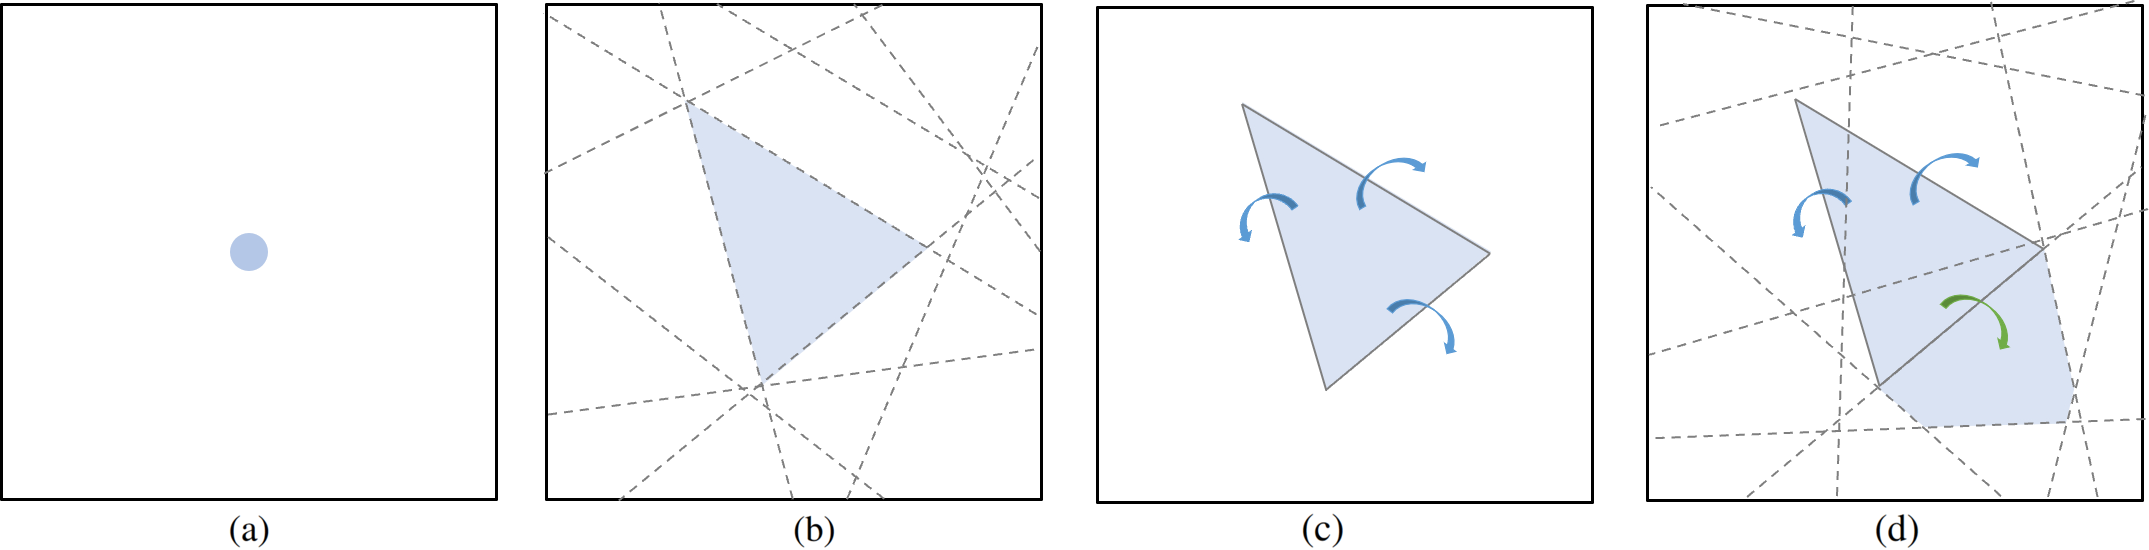
\includegraphics[width=\textwidth]{figs/rpm_fig1.png}
%     \centering
%     \caption{When transitioning from region $P_k$ to region $P_{k'}$, some neuron activations must flip to ensure their associated halfspace constraints (as given by (REF)) are valid for $P_{k'}$. In (a), two neighboring regions $P_k$ and $P_{k'}$ are shown. Constraint $1$ is the neighbor constraint $\ba_\eta^\top \bx = b_\eta$ and is shared by both regions. Constraint $2$ is different in $P_k$ and $P_{k'}$, but induced by the same neuron. We know from (REF) that only those neurons whose associated halfspace constraints in $P_k$ are scalar multiples of the neighbor constraint may need to flipped, and that in $P_{k'}$ their updated halfspace constraints will remain scalar multiples of the neighbor constraint. To flip the correct neuron activations, Algorithm REF iterates through each neuron and initially assumes each activation is the same in $P_{k'}$ as it was in $P_k$. From this assumed activation, if a neuron's constraint is a scalar multiple of the neighbor constraint then we check whether it is a feasible constraint for $P_{k'}$. Given the neighbor constraint $\ba_\eta^\top \bx \le b_\eta$ shown in blue, (b) and (e) illustrate feasible constraints while (c) and (d) do not (and therefore require the activation to be flipped). Finally, it is possible for a candidate neuron's constraint to be $\mathbf{0}^\top \bx \le b$, in which case it is feasible if $b \ge 0$ and flipped otherwise. These situations are the basis for the neuron activation flipping rules in Algorithm REF.
%     % \textcolor{black}{Mac: This is too confusing to be understood by the reader, and it's not referred to enough in the text. We should really leverage this figure in the explanation to tell the story of the flipping rules.} The activation of a neuron in $P_k$ defines a nonlinear constraint $\mathbf{a}(\bx)^\top \bx \le b(\bx)$ which may remain valid in $P_{k'}$, or may need to be flipped. Type 3 neurons need not be flipped, while Type 1 ((a)-(c)) and Type 2 ((d)-(f)) neurons may need to be flipped. Let $\mathbf{a}(\bx)^\top \bx < b(\bx)$ be shown in green, $\mathbf{a}(\bx)^\top \bx > b(\bx)$ in red, and the special case of $\mathbf{a}(\bx) = \mathbf{0}$ in blue. To determine a neuron activation in $P'$, we first determine which scenario ((a)-(f)) applies. Clearly, for the cases illustrated by (a) and (d), the neuron activation must be flipped to ensure it defines a valid constraint in $P_{k'}$. However, for the remaining scenarios, the rules for flipping neuron activations are more nuanced. A full discussion of the neuron flipping rules is given in the Appendix.
%     }
%     \label{fig:constraints}
% \end{figure*}



Building on Algorithms \ref{Algo:essential hrep} \& \ref{Algo:neighbor_ap}, we now define our main algorithm, Reachable Polyhedral Marching (RPM) in Algorithm \ref{Algo:cell_enumeration} for explicitly enumerating all polyhedra in the input space of a ReLU network, resulting in the explicit PWA representation. 
First we start with a polyhedral set of inputs we would like to enumerate affine regions over.
This set of inputs can also be $\mathbb{R}^n$, but in most applications it makes sense to consider a bounded set of inputs.
Then, we find an initial point within the input set and evaluate the network to find the activation pattern. 
% Note, this initial point should lie in the interior of a polyhedral region, not on the boundary. 
From this, the essential H-representation is found using Algorithm \ref{Algo:essential hrep}. 
For each essential constraint we generate a neighboring activation pattern using Algorithm \ref{Algo:neighbor_ap}. 
The process then repeats with each new neighboring activation pattern being added to a working set. 
For a given starting polyhedron each neighbor polyhedron is enumerated, and since all polyhedra are connected via neighbors, Algorithm \ref{Algo:cell_enumeration} is guaranteed to enumerate every polyhedron in the input space. 
Figure \ref{fig:alg_steps} illustrates the steps of RPM and Figure \ref{fig:cell_enum} shows the result of applying Algorithm \ref{Algo:cell_enumeration} to a ReLU network trained to model a quadratic function.

The bulk of the computation for Algorithm \ref{Algo:cell_enumeration} is dedicated to solving the LPs needed to retrieve the essential H-representation for each polyhedron (Algorithm \ref{Algo:essential hrep}).
In the worst case, for each polyhedron in the input space, Algorithm \ref{Algo:cell_enumeration} solves an LP for each neuron in the network. 
As noted in Section \ref{sec:relu_networks}, the number of polyhedra for the algorithm to explore scales according to $\mathcal{O}(N^n)$ where $N$ is the number of neurons and $n$ is the dimension of the input space.
Thus, in the worst case, the number of LPs solved by the algorithm scales according to $\mathcal{O}(N^{2n})$.
This exponential complexity in the input dimension is unsurprising and is inherent to the exact analysis of ReLU neural networks \cite{reluplex}.


\begin{algorithm}
\SetAlgoLined
\DontPrintSemicolon
 \KwIn{$\lambda_{0}$, $\bTheta$}
 \KwOut{Explicit PWA representation}
 PWA = $\emptyset$;  visited = $\emptyset$ \\
 working set = \{$\lambda_0$\} \\
 \While{$\text{\upshape working set} \neq \emptyset$}{
 $\lambda_k \leftarrow$ pop next $\lambda$ off working set \\
 $\bA_k, \bb_k \leftarrow$ Algorithm \ref{Algo:essential hrep} \algorithmiccomment{Retrieve essential H-rep} \\
 $\mathbf{C}_k,\ \mathbf{d}_k \leftarrow$ (\ref{eq:CdDef}) \algorithmiccomment{Retrieve affine map} \\
 push ($\bA_k, \bb_k, \bC_k, \bd_k$) onto PWA \\
 \For(\algorithmiccomment{For each neighbor}){$\mathbf{a}_{k,i}, b_{k,i} \in \bA_k, \bb_k$}{
 $\lambda_{k'} \leftarrow$ Algorithm \ref{Algo:neighbor_ap} \algorithmiccomment{$\ba_\eta, b_\eta = \ba_{k,i}, b_{k,i}$} \\
 \If{$\lambda_{k'} \notin \text{\upshape visited} \cup \text{\upshape working set}$}{
 push $\lambda_{k'}$ onto working set \\
 }
 }
 push $\lambda_k$ onto visited\\
 }
 \Return{\text{\upshape PWA}}
 \caption{Reachable Polyhedral Marching}
 \label{Algo:cell_enumeration}
\end{algorithm}

%%%%%%%%%%%%%%%%%%%%%%%%%%
\section{Reachability} 
%%%%%%%%%%%%%%%%%%%%%%%%%
\label{Sec:Reachability}
\subsection{Forward Reachability} \label{Forward}
The forward reachable set of a PWA function over some input set is simply the union over the forward reachable sets of each polyhedron comprising the input set. The image of a polyhedron under an affine map is
\begin{align}
    P_{image} = \{\by \mid \by=\mathbf{Cx}+\mathbf{d},\quad \mathbf{Ax} \le \mathbf{b}\}. \label{eq:forward reach}
\end{align}
For invertible $\mathbf{C}$, the H-representation of the image is
\begin{align}
    P_{image} = \{\by \mid \mathbf{AC}^{-1}\by \le \mathbf{b} + \mathbf{AC}^{-1} \mathbf{d}\}. \label{eq:image}
\end{align}
In the case the affine map is not invertible, more general polyhedral projection methods such as block elimination, Fourier-Motzkin elimination, or parametric linear programming can compute the H-representation of the image \cite{cdd_manual, mpLP}. 
Our implementation uses the block elimination projection in the case of a non-invertible affine map \cite{cdd}.

Our RPM algorithm is used to perform forward reachability as follows. We first specify a polyhedral input set whose image through the ReLU network we want to compute.  This is a set over which to perform the RPM algorithm. For each activation pattern $\lambda_k$ we also compute the image of $(\bA_k, \bb_k)$ under the map $\by = \mathbf{C}_k\bx + \mathbf{d}_k$. To do this, an additional line is introduced between lines 9 and 10 of Algorithm \ref{Algo:cell_enumeration}
\begin{align}
    (\bA_k, \bd_k)_{forward} \leftarrow \text{project}(\bA_k, \bd_k, \mathbf{C}_k, \mathbf{d}_k)
\end{align}
where $\text{project}(\bA, \bb, \bC, \bd)$ applies (\ref{eq:image}) if $\mathbf{C}$ invertible and block elimination on (\ref{eq:forward reach}) otherwise.


%%%%%%%%%%%%%%%%%%%%%%%%%%%%%%%%%%%%%%%%%%%%%%%%%%
%%%%%%%%%%%%%%%%%%%%%%%%%%%%%%%%%%%%%%%%%%%%%%%%%%
\subsection{Backward Reachability} \label{Backward}
The preimage of a polyhedron under an affine map is
\begin{subequations}
    \begin{align}
        P_{pre} &= \{\bx \mid \by=\mathbf{Cx}+\mathbf{d},\quad \mathbf{Ay} \le \mathbf{b}\} \\
        &= \{\bx \mid \mathbf{ACx} \le \mathbf{b}-\mathbf{Ad}\}. \label{eq:backward reach}
    \end{align}
\end{subequations}
Like forward reachability, performing backward reachability only requires a small modification to Algorithm \ref{Algo:cell_enumeration}. We first specify a polyhedral output set whose preimage we would like to compute.  For each activation pattern $\lambda_k$, we then compute the intersection of the preimage of the given output set under the map $\mathbf{C}_k\bx + \mathbf{d}_k$ with $P_k$ (the polyhedron for which the affine map is valid). Two additional lines are thus introduced between lines 9 and 10 of Algorithm \ref{Algo:cell_enumeration}
\begin{subequations}
    \begin{gather}
    P_{pre} \leftarrow \text{Equation}\ \ref{eq:backward reach} \label{eq:p_in} \\
    (\bA_k, \bb_k)_{backward} \leftarrow P_k \cap P_{pre}. \label{eq:h_back}
    \end{gather}
\end{subequations}
Multiple backward reachable sets can be solved for simultaneously at the added cost of repeating (\ref{eq:p_in}) and (\ref{eq:h_back}) for each output set argument to Algorithm \ref{Algo:cell_enumeration}.

Finally, we address the issue of finding $t$-step forward and backward reachable sets for a dynamical system represented as a neural network, $\bx_{t+1} = F(\bx)$.
For a ReLU network that is applied iteratively over $t$ time steps, $\bx_t = F \circ \cdots \circ F(\bx_0)$.
Thus, we can concatenate the ReLU network $F$ with itself $t$ times, forming one larger network representing a $t$-step update.
If the original network $F(\bx)$ has $r$ hidden layer neurons and $N$ layers, the concatenated network has $tr$ neurons and $t(N-1) + 1$ layers.  
We then simply perform RPM for forward or backward reachability on the concatenated network.
Thus, computing a $t$-step reachable set is as expensive as computing a $1$-step reachable set for a network with $t$ times the depth.

%%%%%%%%%%%%%%%%%%%%%%%%%%%%%%%%%%%
% \section{Control Invariant Sets}
%%%%%%%%%%%%%%%%%%%%%%%%%%%%%%%%%%%
% \label{Sec:Invariant}
% In this section we discuss a strategy for computing control invariant sets once we have the PWA representation of a dynamical system $\bx_{t+1} = F(\bx_t, \mathbf{u}_t)$.
First, we note that for some state transition functions $F$, there may not exist a control invariant set.
Existence of such a set depends on the state domain $\mathcal{X}$ and the set of admissible control inputs $\mathcal{U}$, as well as the specific effect of control inputs on the state transitions given by $F$.
A common strategy for computing control invariant sets is to compute the following recursion using backward reachability,
\begin{subequations}
\begin{gather}
    X_0 = \mathcal{X} \\
    X_{i+1} = \{\bx \mid F(\bx,\mathbf{u}) \in X_{i}, \mathbf{u} \in \mathcal{U} \}
\end{gather}
\end{subequations}
for a compact polyhedral state domain $\mathcal{X}$ and set of admissible inputs $\mathcal{U}$. 
If $X_{i+1} = X_i$, then $X_i$ is a control invariant set. 
This recursion for computing control invariant sets is implemented in MPT3 specifically for PWA dynamical systems \cite{MPT3}.
% \textcolor{blue}{In this section we reiterate the main results from \cite{pwa_lygeros} for computing robust control invariant sets of discrete-time PWA dynamical systems.}
% Given a dynamical system represented as a ReLU network we can use Algorithm \ref{Algo:cell_enumeration} to retrieve the explicitly defined PWA system and then use the following techniques to compute robust control invariant sets.
% \textcolor{blue}{This approach is the first general framework for computing robust control invariant sets for dynamical systems defined by ReLU networks.}
% We first define a few useful terms.
% \begin{definition}[Fixed Point] \label{def:fixed_point}
% A vector $\bx \in \mathbb{R}^n$ is a fixed point of the function $f(\bx): \mathbb{R}^n \rightarrow \mathbb{R}^n$ if $f(\bx) = \bx$.
% \end{definition}

% \begin{definition}[Invariant Set] \label{def:invariant}
% A (forward) invariant set of an autonomous dynamical system $\bx^+ = f(\bx)$ is a set of states for which any trajectory starting in the invariant set remains in the set for all time.
% \end{definition}

% Building on these definitions, a set of states is robust control invariant if there always exists a control input such that the subsequent state under the dynamics will remain in the set under all possible disturbance values. Computing robust invariant sets for autonomous systems or control invariant sets for deterministic controlled systems are special instances of this general problem. We now summarize the main results from \cite{pwa_lygeros}.

% Suppose we have the  system model
% \begin{subequations}
% \begin{align}
%     \bx^{+} &= f(\bx, \mathbf{u}, \mathbf{w}) \\
%     (\bx,\mathbf{u}) &\in Y \subset \mathcal{X} \times \mathcal{U} \\
%     \mathbf{w} &\in W(\bx,\mathbf{u}) \subset \mathcal{W}
% \end{align}
% \end{subequations}
% where $f$ is PWA, $\mathcal{X} = \mathbb{R}^n$, $\mathcal{U} = \mathbb{R}^m$, and $\mathcal{W} = \mathbb{R}^p$. We define the set of admissible state, control, and disturbance triples as
% \begin{align}
%     \mathcal{\gamma} = \{(\bx,\mathbf{u},\mathbf{w}) \mid (\bx,\mathbf{u})\in Y,\ \mathbf{w}\in W(\bx,\mathbf{u}) \}.
% \end{align}
% It follows that the set of admissible inputs and states are
% \begin{subequations}
% \begin{align}
%     U(\bx) &= \{\mathbf{u} \mid (\bx,\mathbf{u}) \in Y \} \\
%     X &= \{\bx \mid \exists \mathbf{u}\ \text{s.t.}\ (\bx,\mathbf{u}) \in Y \} = Proj_{\mathcal{X}}(Y).
% \end{align}
% \end{subequations}
% Additionally, let $X_f$ represent a target robust control invariant set. The general strategy is to start with $X_f$ and step backwards in time to compute set of states that lead to $X_f$. We can then iterate upon this until convergence or as long our computational resources allow.
% \begin{definition}[Predecessor Set]
% Given a set $\Omega \subset \mathcal{X}$, the predecessor set $Pre(\Omega)$ is the set of states for which there exists an admissible input such that, for all allowable disturbances, the successor state is in $\Omega$, i.e.,
% \begin{multline}
%  Pre(\Omega) :=  \\
%     \scalemath{0.95}{\{\bx \mid \exists \mathbf{u} \in U(\bx)\ s.t.\ f(\bx,\mathbf{u},\mathbf{w}) \in \Omega \ \forall \mathbf{w} \in W(\bx,\mathbf{u}) \}}.
% \end{multline}
% \end{definition}
% Let $X_t$ denote the $t$-step predecessor set to $X_f$. That is,
% \begin{subequations}
% \begin{align}
%     X_0 &= X_f \\
%     X_{t+1} &= Pre(X_t).
% \end{align}
% \end{subequations}
% A set $S \subset X$ is robust control invariant if for any $\bx\in S$ there exists a $\mathbf{u} \in U(\bx)$ such that $f(\bx,\mathbf{u},\mathbf{w}) \in S$ for all $\mathbf{w} \in W(\bx,\mathbf{u})$. It is known that $X_t$ is robust control invariant for all $t$ if and only if $X_f$ is robust control invariant. Thus, the problem of computing robust control invariant sets involves finding an initial robust control invariant set $X_f$ and then computing predecessor sets $X_t$. For PWA systems it is often advantageous to compute $X_f$ for an affine region of $f$ since computing robust control invariant sets is much easier for affine systems than for nonlinear systems. 

% Next we present the main result of \cite{pwa_lygeros} which leads to Algorithm \ref{Algo:invariant_set} for computing robust control invariant sets. Define the set of robust state and control tuples and the preimage operation as
% \begin{subequations}
% \begin{align}
%     \Sigma &:= \scalemath{0.96}{\{(\bx,\mathbf{u}) \in Y \mid f(\bx,\mathbf{u},\mathbf{w}) \in \Omega \ \forall \mathbf{w} \in W(\bx,\mathbf{u}) \}} \\
%     \Phi &:= \scalemath{0.96}{f^{-1}(\Omega) = \{(\bx,\mathbf{u},\mathbf{w}) \mid f(\bx,\mathbf{u},\mathbf{w}) \in \Omega \}}.
% \end{align}
% \end{subequations}
% Then the main result from \cite{pwa_lygeros} is
% \begin{subequations}
% \begin{align}
%     Pre(\Omega) &= Proj_{\mathcal{X}}(\Sigma) \\
%     \Sigma &= Y\ \backslash\ Proj_{\mathcal{X} \times \mathcal{U}}(\mathcal{\gamma}\ \backslash\ \Phi)
% \end{align}
% \end{subequations}
% where $A \backslash B$ is the set difference between sets $A$ and $B$. Algorithm \ref{Algo:invariant_set} outlines the process for computing the $i$-step predecessor set of a seed robust control invariant set $X_0$. If $\mathcal{\gamma}$ and $X_f$ are each a union of polyhedra then each $X_t$ will be a union of polyhedra and $\Phi$ can be computed by adapting the backward reachability algorithm from Section \ref{Sec:Reachability} and standard computational geometry methods can be used to perform the necessary set projections and differences. Algorithm \ref{Algo:invariant_set} is very general and faster algorithms exist for special cases, such as if the disturbance is additive \cite{robust_step}.

% \begin{algorithm}
% \SetAlgoLined
% \DontPrintSemicolon
%  \KwIn{$\mathcal{\gamma}$, $X_0$}
%  \KwOut{$X_T$}
%  Compute the projection $Y = Proj_{\mathcal{X} \times \mathcal{U}}(\mathcal{\gamma})$ \\
%  \For{$t = 1,\ldots,T$}{
%  Compute the preimage $\Phi_t = f^{-1}(X_{t-1})$ \\
%  Compute the set difference $\Delta_t = \mathcal{\gamma}\ \backslash \ \Phi_t$ \\
%  Compute the projection $\Psi_t = Proj_{\mathcal{X} \times \mathcal{U}}(\Delta_t)$ \\
%  Compute the set difference $\Sigma_t = Y\ \backslash \ \Psi_t$ \\
%  Compute the projection $X_t = Proj_{\mathcal{X}}(\Sigma_t)$ \\
%  }
%  \Return{$X_T$}
%  \caption{Robust Control Invariant Set \cite{pwa_lygeros}}
%  \label{Algo:invariant_set}
% \end{algorithm}

%%%%%%%%%%%%%%%%%%%%%%%%%%%%%%%%%%%%%%%%%%
\section{Invariant Sets}
%%%%%%%%%%%%%%%%%%%%%%%%%%%%%%%%%%%%%%%%%%
\label{Sec:ROA}
\subsection{Control Invariant Sets}
In this subsection we discuss a strategy for computing control invariant sets once we have the PWA representation of a dynamical system $\bx_{t+1} = F(\bx_t, \mathbf{u}_t)$.
This strategy for computing control invariant sets is implemented in MPT3 specifically for PWA dynamical systems \cite{MPT3}.
First, we note that for some state transition functions $F$, there may not exist a control invariant set.
Existence depends on the state domain $\mathcal{X}$ and the set of admissible control inputs $\mathcal{U}$, as well as the effect of control inputs on the state transitions given by $F$.
If a control invariant set exists, it can be computed via the following recursion which uses backward reachability,
\begin{subequations}
\begin{gather}
    X_0 = \mathcal{X} \\
    X_{i+1} = \{\bx \mid F(\bx,\mathbf{u}) \in X_{i}, \mathbf{u} \in \mathcal{U} \},
\end{gather}
\end{subequations}
for a compact polyhedral state domain $\mathcal{X}$ and set of admissible inputs $\mathcal{U}$. 
If $X_{i+1} = X_i$, then $X_i$ is control invariant. 




\subsection{Regions of Attraction}
% In Section \ref{Sec:Invariant} we gave a general overview of existing results for computing robust control invariant sets of PWA dynamical systems that we can apply to ReLU networks after computing the explicitly defined PWA representation using Algorithm \ref{Algo:cell_enumeration}. 
In this subsection we consider the problem of computing invariant ROAs given a ReLU network that represents an autonomous dynamical system $\bx_{t+1} = F(\bx_t)$. 
One of the most common goals in designing a control policy is to stabilize the system around some equilibrium.
By identifying a ROA, we are identifying a set of states which is stabilized.
% A common goal in the analysis of nonlinear dynamical systems is to identify the maximal set of states that is both a ROA and an invariant set. 
% We define a ROA as follows,
% \begin{definition}[Region of Attraction] \label{def:ROA}
% A region of attraction (ROA) of an autonomous dynamical system $\bx^+ = f(\bx)$ is a set of states that asymptotically converge to a stable fixed point $\bx_{fp}$. The set of \textit{all} states that asymptotically converge to a stable fixed point is the maximal ROA, i.e. $\text{ROA}_{max} = \{ \bx \mid \lim_{t\rightarrow \infty} f(\bx) = \bx_{fp} \}$. 
% \end{definition}

% Note that under our definition, a ROA need not be an invariant set (although the maximal ROA is invariant), but since our approach uses seed ROAs that are also invariant sets, as we grow the ROA backwards in time it remains an invariant set. 
The strategy we use to compute ROAs is as follows.
We first use RPM to enumerate each affine region of $F$ and within each region check for the existence of a stable fixed point.
If one is found, we then compute a small `seed ROA' around this equilibrium. 
Then we use backward reachability to find the $t$-step backward reachable set of the seed ROA, which itself is guaranteed to be an ROA (see \cite{pwa_lygeros}). 
The volume of the resulting ROA grows as more backward reachability steps are taken. Thus, the maximal ROA is better approximated by using more backward reachability steps.

In the following subsections we detail the procedure for finding fixed points, checking whether they are stable equilibria, and computing seed ROAs. 
We also describe how the computation of the ROA can be accelerated by exploiting the connected walk of RPM, and under what conditions this accelerated method captures the same result as the original method.
Finally, as with control invariant sets, there are some dynamical systems for which no ROA exists.
However, in our outlined procedure, the time taken to find fixed points (if they exist) is a small fraction of the time taken to find the ROA through backward reachability.
Thus, verifying that no ROA exists can be accomplished with relative ease (compared to verifying that no control invariant set exists, for example).
% Here we consider computing, via backward reachability, ROAs of ReLU networks that model the discrete-time dynamics of an autonomous system. 

\subsubsection{Finding Fixed Points}
To find fixed points of a ReLU network we use RPM to solve for the explicit PWA representation and for each region $k$ solve the following system of equations for $\bx$.
\begin{align}
    \mathbf{C}_k\bx + \mathbf{d}_k &= \bx \label{eq:fp}
\end{align}
We consider $\bx$ a fixed point if it is the unique solution of (\ref{eq:fp}) and lies on the interior of $P_k$. 
% We do not consider the case of non-unique solutions. 
A fixed point in $P_k$ is a stable equilibrium if $\mathbf{C}_k$ is a stable dynamics matrix. 
That is, if the eigenvalues of $\mathbf{C}_k$ have magnitude strictly less than one.
When all eigenvalues have magnitude strictly less than one, trajectories near the fixed point will asymptotically converge.

\subsubsection{Finding Seed ROAs} \label{seed}
For our backward reachability algorithm we require a polyhedral seed ROA to start from. Once a stable fixed point is located we translate the corresponding affine system to a linear one via a coordinate transformation. We can then use existing techniques for computing invariant polyhedral ROAs of stable linear systems \cite{hennet1995discrete}. 
Once a polyhedral ROA is found it can be scaled it up or down to ensure it is a subset of the polyhedron for which the local affine system is valid.
Then, it is well known that the backward reachable set of an invariant set is also an invariant set \cite{pwa_lygeros}.
Thus by finding the backward reachable set of the seed ROA, we grow the ROA.
% To see why this is the case it suffices to show that an invariant set is a subset of its preimage, which can be easily shown via a proof by contradiction.
% Thus, the preimage of the seed ROA will also be an ROA.
% In fact, these results extend more generally to robust control invariant sets, however finding seed robust control invariant sets is more challenging.}

\subsection{An Accelerated Procedure} \label{sec:homeo}
The backward reachability algorithm as previously presented can be made more efficient if RPM is restricted to only enumerated a connected backward reachable set.
Knowing that the fixed point $\bx_{eq}$ must be in the ROA, initializing RPM at the fixed point, and then only enumerating a connected backward reachable set of the seed ROA can significantly reduce the computation time.
In this case, we can alter the backward reachability algorithm to only add neighbor polyhedra to the working set if they are neighbors of a polyhedron known to be in the backward reachable set. 
% When initialized within the connected preimage, this procedure restricts the polyhedra RPM has to enumerate, leading to a substantial reduction in the compute time. 

The resulting set of states found by this procedure still converges to the equilibrium, but since we may not be computing the entire backward reachable set of the seed ROA, it may not be an invariant set.
Next we consider sufficient conditions for this accelerated procedure to still produce an ROA which is an invariant set.

It is known that the backward reachable set of a connected set will also be connected if the function mapping between the input and output spaces is a homeomorphism.
\begin{definition}[Homeomorphism] \label{def:homeo}
A function $f: \mathcal{X} \rightarrow \mathcal{Y}$ between two metric spaces is a homeomorphism if (i) $f$ is bijective, (ii) $f$ is continuous, (iii) $f^{-1}$ is continuous.
Furthermore, the composition of homeomorphisms is also a homeomorphism.
\end{definition}
PWA homeomorphic conditions are given in \cite{homeo2}.
\begin{theorem}[Homeomorphic PWA Functions \cite{homeo2}]
For affine maps $\mathbf{C}_k\bx + \mathbf{d}_k$ of regions $P_k \in \mathcal{P}$, let $\mathbf{C}[r]$ denote the matrix consisting of the first $r$ rows and columns of $\mathbf{C}$. If for each $r = 1, \ldots, n$,
\begin{align}
   \text{sgn det}(\mathbf{C}_k[r]) = \sigma_r \quad \forall k
\end{align}
where $\sigma_r \neq 0$ and sgn det() is the sign of the determinant, then the PWA function is a homeomorphism. 
% That is, all minor determinants of a given order must have the same sign across all affine map matrices.
\end{theorem}
Note that all $\mathbf{C}_k$ nonsingular is a necessary but insufficient condition. 
This theorem gives us a simple way to check whether a ReLU network is a homeomorphism once we have obtained the explicitly defined PWA function. 

Thus, if the ReLU network defining the dynamical system is a homeomorphism, then restricting RPM to enumerate a connected backward reachable set of the seed ROA results in no loss of generality and the set obtained remains invariant.
In our examples we explore the effect of this accelerated procedure and show that it can lead to dramatic decreases in computation time.
The computation time saved is roughly the ratio between the number of polyhedra in the connected backward reachable set and the number of polyhedra over the entire state domain $\mathcal{X}$.
Depending on the definition of the state domain, this ratio can be quite extreme.

Our method of decomposing ReLU networks into their explicit PWA representations using RPM and checking the homeomorphism condition is, to the best of our knowledge, the first approach for determining the invertibility of an arbitrary ReLU network. 
% We emphasize that it is not immediately obvious that ReLU networks can be homeomorphisms because, as the authors of \cite{topology} note, the ReLU activation itself is not homeomorphic and layer weight matrices often map between spaces of different dimension. But even though the equation of a ReLU network may not look homeomorphic, the underlying PWA function may still be homeomorphic. 
This procedure for checking invertibility may find use beyond the problems studied in this paper, like in training normalizing flow models~\cite{papamakarios2021normalizing}.

% \textcolor{black}{Lastly, although the homeomorphic condition may not always hold, we think this accelerated procedure is still worthwhile as it still allows a user to find a set of states which are stabilized (even though whether the set is invariant is unknown).
% We take this view in Section \ref{Taxinet} where we analyze the stabilizing properties of a learned policy, where the closed-loop PWA dynamics has orders of magnitude many more affine regions than other numerical examples explored in the literature.}
% Finally, we are not aware of any other work that checks and uses the homeomorphism conditions to accelerate PWA backward reachability, but we have found that utilizing this information can result in significant speedups, as discussed in Section \ref{sec:vanderpol}.

% Somewhat surprisingly, we find the homeomorphic property holds for many of the learned dynamical systems used in Section \ref{Sec:Examples} without special modifications to the training procedure. 
% Because of this, we think investigation into learning homeomorphic neural networks is a promising direction for future research. 


%%%%%%%%%%%%%%%%%%%%
\section{Examples} 
%%%%%%%%%%%%%%%%%%%%
\label{Sec:Examples}
All examples are run on a desktop computer with AMD Ryzen 5 5600X 3.7 GHz 6-Core processor and 16GB of RAM.
Our implementation uses the GLPK open-source LP solver and the JuMP optimization package \cite{DunningHuchetteLubin2017}. 
The polyhedron coloring in plots is random.

% \textcolor{black}{
% For each example we list the computation time.
% Although the computation times can grow large, we emphasize that our approach is the first general-purpose method for finding invariant sets and regions of attraction for dynamical systems defined as ReLU networks.
% Furthermore, from the examples it is clear that our approach of leveraging the homeomorphic property allows us to solve otherwise intractable problems.}

Given that answering queries about exact reachable sets of ReLU neural networks is NP-complete \cite{reluplex}, the application of the methods presented in this paper is constrained by (i) the size of the neural network to analyze and (ii) the properties one wishes to verify.
When only a single-step reachability computation is needed, as in verifying open-loop safety properties of a learned policy, the ReLU networks can be moderately sized.
With multi-step reachability computations, such as in Examples \ref{sec:vanderpol}, \ref{Pendulum}, \ref{Taxinet}, the ReLU networks are smaller since the network is concatenated with itself for each desired reachability step.

%%%%%%%%%%%%%%%%%%%%%%%%%%%%%%%%%%%%%%%%%%%%%%%%%%%%%%%%%%%%%%%%%%%%%%%%%%%
\subsection{van der Pol Oscillator Example} \label{sec:vanderpol}
In this example we illustrate ROA computation for a learned reverse-time van der Pol oscillator.
These dynamics give rise to a bounded, nonconvex ROA (the boundary is the limit cycle). 
We train a ReLU network to learn a 10 Hz discrete-time model from the continuous-time model,
\begin{subequations}
\begin{align}
    \dot{x}_1 &= -x_2 \\
    \dot{x}_2 &= x_1 + x_2(x_1^2 - 1).
\end{align}
\end{subequations}

We then find a seed ROA for the stable affine system as described in Section \ref{seed}. Next, we verify the network is a homeomorphism by evaluating the conditions in Section \ref{sec:homeo}; from this we know that a connected set in the output space will have a connected preimage. 
\textcolor{black}{We repeat the network training and these preprocessing steps $10$ times and provide ranges for the number of affine regions and computation time for each step in Table \ref{tab:van_details}.
We run the longer, backward reachability computation, on only one of the networks (a network with 248 regions).}

% \begingroup
% \setlength{\tabcolsep}{5pt}
% \begin{table}[h]
%     \centering
%     \caption{\textcolor{black}{van der Pol Dynamics Analysis}}
%     {\color{black}\begin{tabular}{c c c}
%         Layer Sizes&\# Affine Regions&Time\\
%         \hline \\ [-1.5ex]
%         $2$, $20$, $20$, $2$ & $248$ & $5$ seconds
%     \end{tabular}}
%     \label{tab:van_details}
% \end{table} 
% \endgroup

\begingroup
\setlength{\tabcolsep}{5pt}
\begin{table}[h]
    \centering
    \caption{van der Pol Dynamics Analysis}
    {\color{black}\begin{tabular}{c | c}
        Layer Sizes & $2$, $20$, $20$, $2$ \\
        Number of Affine Regions & \textcolor{black}{$93 - 258$} Regions \\
        Time to Enumerate Affine Regions & \textcolor{black}{$1.93 - 3.05$} Seconds \\
        Time to Check if Homeomorphism & \textcolor{black}{$0.04 - 0.04$} Seconds \\
        Time to Find Fixed Point & \textcolor{black}{$0.27 - 0.33$} Seconds \\
        Time to Find Seed ROA & \textcolor{black}{$0.74 - 2.2$} Seconds
    \end{tabular}}
    \label{tab:van_details}
\end{table} 
\endgroup



Then, to find a $t$-step ROA, we simply perform backward reachability on the seed ROA for the desired number of steps.
We show the resulting 5, 10, 15, 20, 25, and 30-step ROAs in Figure \ref{fig:van_panel}. 
Note that in this example we compute a $t$-step ROA without needing intermediate ROAs by simply concatenating $t$ dynamics networks. 
However, we show multiple ROAs for illustration. By verifying the learned dynamics function is homeomorphic, we can run RPM on a restricted domain, providing a significant computational speedup. 
In Table \ref{tab:van_der_pol} we report the number of regions in the resulting ROAs as well as the number of regions explored by the backward reachability algorithm with and without leveraging the homeomorphic property of the network. 
The results in the table indicate a $15$x speedup is gained by leveraging the knowledge that the ROA will be connected since the seed ROA is connected and the network is homeomorphic.

\textcolor{black}{In addition, Table \ref{tab:van_der_pol} demonstrates that using RPM with knowledge of the homeomorphism also provides significant performance gains over a state of the art exact reachability algorithm \cite{yang2020reachability}.
Although the approach from \cite{yang2020reachability} is clearly faster than the ``naive" RPM implementation, this is not the case when using the homeomorphic implementation.
Moreover, the state bounds were chosen with prior knowledge of the true ROA, and if we relax the state bounds to $x_1 \in [-10, 10]$, $x_2 \in [-10, 10]$, then the method from \cite{yang2020reachability} enumerates the 15-step ROA in 610 seconds (scaling with the size of the state space), whereas the homeomorphic RPM implementation does not scale with the size of the state space (but rather with the size of the ROA), and thus the solve time remains 157 seconds.
}

\begingroup
\setlength{\tabcolsep}{2pt}
\begin{table}[h]
    \centering
    \caption{van der Pol ROA}
    {\fontsize{8}{10}\selectfont % Set the font size to 8pt and line spacing to 10pt
    \begin{tabular}{c c c c c c c}
        & &\multicolumn{2}{c}{\textbf{Homeomorphic}}&\multicolumn{3}{c}{\textbf{Naive}} \\
        \cmidrule(r){3-4}  \cmidrule(r){5-7}
        Steps& \# in ROA &\# Explored&Time (s) &\# Explored&Time-RPM&\textcolor{black}{Time-\cite{yang2020reachability}}\\ [0.5ex] 
        \hline \\ [-1.5ex]
        5    &$500$&$594$&$5$&$7362$&$98$&\textcolor{black}{8} \\
        10   &$2525$&$2735$&$42$&$33,946$&$627$&\textcolor{black}{127} \\
        15   &$6569$&$6898$&$157$&$85,217$&$2280$&\textcolor{black}{295} \\
        20   &$12,553$&$12,995$&$413$&$-$&$-$&$-$ \\
        25   &$20,949$&$21,554$&$954$&$-$&$-$&$-$ \\
        30   &$32,753$&$33,500$&$1956$&$-$&$-$&$-$
    \end{tabular}}
    \label{tab:van_der_pol}
\end{table} 
\endgroup


In contrast, the standard approach for finding an ROA via a Lyapunov function (see \cite{biswas}) does not return a solution. The Lyapunov approach first finds an invariant set (that is as large as possible). Then, uses convex optimization to synthesize a piecewise Lyapunov function (if one exists). We use MPT3 to carry out this approach. MPT3 first finds an invariant set by computing the following recursion until convergence,
\begin{subequations}
\begin{align}
    X_0 &= \mathcal{X} \\
    X_{i+1} &= \{\bx \mid f(\bx) \in X_{i} \}
\end{align}
\end{subequations}
for a compact polyhedral domain $\mathcal{X}$, which in this case is the rectangle $x_1 \in [-2.5, 2.5]$, $x_2 \in [-3, 3]$. After running this recursion in MPT3 for 200 steps (9 hours), an invariant set was not found and we terminated the procedure. Our backward reachability approach, leveraging the homeomorphic property of the dynamics, is much more reliable for finding ROAs. Furthermore, our approach allows the user to trade-off between computation time and size of the ROA, whereas the standard Lyapunov approach is ``all or nothing".

\begin{figure}[ht]
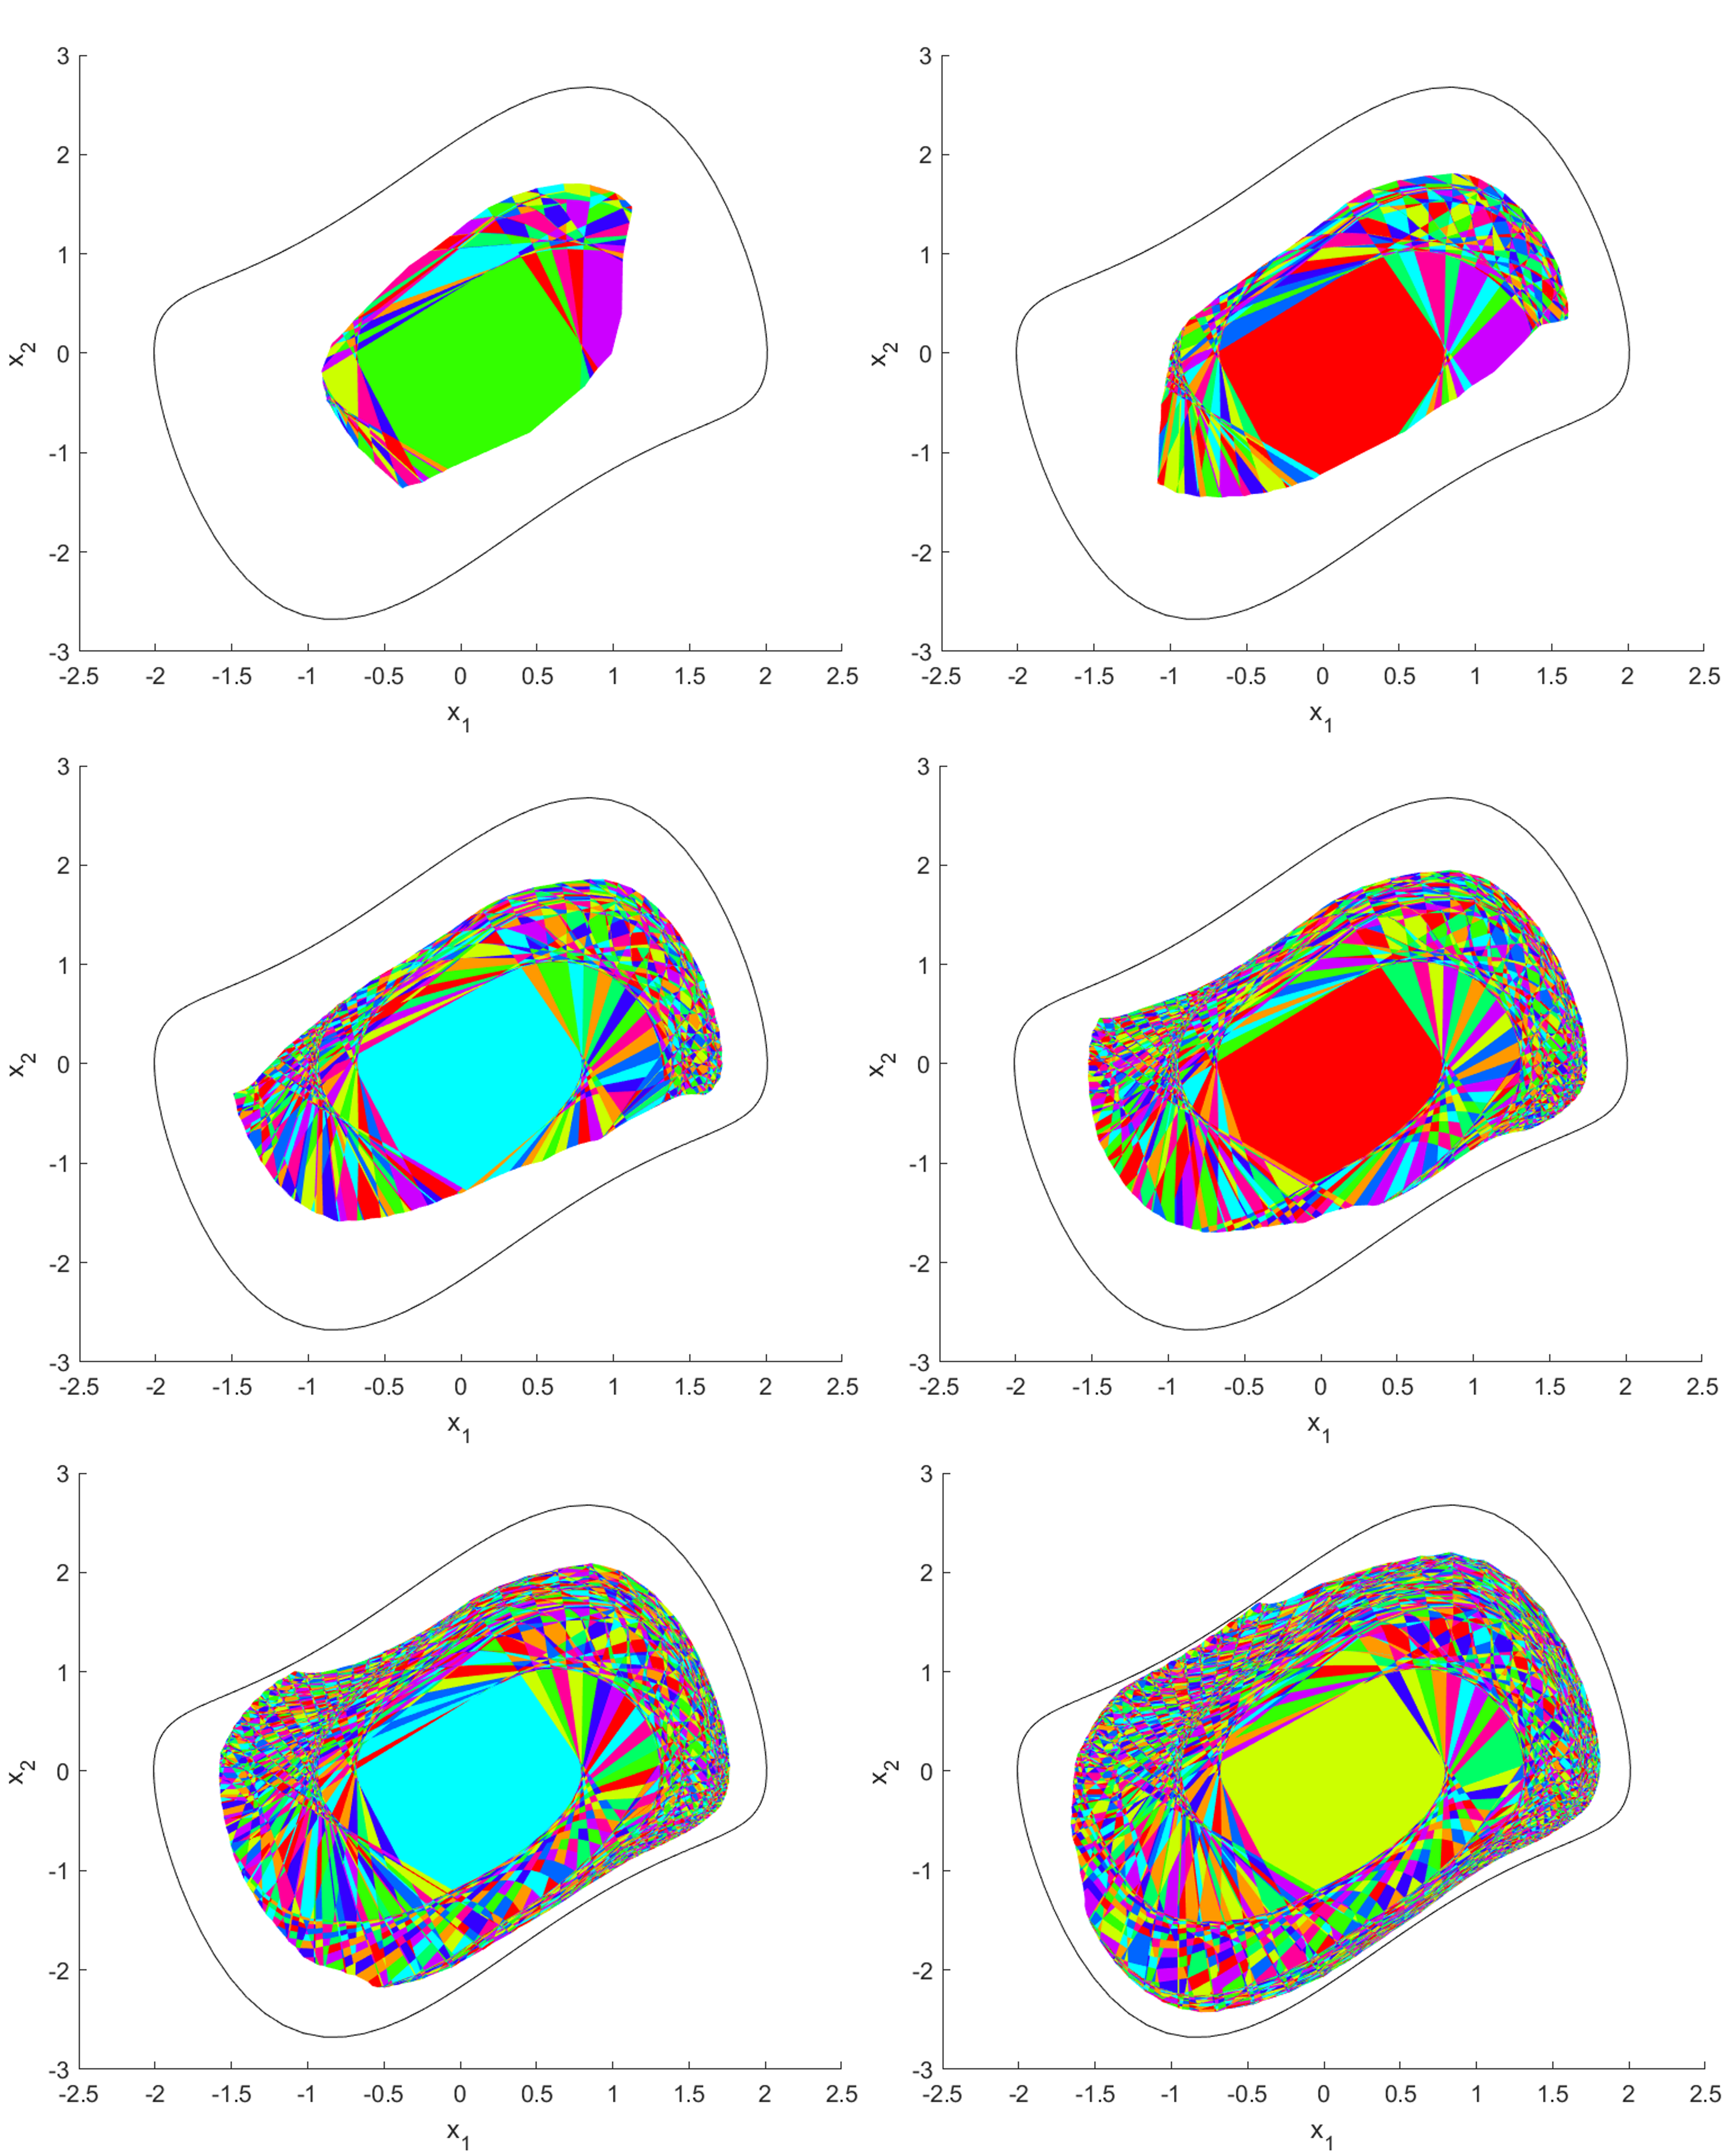
\includegraphics[width=0.98\linewidth]{figs/van_panel_mat.png} 
\setlength\belowcaptionskip{-1.\baselineskip}
\centering
\caption{5, 10, 15, 20, 25, and 30-step regions of attraction (ROAs) for the learned van der Pol system. The learned dynamics network is continuously invertible, implying that preimages of connected sets are connected. This property restricts the space explored with RPM, resulting in a 15x speedup in ROA computation. The black line represents the boundary of the true continuous-time maximal ROA.}
\label{fig:van_panel}
\end{figure}











%%%%%%%%%%%%%%%%%%%%%%%%%%%%%%%%%%%%%%%%%%%%%%%%%%%%%%%%%%%%%%%%%%%%%%%%%%%%%%%%%%%%%
\subsection{Pendulum Example} \label{Pendulum}
In this example we pair our RPM tool with the popular multi-parametric toolbox (MPT3) \cite{MPT3} to find a control invariant set for a learned pendulum model. We first learn a ReLU network that models the continuous-time dynamics
\begin{align}
    \Ddot{\theta} = \frac{u + mgl\sin{\theta}}{ml^2}
\end{align}
as a discrete-time model where $m = 1$kg, $g = 9.81$m/s$^{2}$, $l=1$m, and $\theta$ is measured clockwise from the upright position. 
\textcolor{black}{We repeat the network training and enumeration of affine regions $10$ times and provide ranges for the number of affine regions and computation time in Table \ref{tab:pend_details}.
We run the longer, invariant set computation, on only one of the networks (a network with 217 regions).}

Details of the learned dynamics network are in Table \ref{tab:pend_details}.

% \begingroup
% \setlength{\tabcolsep}{5pt}
% \begin{table}[h]
%     \centering
%     \caption{\textcolor{black}{Pendulum Dynamics Analysis}}
%     {\color{black}\begin{tabular}{c c c}
%         Layer Sizes&\# Affine Regions&Time\\
%         \hline \\ [-1.5ex]
%         $3$, $16$, $16$, $2$ & $217$ & $3$ seconds
%     \end{tabular}}
%     \label{tab:pend_details}
% \end{table} 
% \endgroup

\begingroup
\setlength{\tabcolsep}{5pt}
\begin{table}[h]
    \centering
    \caption{Pendulum Dynamics Analysis}
    {\color{black}\begin{tabular}{c | c}
        Layer Sizes & $3$, $16$, $16$, $2$ \\
        Number of Affine Regions & \textcolor{black}{$217 - 823$} Regions \\
        Time to Enumerate Affine Regions & \textcolor{black}{$2.35 - 4.11$} Seconds
    \end{tabular}}
    \label{tab:pend_details}
\end{table} 
\endgroup




We then use MPT3 to compute the control invariant set shown in Figure \ref{fig:ctrl_inv} with computational details in Table \ref{tab:pend_set}.
% The control invariant set in Figure \ref{fig:ctrl_inv} converged in 61 steps after 5.4 hours of computation, and is represented by 958 polyhedra.

\begingroup
\setlength{\tabcolsep}{5pt}
\begin{table}[h]
    \centering
    \caption{Pendulum Control Invariant Set}
    {\color{black}\begin{tabular}{c c c}
        Algorithm Steps&\# Polyhedra in Set&Time\\
        \hline \\ [-1.5ex]
        $61$ & $958$ & $5.4$ hours
    \end{tabular}}
    \label{tab:pend_set}
\end{table} 
\endgroup

As shown in Figure \ref{fig:ctrl_inv}, the control invariant set is the union of 3 disjoint sets. The leftmost set represents the states for which there is enough control authority to keep the pendulum clockwise of the swing-down position, but not enough to swing back up to upright. The middle set represents the states for which there is enough control authority to keep the pendulum from swinging all the way down. Finally, rightmost set has a similar interpretation to the leftmost set, being the states for which there is enough control authority to keep the pendulum counterclockwise of the swing-down position, but not enough to swing back upright. With the explicit PWA representation given by RPM, the wide array of PWA analysis tools offered by the MPT3 toolbox is able to be leveraged for learned dynamics and controls models.
\begin{figure}[h]
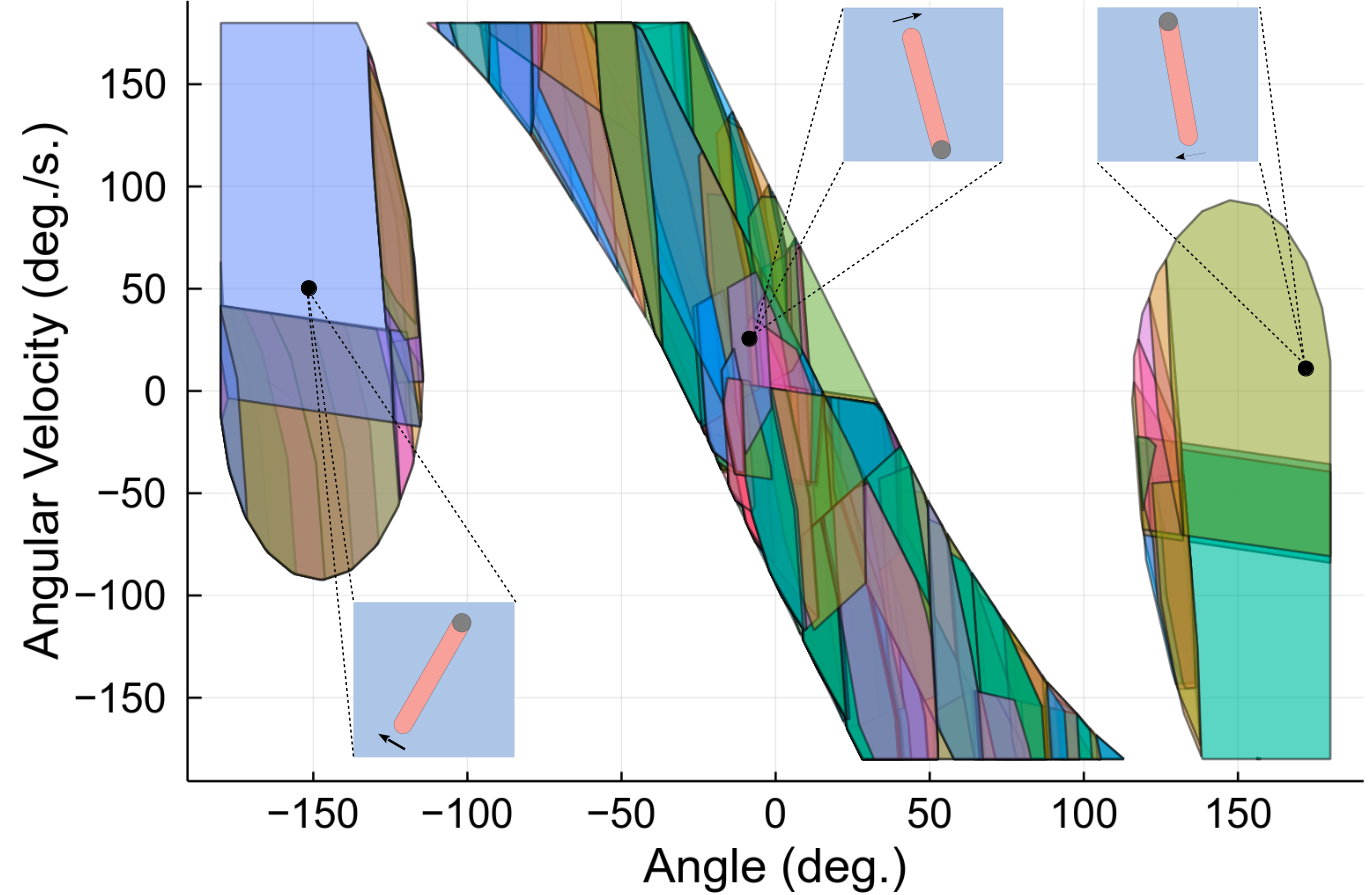
\includegraphics[width=0.85\columnwidth]{figs/ctrl_inv_blowout.png} 
% \setlength\abovecaptionskip{-0.2\baselineskip}
% \setlength\belowcaptionskip{-0.5\baselineskip}
\centering
\caption{A control invariant set for a learned, torque controlled pendulum system. The domain of the dynamics is $\theta \in (-180\degree, 180\degree)$, $\dot{\theta} \in [-180 \degree/\text{s}, 180 \degree/\text{s}]$, $u \in [-5, 5]$ N-m,  where $0\degree$ is upright. Note that we restrict the pendulum so it is not allowed to pass through the down position.  When RPM is paired with MPT3 we are able to compute complicated control invariant sets of learned systems, like this unconnected set, as opposed to convex approximations. Within each connected component a sample state is illustrated to help visualize the possible pendulum configurations.}
\label{fig:ctrl_inv}
\end{figure}

% \begin{figure}
%      \centering
%      \begin{subfigure}[b]{\columnwidth}
%          \centering
%          \includegraphics[width=\textwidth]{figs/ctrl_inv.png}
%          \caption{Control invariant set.}
%          \label{fig:ctrl_inv}
%      \end{subfigure}
%      \hfill
     
%      \begin{subfigure}[b]{0.48\columnwidth}
%          \centering
%          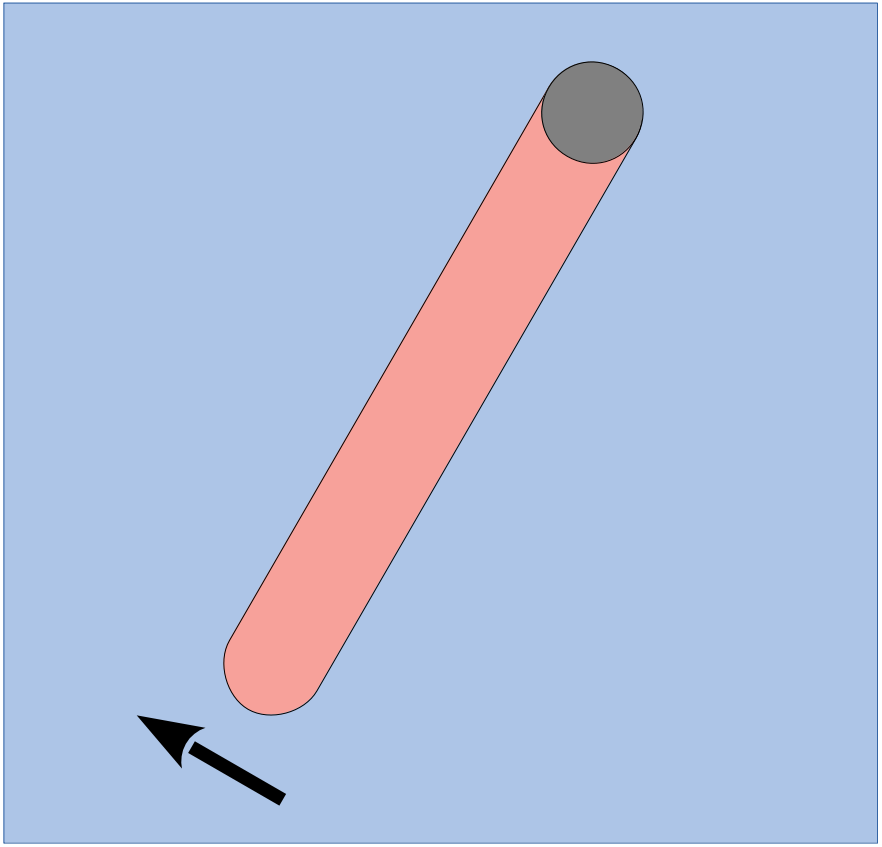
\includegraphics[width=\textwidth]{figs/pend_1.png}
%          \caption{$\theta = -150\degree$, $\dot{\theta} = 50 \degree /$s.}
%          \label{fig:pend_1}
%      \end{subfigure}
%      \hfill
%      \begin{subfigure}[b]{0.48\columnwidth}
%          \centering
%          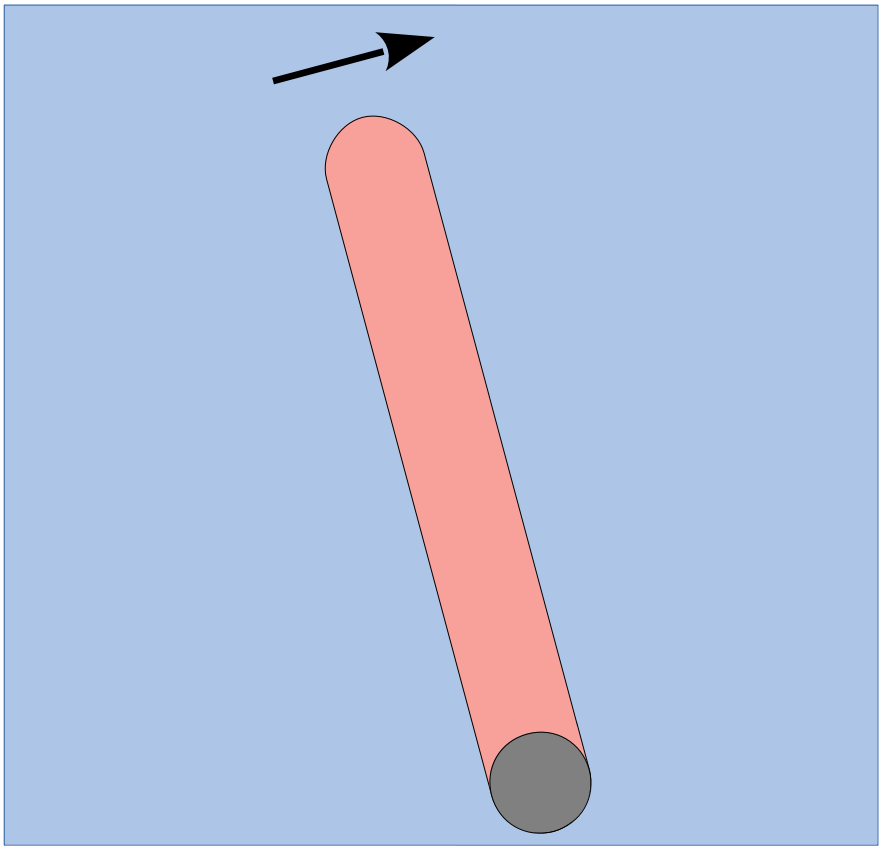
\includegraphics[width=\textwidth]{figs/pend_2.png}
%          \caption{$\theta = -15\degree$, $\dot{\theta} = 25 \degree /$s.}
%          \label{fig:pend_2}
%      \end{subfigure}
%      \hfill
%      \begin{subfigure}[b]{0.48\columnwidth}
%          \centering
%          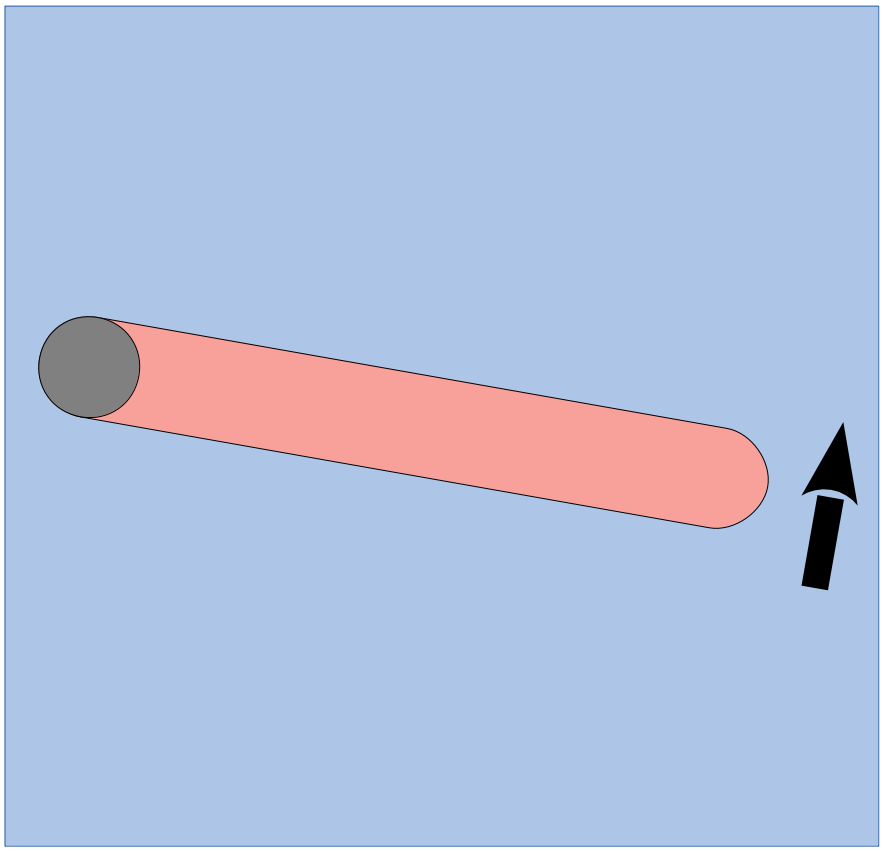
\includegraphics[width=\textwidth]{figs/pend_3.png}
%          \caption{$\theta = 100\degree$, $\dot{\theta} = -170 \degree /$s.}
%          \label{fig:pend_3}
%      \end{subfigure}
%      \hfill
%      \begin{subfigure}[b]{0.48\columnwidth}
%          \centering
%          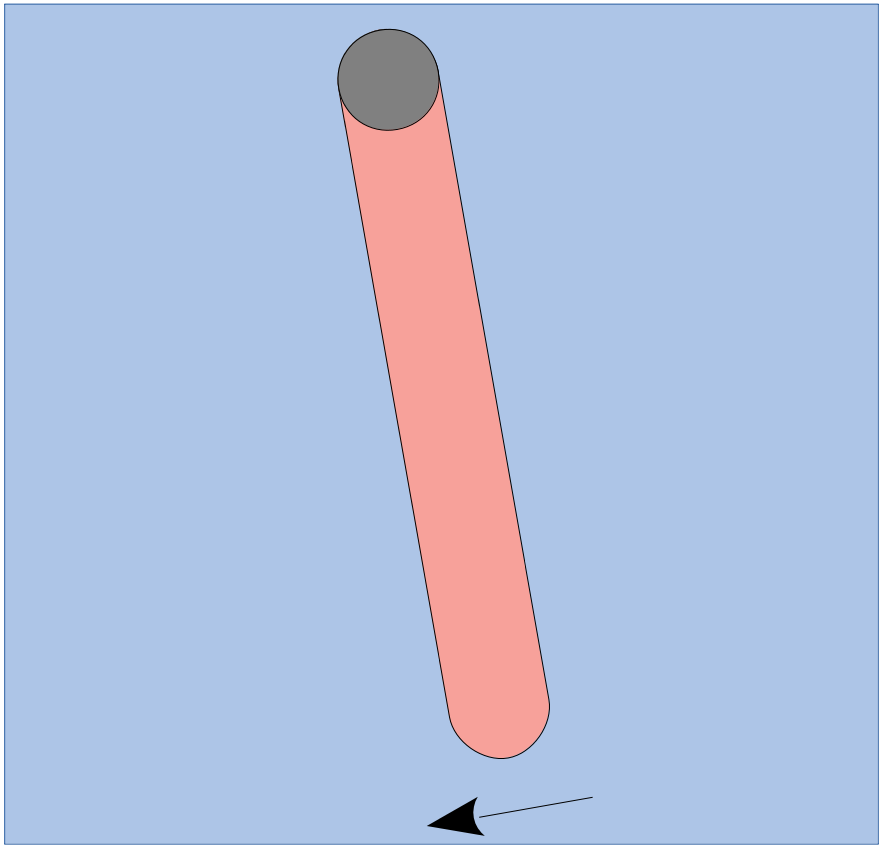
\includegraphics[width=\textwidth]{figs/pend_4.png}
%          \caption{$\theta = 170\degree$, $\dot{\theta} = 10 \degree /$s.}
%          \label{fig:pend_4}
%      \end{subfigure}
%         \caption{A control invariant set (Figure \ref{fig:ctrl_inv}) for a learned, torque controlled pendulum system.  Control invariant set for learned pendulum system with domain $\theta \in [-180\degree, 180\degree]$, $\dot{\theta} \in [-180 \degree/\text{s}, 180 \degree/\text{s}]$, $u \in [-5, 5]$ N-m,  where $0\degree$ is upright.}
%         \label{fig:control_invariant_panel}
% \end{figure}









%%%%%%%%%%%%%%%%%%%%%%%%%%%%%%%%%%%%%%%%%%%%%%%%%%%%%%%
\subsection{Verifying Image-Based Control} \label{Taxinet}
\begin{figure}
    \setlength\abovecaptionskip{1.2\baselineskip}
    \setlength\belowcaptionskip{-0.8\baselineskip}
     \centering
     \begin{subfigure}[b]{0.48\columnwidth}
         \centering
         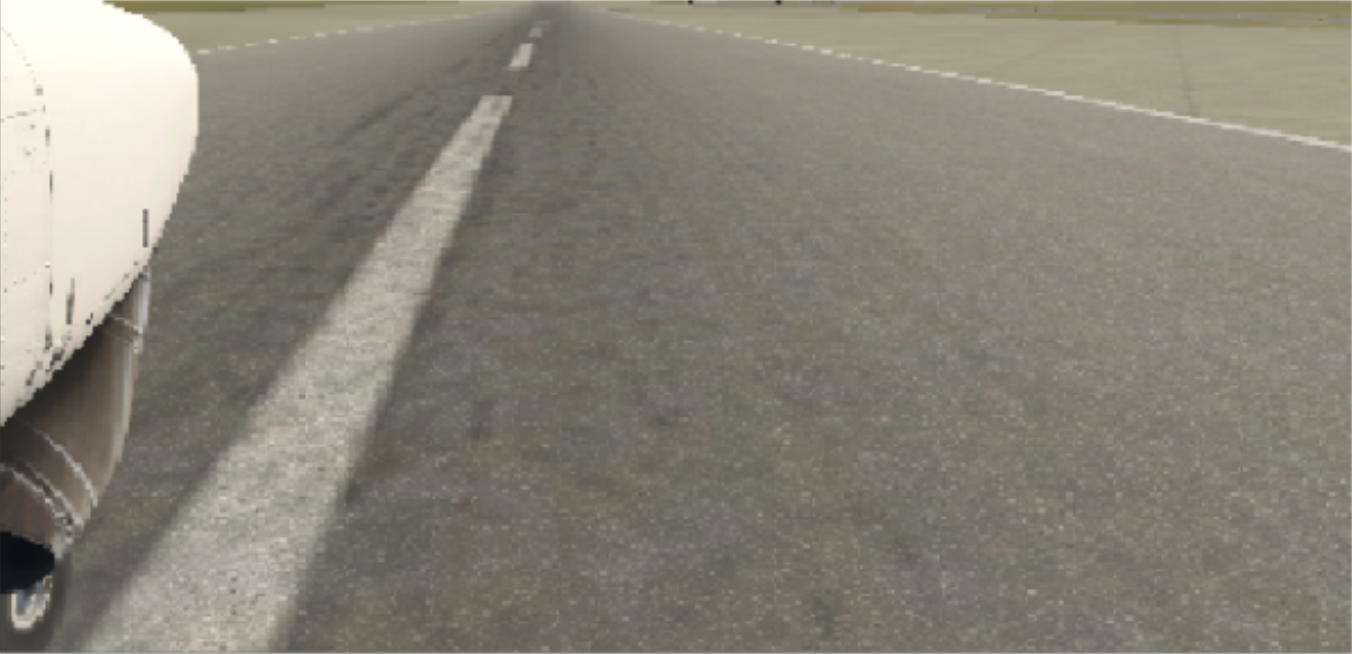
\includegraphics[width=\textwidth]{figs/taxinet_full.png}
         \caption{Full observation.}
         \label{fig:taxinet_full}
     \end{subfigure}
     \hfill
     \begin{subfigure}[b]{0.48\columnwidth}
         \centering
         
\includegraphics[width=\textwidth]{figs/taxinet_coarse.png}
         \caption{Downsampled observation.}
         \label{fig:taxinet_coarse.}
     \end{subfigure}
        \caption{The X-Plane 11 flight simulator is used to generate realistic image observations (left) that are then downsampled (right). The downsampled images are used to learn an image-based controller, as well as to learn an observation model from state to image observation. Putting these two components together along with a learned dynamics network results in closed-loop system dynamics represented as a single ReLU network. These images and learned controller/observation models are from \cite{verify_gan}.}
        \label{fig:taxinet_obs}
\end{figure}

lIn this example we apply the tools of Section \ref{Sec:ROA} to a larger dynamical system that models the closed-loop behavior of a taxiing airplane controlled from camera images.
Our goal is to investigate the set of states that are stabilized by a learned image-based controller by modeling the closed-loop dynamical system with a single ReLU network, and applying the accelerated procedure from Section \ref{Sec:ROA}. 

The specific system we consider was introduced in \cite{verify_gan} where a taxiing airplane is regulated to the centerline of a runway via rudder-angle control input based on images from an onboard camera. Because of the image observation, we cannot model the observation from physical principles. Instead, we modify the learned models in \cite{verify_gan} to obtain a network that approximates the observed image given a state
\begin{align}
    \mathbf{o}_t = F_{obs}(\bx_t),
\end{align}
and a control network that produces a rudder angle command given an observed image
\begin{align}
    u = F_{ctrl}(\mathbf{o}_t).
\end{align}
The continuous time dynamics are
\begin{subequations}
\begin{align}
    \dot{p} &= v\sin{\theta} \\
    \dot{\theta} &= \frac{v}{L}\tan{u}
\end{align}
\end{subequations}
for crosstrack position $p$, heading error $\theta$, rudder angle $u$, and speed $v=5$ m/s. We learn a 1Hz discrete-time model,
\begin{align}
    \bx_{t+1} = F_{dyn}(\bx_t, u),
\end{align}
and then have the closed-loop system
\begin{align}
    \bx_{t+1} = F_{cl}(\bx_t) = F_{dyn}(\bx_t, F_{ctrl} \circ F_{obs}(\bx_t))
\end{align}
which can be represented as one ReLU network.

Next, we use Algorithm \ref{Algo:cell_enumeration} to retrieve the explicit PWA function for $F_{cl}$ over the domain $p \in [-5, 5]$ m., $\theta \in [-15^\circ, 15^\circ]$. 
The resulting PWA function has 244,920 regions, took 3 hours to compute, and was not found to be a homeomorphism.
Timing for these steps is summarized in Table \ref{tab:taxinet_details}.
Although the function is not homeomorphic, when applying the accelerated algorithm from Section \ref{sec:homeo}, we are still guaranteed that all states within this set asymptotically converge to the stable fixed point.


% \begingroup
% \setlength{\tabcolsep}{5pt}
% \begin{table}[h]
%     \centering
%     \caption{\textcolor{black}{Image-Based Control Dynamics Analysis}}
%     {\color{black}\begin{tabular}{c c c}
%         Layer Sizes&\# Affine Regions&Time\\
%         \hline \\ [-1.5ex]
%         $2$, $260$, $260$, $260$, $260$, $20$, $12$, $12$, $16$, $2$ & $244,920$ & $3$ hours
%     \end{tabular}}
%     \label{tab:taxinet_details}
% \end{table} 
% \endgroup

\begingroup
\setlength{\tabcolsep}{5pt}
\begin{table}[h]
    \centering
    \caption{Image-Based Control Dynamics Analysis}
    {\color{black}\begin{tabular}{c | c}
        Layer Sizes & \begin{tabular}{@{}c@{}}$2$, $260$, $260$, $260$, $260$, \\ $20$, $12$, $12$, $16$, $2$\end{tabular} 
          \\
        Number of Affine Regions & $244,920$ Regions \\
        Time to Enumerate Affine Regions & $3$ Hours \\
        Time to Check if Homeomorphism & $0.04$ Seconds \\
        Time to Find Fixed Point & $2$ Seconds \\
        Time to Find Seed ROA & $3$ Seconds
    \end{tabular}}
    \label{tab:taxinet_details}
\end{table} 
\endgroup

This PWA function is significantly larger than other PWA dynamics that have been studied in the literature ($\sim 250,000$ regions vs $\sim 1,000$ regions). 
After computing the explicit PWA function, we find a stable fixed point. Next, we find a seed ROA for each stable fixed point and perform backward reachability to grow the ROAs. During the backward reachability computation, we use a few strategies to make the problem more tractable. First, we restrict the backward reachability algorithm to only explore connected backward reachable sets as described in Section \ref{sec:homeo}. 
Second, to avoid numerical concerns accompanied with very small polyhedra, we compute backward reachable sets iteratively with the 1-step PWA dynamics directly instead of in one shot using concatenated ReLU networks. 
Third, at each step we merge the polyhedra into a union of overlapping polyhedra to reduce the complexity of the set representation.

In Figure \ref{fig:taxi_roa} we show the set of states that our algorithm was able to show is asymptotically stabilized by the learned controller.
This set was computed using $11$ backward reachable steps (11 seconds of trajectory evolution), and is represented as a union of $28,715$ polyhedra.


\begingroup
\setlength{\tabcolsep}{5pt}
\begin{table}[h]
    \centering
    \caption{Image-Based Control ROA}
    {\color{black}\begin{tabular}{c c c}
        Algorithm Steps&\# Polyhedra in Set&Time\\
        \hline \\ [-1.5ex]
        $11$ & $28,715$ & $14$ hours
    \end{tabular}}
    \label{tab:taxinet_roa}
\end{table} 
\endgroup

\begin{figure}
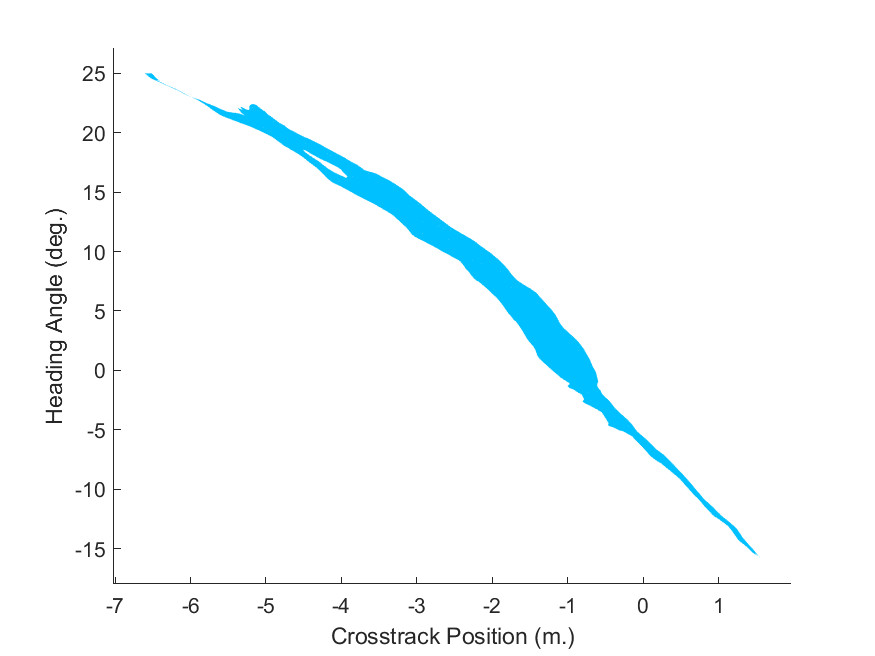
\includegraphics[width = 0.85\linewidth]{figs/taxinet_11.png} 
% \setlength\abovecaptionskip{-0.1\baselineskip}
\setlength\belowcaptionskip{-1.\baselineskip}
\centering
\caption{Set of states that our approach finds are stabilized by the learned controller for the image-based airplane runway taxiing system from Fig.~\ref{fig:taxinet_obs}.
This set is the 11-step backward reachable set for the seed ROA found around the stable fixed point.
This set of states is represented by 28,715 polyhedra.
}
\label{fig:taxi_roa}
\end{figure}

%%%%%%%%%%%%%%%%%%%%%%
\section{Conclusions}
%%%%%%%%%%%%%%%%%%%%%
\label{Sec:Conclusions}
We proposed the Reachable Polyhedral Marching (RPM) algorithm to incrementally construct an exact PWA representation of a ReLU network. 
RPM computes an explicit PWA function representation for a given ReLU network that can then be used to quickly find forward and backward reachable sets of ReLU networks. 
In addition, we demonstrated how, for dynamical systems modeled as ReLU networks, RPM can be leveraged to (i) compute intricate control invariant sets and (ii) certify stability and compute ROAs. 
RPM enumerates affine regions and reachable sets in an incremental and connected fashion, which we show can lead to massive acceleration when computing ROAs.
Lastly, RPM also provides a novel way to determine invertibility of ReLU networks.

In future work we are interested in investigating the homeomorphic properties of ReLU networks. 
There are many studies on the invertibility of neural networks that propose to restrict the network architecture and training such that invertibility is guaranteed with high probability. 
However, these restrictions might be loosened by further understanding the connection between PWA homeomorphisms and ReLU networks. Another area for future work is to use the insights gained from Theorem \ref{thm: activation_flipping} to develop an inverse RPM method for encoding explicit PWA functions as ReLU networks. 
Existing work in this direction yields ReLU networks with many more parameters than necessary, not taking full advantage of the dependency of PWA parameters. Also of interest is the potential to use the PWA decomposition given by RPM to assess where in the domain the ReLU network is likely to generalize well and where it is not.




% Another area for future work is to use RPM for global optimization of ReLU network objective functions. Minimization of an objective function represented as a ReLU network results in a nonconvex optimization problem. However, by extracting the explicit PWA function with RPM, the nonconvex optimization can be solved to global optimality via an LP in reach of the affine regions.


\section*{Acknowledgements}
The authors would like to thank Yue Meng for helpful insights and feedback on the RPM algorithm.

% \addtolength{\textheight}{-12cm}   % This command serves to balance the column lengths
                                  % on the last page of the document manually. It shortens
                                  % the textheight of the last page by a suitable amount.
                                  % This command does not take effect until the next page
                                  % so it should come on the page before the last. Make
                                  % sure that you do not shorten the textheight too much.

%%%%%%%%%%%%%%%%%%%%%%%%%%%%%%%%%%%%%%%%%%%%%%%%%%%%%%%%%%%%%%%%%%%%%%%%%%%%%%%%

%%%%%%%%%%%%%%%%%%%%%%%%%%%%%%%%%%%%%%%%%%%%%%%%%%%%%%%%%%%%%%%%%%%%%%%%%%%%%%%%
%\section*{Appendix}
%Appendixes should appear before the acknowledgment.

%\section*{Acknowledgement}
%To-do.


% \newpage
\bibliographystyle{./IEEEtran} % use IEEEtran.bst style
\bibliography{./IEEEabrv,./IEEEexample}

%%%%%%%%%%%
% \newpage
\appendix 
%%%%%%%%%%%
\label{Sec:Appendix}
%%%%%%%%%%%%%%%%%%%%%%%%%%%%%%%%%%%%%%%%%%%%%%%%%%
%%%%%%%%%%%%%%%%%%%%%%%%%%%%%%%%%%%%%%%%%%%%%%%%%%
% \subsection{Neural Network Verification} \label{ACAS}
% \textcolor{black}{
% Although this paper is focused on analyzing closed-loop control theoretic properties of neural networks, we note that the RPM algorithm can also be used to solve neural network verification problems.
% These problems are typically posed as verifying whether there exists an input that maps to some undesirable set of outputs.
% A common benchmark for neural network verification is a set of 45 distinct policy networks designed to issue advisory warnings to avoid mid-air collisions for unmanned aircraft. Each network has five inputs, \textcolor{black}{six hidden layers with 50 neurons each,} and five outputs (advisories). Inputs are relative distance, angles, and speeds (see \cite{acas} for more details). }

% The appendix of \cite{reluplex} lists ten safety properties the networks should satisfy. Here we consider Property 3. 
% This property is satisfied if the network never outputs a ``Clear of Conflict" advisory when the intruder is directly ahead and moving towards the ownship. 
% We use the backward reachability algorithm to verify whether Property 3 is satisfied. 
% A nonempty backward reachable set implies that some allowable inputs will map to unsafe outputs and the safety property is not satisfied. 
% \textcolor{black}{
% Table \ref{table:verification} shows the results of verifying Property 3 for each of the 45 policy networks. 
% A comparison is given against other exact reachability methods \cite{yang2020reachability,nnenum}, as well as an exact SMT-based method \cite{marabou}.}
% Each algorithm was run on a single core. 
% % We note that a parallelized algorithm is also provided for the face lattice approach \cite{yang2020reachability}, and our RPM algorithm is also amenable to a parallelized implementation. 

% \textcolor{black}{
% The results in Table \ref{table:verification} show that the Marabou algorithm tends to outperform the reachability-based approaches.
% This may be due to the reachability-based approaches returning more information (i.e. reachable sets) than Marabou's SMT approach which returns only whether the safety property is satisfied or not.
% Similarly, we hypothesize that the RPM algorithm tends to be slower than the other reachability algorithms because it outputs not only the PWA representation, but also the graph that defines neighboring affine regions.
% Table \ref{table:verification} also show the advantage of RPM's incremental enumeration (a feature shared by nnenum) when unsafe inputs exist (as is the case for networks $1,7$, $1,8$, and $1,9$).
% The Face Lattice and Marabou approaches are not incremental and do not admit early termination when unsafe inputs exist.
% The number of affine regions that are in the input set specified by Property 3 for each network is given in the table as well.}

% \textcolor{black}{Although the results in this example show RPM is often outperformed in verification tasks, we emphasize that this does not conflict with our stated contributions in which we develop the algorithm to enumerate all affine regions in a connected walk, show how such an algorithm can be used to compute invariant sets, and show how the connected walk can be leveraged to accelerate this computation.}


% % our proposed method when verifying network properties that are found to not hold. Our RPM algorithm is anytime, in the sense that once an unsafe input polyhedron is found, the algorithm can terminate without completing the full reachability computation. This is in contrast to all existing exact reachability methods that proceed layer-by-layer through the network.  They must solve the entire backward reachability problem to conclude any verification result, whether safe or unsafe.

% \begingroup
% \setlength{\tabcolsep}{5pt}
% \begin{table}
% \centering
% \caption{Property 3 Verification Times (s.)}
%  \begin{tabular}{c c c c c c} 
%  Network & Affine Regions & RPM & Face Lattice & nnenum & Marabou \\ [0.5ex] 
%  \hline \\ [-1.5ex]
%  $N_{1,1}$ & 70,631 & 968.42 & 396.14 & \textbf{55.80} & 355.13 \\ 

%  $N_{1,2}$ & 39,529 & 509.00 & 201.53 & \textbf{31.60} & 33.63 \\ 
 
%  $N_{1,3}$ & 12,274 & 168.31 & 60.04 & \textbf{10.40} & 97.14 \\ 

%  $N_{1,4}$ & 4,275 & 51.48 & 22.04 & 4.20 & \textbf{0.30} \\ 

%  $N_{1,5}$ & 4,744 & 54.06 & 25.49 & 4.70 & \textbf{0.68} \\ 

%  $N_{1,6}$ & 1,266 & 15.32 & 7.46 & 1.90 & \textbf{0.07} \\ 

%  $N_{1,7}$ & 500 & \textbf{0.01} & 3.07 & 1.00 & 0.14 \\ 

%  $N_{1,8}$ & 393 & \textbf{0.01} & 2.59 & 0.90 & 0.15 \\ 

%  $N_{1,9}$ & 290 & \textbf{0.01} & 1.93 & 1.00 & 0.15 \\ 

%  $N_{2,1}$ & 16,179 & 200.89 & 72.62 & 12.90 & \textbf{6.47} \\ 

%  $N_{2,2}$ & 6,861 & 85.63 & 33.14 & \textbf{5.90} & 14.83 \\ 
 
%  $N_{2,3}$ & 10,614 & 131.18 & 46.82 & 8.50 & \textbf{3.47} \\ 

%  $N_{2,4}$ & 345 & 3.78 & 2.27 & 1.20 & \textbf{0.06} \\ 

%  $N_{2,5}$ & 2,456 & 30.79 & 11.76 & 2.80 & \textbf{0.22} \\ 

%  $N_{2,6}$ & 253 & 2.57 & 2.01 & 1.10 & \textbf{0.06} \\ 

%  $N_{2,7}$ & 1,199 & 13.37 & 6.24 & 1.80 & \textbf{0.06} \\ 

%  $N_{2,8}$ & 326 & 3.41 & 2.33 & 1.20 & \textbf{0.13} \\ 

%  $N_{2,9}$ & 188 & 2.01 & 1.56 & 1.10 & \textbf{0.06} \\ 

%  $N_{3,1}$ & 5,967 & 70.79 & 29.05 & 5.20 & \textbf{0.34} \\ 

%  $N_{3,2}$ & 36,967 & 471.75 & 206.33 & 29.10 & \textbf{12.38} \\ 
 
%  $N_{3,3}$ & 7,848 & 93.11 & 39.94 & 7.10 & \textbf{0.81} \\ 

%  $N_{3,4}$ & 2,077 & 24.63 & 10.42 & 2.40 & \textbf{0.27} \\ 

%  $N_{3,5}$ & 1,034 & 12.19 & 5.76 & 1.80 & \textbf{0.17} \\ 

%  $N_{3,6}$ & 1,857 & 22.58 & 10.32 & 2.40 & \textbf{0.25} \\ 

%  $N_{3,7}$ & 107 & 1.18 & 1.11 & 1.00 & \textbf{0.06} \\ 

%  $N_{3,8}$ & 654 & 8.31 & 3.94 & 1.50 & \textbf{0.27} \\ 

%  $N_{3,9}$ & 1,201 & 13.58 & 6.16 & 1.90 & \textbf{0.25} \\ 

%  $N_{4,1}$ & 2,276 & 26.33 & 10.44 & \textbf{2.50} & 10.52 \\ 

%  $N_{4,2}$ & 17,894 & 233.65 & 87.89 & \textbf{14.40} & 30.20 \\ 
 
%  $N_{4,3}$ & 20,746 & 270.22 & 113.29 & ERROR & \textbf{9.82} \\ 

%  $N_{4,4}$ & 560 & 6.77 & 3.61 & 1.30 & \textbf{0.14} \\ 

%  $N_{4,5}$ & 351 & 3.80 & 2.04 & 1.20 & \textbf{0.06} \\ 

%  $N_{4,6}$ & 2,496 & 29.58 & 13.18 & 2.90 & \textbf{0.30} \\ 

%  $N_{4,7}$ & 944 & 9.92 & 5.33 & 1.70 & \textbf{0.33} \\ 

%  $N_{4,8}$ & 576 & 6.67 & 3.66 & 1.40 & \textbf{0.06} \\ 

%  $N_{4,9}$ & 611 & 6.93 & 3.96 & 1.50 & \textbf{0.29} \\ 

%  $N_{5,1}$ & 9,461 & 116.76 & 44.02 & \textbf{8.10} & 26.38 \\ 

%  $N_{5,2}$ & 2,104 & 24.25 & 9.19 & 2.50 & \textbf{0.98} \\ 
 
%  $N_{5,3}$ & 2,874 & 33.93 & 15.53 & 3.00 & \textbf{0.38} \\ 

%  $N_{5,4}$ & 758 & 8.77 & 4.29 & 1.60 & \textbf{0.17} \\ 

%  $N_{5,5}$ & 1,305 & 15.32 & 6.49 & 1.80 & \textbf{0.22} \\ 

%  $N_{5,6}$ & 1,143 & 12.64 & 6.71 & 1.90 & \textbf{0.24} \\ 

%  $N_{5,7}$ & 88 & 0.96 & 1.09 & 1.00 & \textbf{0.06} \\ 

%  $N_{5,8}$ & 2,368 & 0.86 & 12.08 & 2.70 & \textbf{0.24} \\ 

%  $N_{5,9}$ & 107 & 1.11 & 1.04 & 1.00 & \textbf{0.06} \\ 

% \end{tabular}
% \label{table:verification}
% \end{table}
% \endgroup











\subsection{Proofs}
In this section we provide a proof for Theorem \ref{thm: activation_flipping}. 
Similar arguments are used to characterize the change in Jacobians of PWA components in \cite{pwa_comp} and the references therein.
\textcolor{black}{We begin with a proof for the first claim of Theorem \ref{thm: activation_flipping} with Lemma \ref{lemma:stationary}.
We then prove the second claim of Theorem \ref{thm: activation_flipping} with Lemma \ref{lemma:flips}, with additional support from Lemma \ref{lemma:affine}.}

% The general framework for finding the activation pattern associated with $P_{k'}$ is to apply the neuron activation flipping rules layer by layer. Flipping a neuron activation in an early layer may alter neuron hyperplane equations in later layers, which in turn may lead to activation flipping in later layers and so on. Each hidden layer neuron is associated with a hyperplane $\ba_{ij}^\top \bx = b_{ij}$ where $i$ denotes the layer and $j$ denotes the neuron index within its layer. Each of these hyperlanes is used to define a halfspace constraint given the neuron activation. We show that the activation of a Type 3 neuron does not change from $P_k$ to $P_{k'}$. We also show that there are only a few ways the hyperplane equation of a Type 1 or 2 neuron can change from $P_k$ to $P_{k'}$. For each of these cases we can determine the proper sense of the associated halfspace constraint for $P_{k'}$ and thus determine the neuron activation in $P_{k'}$. 

% \begin{lemma}[Neuron Types are Complete]
% Each neuron in a hidden layer belongs to one and only one of the Type categories.
% \end{lemma}
% \begin{proof}
% Presented without proof.
% \end{proof}

% \item If $[\ba_{k,ij}^\top\quad  -b_{k,ij}] = \alpha[\ba_\eta^\top\quad -b_\eta]$ for some $\alpha \in \{0,1\}$, then $[\ba_{k',ij}^\top\quad  -b_{k',ij}] = \alpha[\ba_\eta^\top\quad -b_\eta]$ for some $\alpha \in \{-1,0\}$, and the activation $\lambda_{k',ij}$ should be set to ensure this holds.
\subsubsection{Proving Claim 1 of Theorem \ref{thm: activation_flipping}}
\begin{lemma}[Stationary Neurons] \label{lemma:stationary}
If $[\ba_{k,ij}^\top\quad  -b_{k,ij}] \neq \alpha[\ba_\eta^\top\quad -b_\eta]$ for some $\alpha \in \{0,1\}$, then the activation of neuron $ij$ does not change, $\lambda_{k,ij} = \lambda_{k',ij}$.
\end{lemma}
\begin{proof}
\textcolor{black}{We prove this lemma by showing that, under the conditions of the lemma, the constraint induced by the neuron under its activation in $P_k$ remains valid in $P_{k'}$.}

If $[\ba_{k,ij}^\top\quad  -b_{k,ij}] \neq \alpha[\ba_\eta^\top\quad -b_\eta]$ for some $\alpha \in \{0,1\}$, then we know that the constraint $\ba_{k,ij}^\top \bx \le  b_{k,ij}$ is not active on the boundary between $P_k$ and $P_{k'}$. Formally, $\forall \bx \in \interior(P_k \cap P_{k'})$
\begin{align}
    \ba_{k,ij}^{\top}(\bx) \bx < b_{k,ij}(\bx). \label{eq:App_T3}
\end{align}
The inequality must be strict because if the relationship held with equality $\forall \bx \in \interior(P_k \cap P_{k'})$ then we would have $[\ba_{k,ij}^\top\quad  -b_{k,ij}] = \alpha[\ba_\eta^\top\quad -b_\eta]$ for some $\alpha \in \{0,1\}$ (by definition of the neighbor constraint), leading to a contradiction.

Furthermore, if equality held on a strict subset of $\interior(P_k \cap P_{k'})$, then the shared face of $P_k$ and $P_{k'}$ would not be identified by $\ba_\eta^\top \bx = b_\eta$, but instead by both $\ba_\eta^\top \bx = b_\eta$ and  $\ba_{k,ij}^\top \bx = b_{k,ij}$, another contradiction. 

We now know the constraint is not active due to the strict inequality in (\ref{eq:App_T3}).
In addition, note that $\ba_{k,ij}^{\top}(\bx) \bx - b_{k,ij}(\bx)$ is a continuous function of $\bx$. 
From these facts we know $\exists \bm{\delta}$ such that $\bx + \bm{\delta} \in \interior(P_{k'})$ and the inequality remains strict,
\begin{align}
    \ba_{k,ij}^{\top}(\bx + \bm{\delta}) (\bx + \bm{\delta}) < b_{k,ij}(\bx + \bm{\delta}). \label{eq:App_T12}
\end{align}
Therefore, since the constraint associated with such a neuron $ij$ is valid on the interior of both $P_k$ and $P_{k'}$, the neuron activation does not change.

To finish, we note that the case of $\alpha = -1$ is impossible because it would imply that the dimension of $\text{int}(P_k)$ is less than the ambient dimension (contradicting Definition \ref{def:tessellation}).
\end{proof}







\subsubsection{Proving Claim 2 of Theorem \ref{thm: activation_flipping}}
\begin{lemma}[Effects of Activation Flips] \label{lemma:flips}
If \newline $[\ba_{k,ij}^\top\quad  -b_{k,ij}] = \alpha[\ba_\eta^\top\quad -b_\eta]$ for some $\alpha \in \{0,1\}$, then $[\ba_{k',ij}^\top\quad  -b_{k',ij}] = \alpha'[\ba_\eta^\top\quad -b_\eta]$ for some $\alpha' \in \{-1,0\}$.
% Neuron $ij$ (Type 1 or 2) defines a normalized constraint $\ba_{ij}^{\top} \bx \le b_{ij}\ \forall \bx \in P$ where $\ba_{ij} = \alpha\ba_\eta$ for some $\alpha \in \{-1, 0, 1\}$. In addition, $\ba_{ij} = \alpha\ba_\eta \ \forall \bx \in P_{k'}$ for some $\alpha \in \{-1, 0, 1\}$.
\end{lemma}
\begin{proof}
\textcolor{black}{We prove this lemma by first showing that a weaker condition (dependent on $\bx$) holds for all points on the boundary between the regions.
Then, by analyzing this weaker condition for $n$ carefully chosen points on the boundary, we show that the dependence on $\bx$ can be removed and we arrive at the desired result.}

Consider the affine functions defined by neuron $ij$ in regions $P_k$ and $P_{k'}$,
\begin{subequations}
\begin{align}
    \Bar{\ba}_{k,ij}^\top \bx -\Bar{b}_{k,ij} \quad &\forall \bx \in P_k \\
    \Bar{\ba}_{k',ij}^\top \bx -\Bar{b}_{k',ij} \quad &\forall \bx \in P_{k'}
\end{align}
\end{subequations}
(note that the overbar accent indicates the parameters are unnormalized as in (\ref{Eq:HalfspaceDef}). Since ReLU networks are continuous functions, $\forall \bx \in P_k \cap P_{k'}$ we know
\begin{subequations}
\begin{align}
    \Bar{\ba}_{k,ij}^\top \bx -\Bar{b}_{k,ij} &= \Bar{\ba}_{k',ij}^\top \bx -\Bar{b}_{k',ij} \\
    \implies \begin{bmatrix} \multicolumn{2}{c}{\Bar{\ba}_{k',ij}^\top} & -\Bar{b}_{k',ij} \end{bmatrix} \begin{bmatrix} \bx \\ 1 \end{bmatrix} &= 
    \begin{bmatrix} \multicolumn{2}{c}{\Bar{\ba}_{k,ij}^\top} & -\Bar{b}_{k,ij} \end{bmatrix} \begin{bmatrix} \bx \\ 1 \end{bmatrix} \\
    \implies \begin{bmatrix} \multicolumn{2}{c}{\Bar{\ba}_{k',ij}^\top} & -\Bar{b}_{k',ij} \end{bmatrix} \begin{bmatrix} \bx \\ 1 \end{bmatrix} &= 
    \beta \begin{bmatrix}  \multicolumn{2}{c}{\ba_{\eta}^\top} & -b_{\eta} \end{bmatrix} \begin{bmatrix} \bx \\ 1 \end{bmatrix}
\end{align}
\end{subequations}
for some $\beta \ge 0$. Thus, we know the normalized constraint $\ba_{k',ij}^\top \bx \le b_{k',ij}$ must satisfy
\begin{align}
    \begin{bmatrix} \multicolumn{2}{c}{\ba_{k',ij}^\top} & -b_{k',ij} \end{bmatrix}  \begin{bmatrix} \bx \\ 1 \end{bmatrix} &=  
    \alpha' \begin{bmatrix} \ba^\top_\eta & -b_\eta \end{bmatrix} 
    \begin{bmatrix} \bx \\ 1 \end{bmatrix} \label{eq:x_depend}
\end{align}
for some $\alpha' \in \{-1,0,1\}$ and $\forall \bx \in P_k \cap P_{k'}$. We next seek to remove this relationship's dependence on $\bx$.

We know $P_k \cap P_{k'}$ is a subset of the $n-1$-dimensional affine span $\{\bx \mid \ba_\eta^\top \bx = b_\eta \}$. Since $\vert P_k \cap P_{k'} \vert_{n-1} \neq 0$ there exist $\bx_1, \ldots, \bx_{n} \in P_k \cap P_{k'}$ that define the vertex points of an $n-1$-dimensional simplex on $P_k \cap P_{k'}$. The vertices of a simplex are known to be affinely independent. Therefore, by Lemma \ref{lemma:affine}, the vectors
\begin{align}
    \begin{bmatrix} \bx_1 \\ 1 \end{bmatrix}, \ldots, \begin{bmatrix} \bx_{n} \\ 1 \end{bmatrix} \in \mathbb{R}^{n+1}
\end{align}
are linearly independent. Next, consider the matrix formed by these vectors
\begin{align}
    \mathbf{X} = \begin{bmatrix} \bx_1^\top & 1 \\ \vdots & \vdots \\ \bx_{n}^\top & 1 \end{bmatrix} \in \mathbb{R}^{n \times n+1}.
\end{align}
From (\ref{eq:x_depend}), and since $\ba_\eta^\top \bx_i - b_\eta = 0 \quad \forall i \in 1,\ldots,n$,
\begin{subequations}
\begin{align}
    \mathbf{X} \begin{bmatrix} \ba_{k',ij} \\ -b_{k',ij} \end{bmatrix}  &= \alpha' \mathbf{X}  \begin{bmatrix} \ba_\eta \\ -b_\eta \end{bmatrix}\\
    \mathbf{X} \begin{bmatrix} \ba_{k',ij} \\ -b_{k',ij} \end{bmatrix} &= \mathbf{0}.
\end{align}
\end{subequations}

By the rank-nullity theorem, nullity$(\mathbf{X}) = 1$ (rank is $n$ by construction and $\mathbf{X} \in \mathbb{R}^{n \times n+1}$). Furthermore, since both $[\ba_{k',ij}^\top \quad -b_{k',ij}]^\top$ and $[\ba_\eta^\top \quad -b_\eta]^\top$ lie in a single-dimensional nullspace, they must be scalar multiples of each other.
Thus, for some $\alpha' \in \{-1,0,1\}$,
\begin{subequations}
    \begin{align}
    [\ba_{k',ij}^\top \quad -b_{k',ij}]^\top, [\ba_\eta^\top \quad -b_\eta]^\top \in \text{null}(\mathbf{X}) \\
    \implies [\ba_{k',ij}^\top\quad  -b_{k',ij}] = \alpha'[\ba_\eta^\top\quad -b_\eta].
\end{align}
\end{subequations}

Lastly, $\begin{bmatrix} \multicolumn{2}{c}{\ba_{k',ij}^\top} & -b_{k',ij} \end{bmatrix} = \begin{bmatrix} \ba^\top_\eta & -b_\eta \end{bmatrix}$ cannot hold as it leaves $P_{k'}$ lower than the ambient dimension, so $\alpha' \neq 1$. Thus, we arrive at the desired result.
\end{proof}



\begin{lemma}[Affine Independence to Linear Independence]\label{lemma:affine}
Given affinely independent vectors $\bx_1,\ldots,\bx_k \in \mathbb{R}^n$, $[\bx_1^\top \quad 1 ]^\top, \ldots, [ \bx_k^\top \quad 1 ]^\top \in \mathbb{R}^{n+1}$ are linearly independent.
\end{lemma}
\begin{proof}
The vectors $[\bx_1^\top \quad 1 ]^\top, \ldots, [ \bx_k^\top \quad 1 ]^\top$ are linearly independent if and only if
\begin{subequations}
\begin{align}
    \lambda_1\begin{bmatrix} \bx_1 \\ 1 \end{bmatrix} + \lambda_2\begin{bmatrix} \bx_2 \\ 1 \end{bmatrix} + \ldots + \lambda_k\begin{bmatrix} \bx_{k} \\ 1 \end{bmatrix} &= \mathbf{0} \\
    \implies \lambda_1 = \lambda_2 = \ldots = \lambda_k &= 0.
\end{align}
\end{subequations}
This condition is equivalent to
\begin{subequations}
\begin{align}
    \begin{rcases}
    \lambda_1 \bx_1 + \lambda_2 \bx_2 + \ldots + \lambda_k \bx_k &= \mathbf{0} \\
    \lambda_1 + \lambda_2 + \ldots + \lambda_k &= 0
  \end{rcases} \\
  \implies \lambda_1 = \lambda_2 = \ldots = \lambda_k &= 0,
\end{align}
\end{subequations}
i.e. $\bx_1,\ldots,\bx_k$ are affinely independent.
\end{proof}


% \begin{lemma}[Number of Affinely Independent Vectors]
% Given a linear subspace $S$ of dimension $n-1$ and affine hull $S + \bb$ for some $\bb \notin S$, there exists a set of $n$ affinely independent vectors in $S + \bb$. 
% \end{lemma}
% \begin{proof}
% Suppose the vectors
% \begin{align*}
%     \bx_1, \ldots, \bx_n
% \end{align*}
% are linearly independent.

% Consider the set of affinely independent vectors
% \begin{align*}
%     \bx_1, \ldots, \bx_k \in S + \bb
% \end{align*}
% where 
% \begin{align*}
%     \lambda_1\bx_1 + \ldots + \lambda_k\bx_k = \mathbf{0}.
% \end{align*}
% Then
% \begin{align*}
%     \lambda_1(\bx_1 - \bb) + \ldots + \lambda_k(\bx_k - \bb) = -(\lambda_1 + \ldots + \lambda_k)\bb.
% \end{align*}
% We know $\bx_i - \bb \in S \quad \forall i \in 1,\ldots,k$, but that $\bb \notin S$. So the only way for the above equality to hold is if \begin{align*}
%     \lambda_1 + \ldots + \lambda_k = 0.
% \end{align*}
% Which implies that the set of vectors $\bx_1, \ldots, \bx_k$ is linearly independent in $\mathbb{R}^n$.

% \end{proof}







% In addition, $\forall \bx \in P_k \cap P_{k'}$,
% \begin{align*}
%     \ba_\eta^{\top} \bx - b_\eta &= 0 \\
%     \implies \begin{bmatrix}
%                 \ba^\top_\eta & -b_\eta 
%              \end{bmatrix} \begin{bmatrix} \bx \\ 1 \end{bmatrix} &= 0.
% \end{align*}
% Thus, $\forall \bx \in P_k \cap P_{k'}$,
% \begin{align*}
%     \begin{bmatrix} \multicolumn{2}{c}{\Bar{\ba}_{k,ij}^\top - \Bar{\ba}_{k',ij}^\top} & -\Bar{b}_{k,ij} + \Bar{b}_{k',ij} \end{bmatrix}  \begin{bmatrix} \bx \\ 1 \end{bmatrix} =  
%     \begin{bmatrix} \ba^\top_\eta & -b_\eta \end{bmatrix} 
%     \begin{bmatrix} \bx \\ 1 \end{bmatrix} \\
%     \implies \begin{bmatrix} \multicolumn{2}{c}{\Bar{\ba}_{k',ij}^\top} & -\Bar{b}_{k',ij} \end{bmatrix}  \begin{bmatrix} \bx \\ 1 \end{bmatrix} =  
%     (\begin{bmatrix} \multicolumn{2}{c}{\Bar{\ba}_{k,ij}^\top} & -\Bar{b}_{k,ij} \end{bmatrix} -
%     \begin{bmatrix} \ba^\top_\eta & -b_\eta \end{bmatrix}) 
%     \begin{bmatrix} \bx \\ 1 \end{bmatrix}.
% \end{align*}
% Furthermore, since we assume $[\ba_{k,ij}^\top\quad  -b_{k,ij}] = \alpha[\ba_\eta^\top\quad -b_\eta]$ for some $\alpha \in \{0,1\}$,




% for a Type 1 or 2 neuron $ij$ in any layer $i$, $\Bar{\ba}_{k',ij} \propto \ba_\eta$ (since we already established that $\Bar{\ba}_{k,ij} \propto \ba_\eta$).

% If $[\Bar{\ba}_{k,ij}^\top\quad  -\Bar{b}_{k,ij}] \propto [\ba_\eta^\top\quad -b_\eta]$, then $[\Bar{\ba}_{k',ij}^\top\quad  -\Bar{b}_{k',ij}] \propto [\ba_\eta^\top\quad -b_\eta]$. Now, when we normalize the hyperlanes as in (REF), we have $[\ba_{k,ij}^\top\quad  -b_{k,ij}] = \alpha[\ba_\eta^\top\quad -b_\eta]$ for some $\alpha \in \{-1,0,1\}$, then $[\ba_{k',ij}^\top\quad  -b_{k',ij}] = \alpha[\ba_\eta^\top\quad -b_\eta]$ for some $\alpha \in \{-1,0,1\}$. Furthermore, we know $P_{k'} \subset \ba_{k',ij}^\top \bx \le  b_{k',ij}$, from which we can conclude the direction of the new constraint must be opposite the direction of the neighbor constraint. This leads to the desired result that if $[\ba_{k,ij}^\top\quad  -b_{k,ij}] = \alpha[\ba_\eta^\top\quad -b_\eta]$ for some $\alpha \in \{0,1\}$, then $[\ba_{k',ij}^\top\quad  -b_{k',ij}] = \alpha[\ba_\eta^\top\quad -b_\eta]$ for some $\alpha \in \{-1,0\}$.



%%
% Next, if, for Type 1 and 2 neurons in layer $k$, $\ba_{kj}^{c'} \propto \ba_\eta$ then $\ba_{k+1\ j}^{c'} = \ba_{k+1\ j}^{c} + \beta\ba_\eta$ for some scalar $\beta$ and $\ba_{k+1\ j}^{c'} \propto \ba_\eta$ for Type 1 and 2 neurons in layer $k+1$. To see why this is true, we first note the result from Lemma XX that Type 3 neuron activations do not change from $c$ to $c'$. 

% First, consider a Type 1 neuron in the first hidden layer. To define a valid constraint for $c'$ the activation must clearly be flipped but $[\ba_{1j}\ \  -b_{1j}]$ remains unchanged since it is just the $j$th row of $\tilde{\mathbf{W}}_1$ and there are no previous flipping neurons to affect it. Similarly $[\ba_{1j}\ \ -b_{1j}]$ for a Type 2 neuron remains the same and the activation of such a neuron is always $0$.

% Now consider a Type 1 or 2 neuron in the second hidden layer. We know
% \begin{align}
%     \begin{bmatrix}
%         \ba_{2j} & -b_{2j}
%     \end{bmatrix} =  
%     \tilde{\mathbf{W}}_2[j,:]  diag(AP_{1})\tilde{\mathbf{W}}_1. \\
%     \implies
%     \label{eq:layer2}
% \end{align}
% Clearly the row vector $[\ba_{2j}\ \ -b_{2j}]$ is a linear combination of the rows of $diag(AP_{1})\tilde{\mathbf{W}}_1$. To determine the updated hyperplane equation for this neuron we use $AP_1^{c'}$ in (\ref{eq:layer2}) instead of $AP_1^{c}$. Since the only neurons in the first hidden layer to change activation are Type 1 (scalar multiples of $[\ba_{n}\ \ -b_{n}]$), the effect of this is to add a scalar multiple of $[\ba_{n}\ \ -b_{n}]$ to $[\ba_{2j}\ \ -b_{2j}]$ defined for $\bx \in c$. Thus, for a Type 1 neuron in the second hidden layer, $[\ba_{2j}\ \ -b_{2j}]$ defined for $\bx \in c'$ is also a scalar multiple of the neighbor hyperplane. 

% Similarly, the updated $\ba_{2j}$ of a Type 2 constraint will be a scalar multiple of $\ba_\eta$. But the updated $b_{2j}$ of a Type 2 constraint need not be a scalar multiple of $b_\eta$ since $b_{2j}$ defined for $\forall \bx \in c$ may have been positive. 

% It should be clear now that in deeper layers, the update to any $\ba_{ij}$ will be the addition of a scalar multiple of $\ba_\eta$. And since Type 1 and 2 neurons have $\ba_{ij}$ which are already scalar multiples of $\ba_\eta$, their updated quantities remain scalar multiples of $\ba_\eta$. Which, as stated above, implies $\ba_{ij} = \alpha\ba_\eta$ and $\alpha \in \{-1, 0, 1\}$.



% Given the above lemmas we know that the updated hyperplane equations for Type 1 and 2 neurons satisfy $\ba_{ij} = \alpha\ba_\eta$ for some $\alpha \in \{-1, 0, 1\}$. It also must be the case that either $\tilde{\mathbf{b}}_{ij} \ge \alpha\mathbf{b}_\eta$ or $\tilde{\mathbf{b}}_{ij} < \alpha\mathbf{b}_\eta$. This leaves us with six possible cases for which an updated hyperplane equation could fall into. We now enumerate each case and determine the appropriate halfspace constraint for each, which is used to determine the neuron activation. We first assume the neuron activation from $c$ also holds in $P_{k'}$ and flip the activation if need be. That is, we initially assume $\ba_{ij}^{\top} \bx \le b_{ij}$.

% \begin{lemma}
% If $\ba_{ij} = \mathbf{0}$ and $b_{ij} \ge 0$, the constraint is valid and the neuron activation is unchanged.
% \end{lemma}
% \begin{proof}
% $\mathbf{0}^{\top} \bx \le b_{ij}$ is always satisfied.
% \end{proof}


% \begin{lemma}
% If $\ba_{ij} = \mathbf{0}$ and $b_{ij} < 0$, the constraint is invalid and the neuron activation is changed.
% \end{lemma}
% \begin{proof}
% $\mathbf{0}^{\top} \bx \le b_{ij}$ is never satisfied.
% \end{proof}

% For the following results we recognize that for $\ba_{ij}^{\top} \bx \le b_{ij}$ to be a valid constraint for $c'$, the sets $\{\bx \mid \ba_{ij}^{\top} \bx \le b_{ij} \}$ and $\{\bx \mid \ba_\eta^{\top} \bx \le b_\eta \}$ must intersect in a full dimensional polyhedron that contains the hyperplane $\ba_\eta^{\top} \bx = b_\eta$. Put another way, for $\ba_{ij}^{\top} \bx \le b_{ij}$ to be valid, it must imply that $\ba_\eta^{\top} \bx = b_\eta - s$ holds $\forall s \in [0, u]$ for some $u > 0$. 
% \begin{lemma}
% If $\ba_{ij} = \ba_\eta$ and $b_{ij} \ge b_\eta$, the constraint is valid and the neuron activation is unchanged.
% \end{lemma}
% \begin{proof}
% \begin{align*}
%     \ba_{ij}^{\top} \bx &\le b_{ij} \\
%     \implies \ba_\eta^{\top} \bx &\le b_\eta + \delta \text{ (where }b_{ij} = b_\eta + \delta,\ \delta \ge 0) \\
%     \implies \ba_\eta^{\top} \bx &= b_\eta + \delta - \tilde{s},\ \tilde{s} \ge 0 \\
%     \implies \text{if } s &= \tilde{s} - \delta,\ \text{then }  s \in [0, \infty) \\
%     \implies \ba_\eta^{\top} \bx &= b_\eta - s \text{ holds } \forall s \in [0, \infty)
% \end{align*}
% \end{proof}


% \begin{lemma}
% If $\ba_{ij} = \ba_\eta$ and $b_{ij} < b_\eta$, the constraint is invalid and the neuron activation is changed.
% \end{lemma}
% \begin{proof}
% \begin{align*}
%     \ba_{ij}^{\top} \bx &\le b_{ij} \\
%     \implies \ba_\eta^{\top} \bx &\le b_\eta + \delta \text{ (where }b_{ij} = b_\eta + \delta,\ \delta < 0) \\
%     \implies \ba_\eta^{\top} \bx &= b_\eta + \delta - \tilde{s},\ \tilde{s}\ge 0 \\
%     \implies \text{if } s &= \tilde{s} - \delta,\ \text{then }  s \notin [0, \delta) \\
%     \implies \nexists u\ s.t.\  \ba_\eta^{\top} \bx &= b_\eta - s \text{ holds } \forall s \in [0, u]
% \end{align*}
% \end{proof}


% \begin{lemma}
% If $\ba_{ij} = -\ba_\eta$ and -$b_{ij} < b_\eta$, the constraint is valid and the neuron activation is unchanged.
% \end{lemma}
% \begin{proof}
% \begin{align*}
%     \ba_{ij}^{\top} \bx &\le b_{ij} \\
%     \implies -\ba_\eta^{\top} \bx &\le b_{ij} \\
%     \implies \ba_\eta^{\top} \bx &\ge -b_{ij} \\
%     \implies \ba_\eta^{\top} \bx &\ge b_\eta - \delta \text{ (where }-b_{ij} = b_\eta - \delta,\ \delta > 0) \\
%     \implies \ba_\eta^{\top} \bx &= b_\eta - \delta + \tilde{s},\ \tilde{s}\ge 0 \\
%     \implies \text{if } s &= -\tilde{s} + \delta,\ \text{then }  s \in [0, \delta] \\
%     \implies \ba_\eta^{\top} \bx &= b_\eta - s \text{ holds } \forall s \in [0, \delta]
% \end{align*}
% \end{proof}


% \begin{lemma}
% If $\ba_{ij} = -\ba_\eta$ and -$b_{ij} \ge b_\eta$, the constraint is invalid and the neuron activation is changed.
% \end{lemma}
% \begin{proof}
% \begin{align*}
%     \ba_{ij}^{\top} \bx &\le b_{ij} \\
%     \implies -\ba_\eta^{\top} \bx &\le b_{ij} \\
%     \implies \ba_\eta^{\top} \bx &\ge -b_{ij} \\
%     \implies \ba_\eta^{\top} \bx &\ge b_\eta - \delta \text{ (where }-b_{ij} = b_\eta - \delta,\ \delta \le 0) \\
%     \implies \ba_\eta^{\top} \bx &= b_\eta - \delta + \tilde{s},\ \tilde{s}\ge 0 \\
%     \implies \text{if } s &= -\tilde{s} + \delta,\ \text{then }  s \notin (0, \infty) \\
%     \implies \nexists u\ s.t.\  \ba_\eta^{\top} \bx &= b_\eta - s \text{ holds } \forall s \in [0, u]
% \end{align*}
% \end{proof}


\end{document}